% -------------------------------------------------------------
% Suggested template for the SDU Software Engineering Course, 2025
%
% -------------------------------------------------------------

\documentclass[12pt,                                          % Main text font size
               a4paper,                                       % Paper size
               openany                                 % Chapters start on odd pages (right)
              ]{report}                               % Print two-sided, LaTeX 'report' template

% -------------------------------------------------------------
% PACKAGES - Only load if necessary / used
% -------------------------------------------------------------
\usepackage{microtype}                                        % Tweak font spacing for aesthetics
\usepackage{cmbright}                                         % SS font - Comment this line for LaTeX base font
\usepackage[utf8]{inputenc}                                   % Includes letters with accents
\usepackage[T1]{fontenc}                                      % 8-bit encoding with 256 glyphs
\usepackage[colorlinks=true, allcolors=black]{hyperref}       % Hyper-references in PDF (e.g. urlcolor=blue)
\usepackage{fancyhdr}                                         % Headers and footers
\usepackage{subfigure}                                        % Multiple figures environment
\usepackage{amsmath}                                          % Standard maths
\usepackage{amssymb}                                          % Standard maths symbols
\usepackage{graphicx}                                         % Include graphics
\usepackage{booktabs}                                         % Professional tables
\usepackage[english]{babel}                                   % Babel and language definitions
\usepackage[a4paper,                                          % Paper size
            top = 35mm,                                       % Top margin
            bottom = 30mm,                                    % Bottom margin
            left = 35mm,                                      % Left margin
            right = 25mm]{geometry}                           % Right margin
\usepackage{nomencl}                                          % Include nomenclature
\usepackage[page,toc,titletoc,title]{appendix}                % Include appendixes
\usepackage{csquotes}                                         % For inline and display quotations
\usepackage{lipsum}                                           % Generate automatic text - Lorem Ipsum
\usepackage{moreverb}                                         % Output for word and character count
\usepackage{tcolorbox}                                        % Coloured boxes
\usepackage{xcolor}                                           % Advanced colours
\usepackage{soul}                                             % Highlight text and other text things
\usepackage{caption}                                          % Manage captions in floats
\usepackage{chemfig,chemformula}                              % Use chemistry formulae
\usepackage{pgfgantt}                                         % Use a Gantt chart
\usepackage{pdflscape}                                        % Landscape pages
\usepackage{cite}                                             % Compressed and sorted lists of citations
\usepackage{listings}                                         % Displayed code
\usepackage{siunitx}                                          % Easy unit control
\usepackage{titlesec}
\usepackage{float}
\usepackage{enumitem}
\usepackage{parskip}
\usepackage{pgfplots}
\usepackage{hyperref}
\usepackage{pdfpages}
\usepackage{array}
\usepackage{layout}
\usepackage[acronym]{glossaries}
\pgfplotsset{compat=1.18}
\usepgfplotslibrary{dateplot}

% -------------------------------------------------------------
% USER VARIABLES AND DEFINITIONS                              % EDIT THIS SECTION
% -------------------------------------------------------------
%\newcommand{}{}
\newcommand{\theTitle}{Development of Software Systems (F26)}            % Thesis title
\newcommand{\runningTitle}{2nd Semester Project (F26)}                % Short title for headers
\newcommand{\thegroup}{\textbf{Group 11}}                  % Author name

\newcommand{\subtitle}[1]{%
  \\[0.5em] % adjust vertical space as needed
  {\Large\textit{\textcolor{mygrey}{#1}}}%
}


\definecolor{mygrey}{RGB}{64,64,64}
                      % Define your own colours
\definecolor{ocre}{RGB}{45,105,145} 
\definecolor{barblue}{RGB}{153,204,254}                       % Used in Gantt chart
\definecolor{groupblue}{RGB}{51,102,254}                      % Used in Gantt chart
\definecolor{linkred}{RGB}{165,0,33}                          % Used in Gantt chart

\captionsetup[table]{skip=6pt}                                % Gap between captions and tables
\graphicspath{{Images/}}                                      % Path to folder where pictures are stored
\makenomenclature                                             % Create a nomenclature
\setlength{\nomlabelwidth}{10mm}                              % Set width of nomenclature label
\setlength{\headheight}{14pt}                                 % Minimum hadhight length
% -------------------------------------------------------------
% CREATE ABBREVIATIONS
% -------------------------------------------------------------
\makeglossaries

\newacronym{sdu}{SDU}{University of Southern Denmark}
\newacronym{bsc}{BSc.}{Bachelor of Science}
\newacronym{fr}{FR}{Functional Requirement}
\newacronym{nfr}{NFR}{Non-Functional Requirement}
\newacronym{gui}{GUI}{Graphical User Interface}
\newacronym{am}{AM}{Asset Manager}
\newacronym{sdm}{SDM}{Source Data Manager}
\newacronym{opt}{OPT}{Optimizer}
\newacronym{rdm}{RDM}{Result Data Manager}
\newacronym{dv}{DV}{Data Visualization}
\newacronym{csv}{CSV}{Comma Separated Values}
\newacronym{mvvm}{MVVM}{Model View View-Model}
\newacronym{sm}{SM}{Scrum Master}
\newacronym{dt}{DT}{Development Team}
\newacronym{po}{PO}{Product Owner}
\newacronym{uml}{UML}{Unified Modeling Language}
\newacronym{crc}{CRC}{Class Responsibility Collaboration}
\newacronym{xml}{XML}{Extensible Markup Language}
\newacronym{xlsx}{XLSX}{Microsoft Excel Open \acrshort{xml} Spreadsheet}
\newacronym{ui}{UI}{User Interface}
\newacronym{srp}{SRP}{Single Responsibility Principle}
\newacronym{ocp}{OCP}{Open/Closed Principle}
\newacronym{lsp}{LSP}{Liskov Substitution Principle}
\newacronym{isp}{ISP}{Interface Segregation Principle}
\newacronym{dip}{DIP}{Dependency Injection Principle}
\newacronym{solid}{SOLID}{\acrshort{srp} \acrshort{ocp} \acrshort{lsp} \acrshort{isp} \acrshort{dip}}
\newacronym{xaml}{XAML}{Extensible Application Markup Language}
\newacronym{axaml}{AXAML}{Avalonia \acrshort{xaml}}
\newacronym{json}{JSON}{JavaScript Object Notation}
\newacronym{io}{I/O}{Input Output}
\newacronym{api}{API}{Application Programming Interface}
\newacronym{us}{US}{United States of America}
\newacronym{ai}{AI}{Artificial Inteligence}
\newacronym{os}{OS}{Operating System}
\newacronym{ux}{UX}{User Experience}
\newacronym{png}{PNG}{Portable Network Graphics}
\newacronym{rgb}{RGB}{Red Green Blue}

% -------------------------------------------------------------
% START DOCUMENT CONTENT
% -------------------------------------------------------------
\begin{document}                                              % Start document

% -------------------------------------------------------------
% COVER PAGE
% -------------------------------------------------------------
\begin{titlepage}                                             % Create cover page
\pagestyle{empty}                                             % No headers or footers on cover
\centering                                                    % Centre all contents on cover page

\includegraphics[width=0.7\textwidth]{Images/SDULogo-uk.png} \\ % UoE-SoE logo
\vspace{40mm}                                                 % Vertical space
\hrule\vspace{5mm}                                            % Horizontal rule above title

{\LARGE \textbf{\textcolor{mygrey}{\theTitle}}} \subtitle{Danfoss Heat Production Optimizer}\\           % The title of the report

\vspace{5mm}\hrule\vspace{20mm}                               % Horizontal rule below title

{\large \thegroup} \\ \vspace{2mm} 
{\large Daniel Falat dafal25@student.sdu.dk} \\ \vspace{2mm} % The author
{\large Dominik Bežo dobez25@student.sdu.dk} \\ \vspace{2mm} % The author
{\large Maria Tsioni matsi25@student.sdu.dk} \\ \vspace{2mm} % The author
{\large Pavel Seliavko pasel25@student.sdu.dk} \\ \vspace{2mm} % The author
{\large Zoe Elea Schiwy zozei25@student.sdu.dk} \\ \vspace{2mm} % The author
{\large Zoja Angelovicova zoang25@student.sdu.dk} \\ \vspace{2mm} % The author

\vfill                                                        % Fill space down to bottom of page
{\small \today}               

\end{titlepage}

% -------------------------------------------------------------
% FRONT
% -------------------------------------------------------------
\pagenumbering{roman}                                         % Roman page numbering for preamble
\setcounter{page}{1}                                          % Start page counter

% -------------------------------------------------------------
% TABLE OF CONTENTS, LISTS OF TABLES AND FIGURES
% -------------------------------------------------------------
\tableofcontents                                              % Add table of contents
\listoftables    
\printglossary
\printglossary[type=\acronymtype]
\newpage                                                       

% -------------------------------------------------------------
% ABSTRACT
% -------------------------------------------------------------

% -------------------------------------------------------------
%    Abstract
% -------------------------------------------------------------

\vspace{\fill}
\begin{center}
    \begin{minipage}{0.73 \textwidth} 

        \vspace{4.5cm}

        \begin{abstract}
            \vspace{0.3cm}
            A team of \acrshort{bsc} Software Engineering students developed an application that schedules the operating hours of production units with a focus on cost efficiency. The product was effectuated on behalf of \acrfull{sdu} in collaboration with Danfoss.\vspace{0.3cm}

            This application includes multiple aspects: maintenance of the units, heating periods, two operational scenarios, and graphical representation of the optimised schedule.\vspace{0.3cm}

            This report describes the development process of the final product. The architecture followed \acrshort{solid} principles and the \acrshort{mvvm} design pattern, and was developed in the C\# programming language. Management and communication were carried out using the Scrum framework in Jira, while GitHub was the main remote repository host service.\vspace{0.3cm}

            Finally, the team conducted a reflection on their continuous improvement of technical and social skills through the challenges encountered during the development of this product.
        \end{abstract}
    \end{minipage}
\end{center}                                     % Call abstract file

% -------------------------------------------------------------
% INTRODUCTION
% -------------------------------------------------------------
\pagestyle{fancy}                                             % Include fancy headers and footers
\chapter[Introduction]{Introduction}                          % Short and long title versions
\label{chap:intro}                                            % Chapter label
\pagenumbering{arabic}                                        % Change age numbering to arabic
% -------------------------------------------------------------
%    INTRODUCTION
% -------------------------------------------------------------

\section{Project Requirements and Objectives}

\subsection{Project Requirements}
\textbf{Functional Requirements:}
\begin{itemize}
    \item \textbf{\acrshort{fr}-1:} The system must secure heat for about 1600 buildings in the district heating area.
    It must guarantee that total heat production meets demand if a feasible solution exists.
    \item \textbf{\acrshort{fr}-2:} The system must produce heat at the lowest costs. It must calculate "net production costs"
    for each unit per hour to find the cheapest way.
    \item \textbf{\acrshort{fr}-3:} The system must use the electricity market to get the highest profit (from selling) or lowest costs (from buying).
    It should handle negative prices where you get paid to consume electricity.
    \item \textbf{\acrshort{fr}-4:} The system has to consist of 5 modules, namely: \textbf{Asset Manager}, \textbf{Source Data Manager},
    \textbf{Result Data Manager}, \textbf{Optimizer}, and \textbf{Data Visualization}.
    \item \textbf{\acrshort{fr}-5:} The system must be able to operate in two distinct operational scenarios.
        \begin{itemize}[label=\textbullet]
            \item \textbf{\acrshort{fr}-5.1:} Scenario 1 = The system must operate for a district heating area using 3 Gas Boilers (\textbf{
            Gas Boiler 1, Gas Boiler 2, Gas Boiler 3}) and one Oil Boiler (\textbf{Oil Boiler 1}).
            \item \textbf{\acrshort{fr}-5.2:} Scenario 2 = The system must operate for a district heating area using 2 Gas Boilers (\textbf{
            Gas Boiler 1, Gas Boiler 3}), one Gas Motor (\textbf{Gas Motor 1}), and one Electric Boiler (\textbf{Electric Boiler 1}).
        \end{itemize}
    \item \textbf{\acrshort{fr}-6:} The system must be able to operate in two distinct, 14-days long seasonal periods, in Summer and in Winter.
    \item \textbf{\acrshort{fr}-7:} The system must allow for a maintenance period to be scheduled between 30 and 60 hours where one unit is
    offline and not used by the \textbf{Optimizer}.
\end{itemize}

\vspace{0.5cm}

\noindent \textbf{Non-functional Requirements:}
\begin{itemize}
    \item \textbf{\acrshort{nfr}-1 (Modularity):} The system must have a modular architecture so components can be replaced or extended easily.
    \item \textbf{\acrshort{nfr}-2 (Time Resolution):} All data and calculations must use a strict 1-hour time resolution.
    \item \textbf{\acrshort{nfr}-3 (Tech Stack):} Developed in .NET using an object-oriented language like C\#.
    \item \textbf{\acrshort{nfr}-4 (Storage):}  The system must use local file formats like \acrshort{csv} or excel for data.
    \item \textbf{\acrshort{nfr}-5 (Usability):} The \acrshort{gui} should let users configure scenarios and run optimization without
    editing configuration files directly.
    \item \textbf{\acrshort{nfr}-6 (Testing):} The code should follow good practices and include tests for the subsystems.
\end{itemize}

\subsection{Project Objectives}
The objective of this project is to develop a software system for the utility company \textit{Danfoss},
which is responsible for heat generation and distribution to approximately 1600 buildings in
the city \textit{Heatington}, through a single district heating system. The proposed solution is that the system
must be capable of operating in two distinct scenarios where there are different production units available. Furthermore,
the system must be able to operate throughout two different 14 days long periods, in summer and in winter.
The automatization and optimized scheduling of production units helps with delivering sufficient amount of heat
according to the heat demand at the lowest possible cost. Furthermore, it maximizes the possible profit to be gained
from the electricty generation.

\vspace{0.5cm}

\noindent The primary objectives of this project are:

\begin{itemize}
    \item Develop a modular software system consisting of 5 different modules (see Appendix~\ref{sec:intro}  Fig.~\ref{fig:architecture}), namely:
        \begin{enumerate}
            \item \textbf{\acrfull{am}} - acts as a source repository for static system information,
            responsible for retrieving the data when called by the \textbf{Optimizer} module or the \textbf{Data Visualization} module
            \item \textbf{\acrfull{sdm}} - acts as a source repository for dynamic system information,
            responsible for retrieving the data when called by the \textbf{Optimizer} module or the \textbf{Data Visualization} module
            \item \textbf{\acrfull{rdm}} - acts as a sink repository for optimization results,
            responsible for saving the optimized data from the \textbf{Optimizer} module into \acrshort{csv} files for each unit, and retrieving that data
            when called by the \textbf{Data Visualization} module
            \item \textbf{\acrfull{opt}} - serves as a kernel module for optimization of the energy production
            \item \textbf{\acrfull{dv}} - responsible for visualizing the optimized result data in a clear and
            understandable format
        \end{enumerate}
\end{itemize}

\begin{itemize}
    \item Develop the logic for the \textbf{Optimizer} module, so that it can generate optimization of the heat production
    and distribution schedule with the lowest possible operational cost, and with the highest possible revenue
    \item Design the system to support two operational scenarios and two different seasonal periods, the summer period and the winter period
    \item Design the \textbf{Result Data Manager} so it stores all of the optimized result data into \acrshort{csv} files with the name identical
    to the production unit name
    \item Develop a \acrshort{gui} using the programming language C\# and the Avalonia module and its library
    \item Implement a control panel in the \acrshort{gui} for the operational scenarios switching
    \item Implement a maintenance control panel in the \acrshort{gui} for scheduling the production unit maintenance period
    \item Implement the functionality that allows the user to switch between dark and light theme in order to improve the user experience
\end{itemize}


\section{Problem Statement}
The utility company \textit{Danfoss} currently schedules their heat generation and distribution manually.
Operators have to do all the calculations, compare every parameter for each production unit,
track the electricity market prices hourly, plan the maintenance period, and schedule the heat
generation and distribution all by themselves. As a result, the selection of unit can be non-optimal,
the company misses on possible revenue from electricity production, they have greater expenses than needed,
and there is a high risk and a great room for error that was influenced by the human factor.
In addition, the manual system requires an overwhelming amount of time for the scheduling to be executed.

\textit{Danfoss} seeks an automated software system that optimizes the heat generation and distribution hourly,
aiming to obtain the grestest revenue possible, while minimizing the expenses. The proposed solution is a
modular software system consisting of \textbf{Asset Manager}, \textbf{Source Data Manager}, \textbf{Result Data Manager},
\textbf{Optimizer}, and \textbf{Data Visualization}, developed in C\# using the .NET framework and the \acrshort{mvvm} architecture.\acrfull{am}

\subsection{Background}
\textit{Danfoss} company is facing a significant challenge with scheduling the heat distribution to
approximately 1600 buildings in the city \textit{Heatington} (see Appendix~\ref{sec:intro}  Fig.~\ref{fig:heatingarea}) through single district heating network. taking
two different scenarios and two different periods into consideration when scheduling.


\vspace{0.5cm}

\noindent The system includes total of six production units, namely: \textbf{Gas Boiler 1}, \textbf{Gas Boiler 2}, \textbf{Gas Boiler 3},
\textbf{Oil Boiler 1}, \textbf{Gas Motor 1}, and \textbf{Electric Boiler 1}. Each operational scenario is defined by a different combination of the units available.
In Scenario one, heat distribution is performed across one heating area by three gas boilers
and one oil boiler. In Scenario two, heat distribution is performed across the same heating area, however, by using
only two gas boilers, one gas motor, and one electric boiler. The system supports two seasonal operational periods, where both
of these periods have specific values per each full hour for what the heat demand is, and what is the electricity cost at that time.
The Summer period (see Appendix~\ref{sec:intro}  Fig.~\ref{fig:summerperiod}) begins on 8\textsuperscript{th} of September 2025 at 00:00 and ends on 21\textsuperscript{st}
of September at midnight, while the Winter period (see Appendix~\ref{sec:intro}  Fig.~\ref{fig:winterperiod}) begins on 5\textsuperscript{th} of January 2026 at 00:00 and ends on
18\textsuperscript{th} of January at midnight.

\vspace{0.5cm}

\noindent The company is scheduling the distribution manually. This process requires operators to compare every aspect of all the production units, that depends also on the scenario and season, included the maximal heat the unit can produce, the cost of producing heat using this unit, the CO\textsubscript{2} emissions produced by the unit, the amount of fuel needed for generating the heat, and the maximal amount of electricity that could be produced. In addition, operators need to check all of the information for each period and do manual calculations to figure out what production unit should be used at a particular time. Operators' decisions are made according to the objective of keeping the expenses as low as possible, while also seeking the highest possible gained revenue.
One of the major challenges associated with executing the calculations is the cost of electricity, since its value is changing into a new, completely different value every hour, and it can also have a negative value. Another challenge is maintenance planning, which executed manually takes great amount of time when calculating and scheduling the heat distribution. Maintenance period must be scheduled, ranging from 30 to 60 hours, for one chosen production unit in each scenario once per year, preferably in the Summer period, since the heat demand is lower in this period.

\vspace{0.5cm}

\noindent As a result, the scheduling process takes an overwhelming amount of time. Furthermore, it also leads to greater expenses for the company than needed due to insufficient calculations. In addition, the company might miss on an opportunity to gain possible profit by not using the best production unit at the right time. Finally, the greatest flaw in this manual scheduling system is the possibility of the human factor being the root cause of these errors and challenges.

\subsection{Motivation}
Automizing and optimizing the scheduling of the heat distribution results in reduction of the expenses needed, while also boosting the revenue gained from electricity produced. Furthermore, it will make the process more efficient and it will eliminate the possibility of error made by human factor.

\vspace{0.5cm}

\noindent Furthermore, the system can be designed so that it can be reused for another city or another district heating area. In addition, it could be reused if new production units are added, existing production units are completely removed, or if the data and values for the parameters of existing production units are changed. Ensuring scalability and flexibility for this software system would greatly improve its long-term usability.

\vspace{0.5cm}

\noindent One of the primary challenges in the optimization process is calculating the net production cost.
For each production unit there is a predefined price for producing 1 MWh of heat. However, the cost for certain units that are using or producing electricity, the \textbf{Gas Motor 1} and \textbf{Electric Boiler 1},
can be different from the predefined price. The \textbf{Gas Motor 1} produces electricity as a byproduct that can be sold, which reduces its production cost. The \textbf{Electric Boiler 1} opperates in an opposite way by consuming the electricity to operate, meaning the higher the electricity price is the more expensive it is to use the production unit. The \textbf{Optimizer} uses these net production costs to rank each unit from cheapest to the most expensive for each hour, and decides which unit should be used at a certain time.

\vspace{0.5cm}

\noindent In addition, there are occurrences where electricity prices have a negative value. This situation reverses the previously mentioned logic: \textbf{Gas Motor 1} now incurs expenses for producing electricity, making it one of the most expensive units to operate, while \textbf{Electric Boiler 1} now generates revenue by consuming electricity, making it potentially the cheapest and, more accurately, a profitable option.

\vspace{0.5cm}

\noindent Furthermore, developing the \textbf{Data Visualization} module within the system will support the operators and the schedulers to view an easy to understand graph. As a result, turning complex optimization result data into intuitive and easily understandable format. The module displays the key information, namely: the heat demand, the heat production, the amount of electricity used, the electricity price, the CO\textsubscript{2} emissions produced, the fuel consumption, and the production cost.
The graph will function in an intelligent way, where certain information that is special for particular scenario,
for example the amount of electricity used and the electricity price, will only be available for viewing when the corresponding scenario is selected.
In addition, the graph will provide an interactive way to be operated, where the operator is able to click any part of the graph to view the information connected with the production unit that is used at the time. For instance, the date and time of the current selected point on graph, how much heat is generated by this unit, etc.
                             % Call file with chapter

% -------------------------------------------------------------
% SCRUM IMPLEMENTATION
% -------------------------------------------------------------
\chapter[Scrum Implementation]{Scrum Implementation}           % Short and long title versions
\label{chap:scrumimplementation}
% Chapter label
% -------------------------------------------------------------
%    Scrum Implementation
% -------------------------------------------------------------

The project was based on the solid foundation of the Agile methodology, implemented through the Scrum framework. 
Agile Software development follows the general principle of prioritizing people, behaviors, and collaboration within the team members 
rather than following rigid processes, tools and contracts \cite{Adi2015}. 
By its nature is designed to provide a fast, lightweight and alerting environment \cite{Adi2015}. 
In combination with the Scrum framework, a holistic and flexible development product following the Agile principles, 
can provide an increase in speed and flexibility, while enabling iterative development and frequent product increments \cite{Adi2015}.

As this semester’s project requirements were clearly stated, implementing the assignment with the use of the Scrum framework 
would provide both academic and empirical experience. 
Valuable enough to create a solid grounding for each member’s professional competencies; as the knowledge acquired by working 
daily with the scrum framework proved to be educational in many aspects, which will be further analyzed later. 
The team consists of six personnel. 
Despite the number of team members being a rigid requirement from the beginning of the project, 
it is consistent with case studies where small teams are used to maximize performance \cite{Hoegl2005}. 

The team implemented the Scrum Roles as early as the Sprint 1. 
Specifically, the role of the Scrum Master (SM) was decided to be taken in rotation by each member per Sprint. 
All the members were part of the Development Team (DT) which includes programing and reviewing/testing. 
As for the Product Owner (PO), for the first two to three Sprints the role was implemented by the team’s Teacher Assistant, 
as well as the Lecturer in collaboration with the Danfoss representatives. 
As the team members became more familiar with the Product Requirements -for ease of convenience- with a consensus decision 
it was decided to assign the role of PO to one person of the team with the most solid and deep understanding of the requirements. 
Additionally, the team assigned per Sprint, the role of coordinator for the various meetings and ceremonies, which the team held within a week. 

It was decided early on that the team will follow the recommended four to six Sprints in total \cite{Hron2022}. 
It had been agreed upon, that the team would keep the Sprint period at two weeks intervals. 
In the case of an extraordinary circumstance, the Sprint period could be longer, 
but as it has been proved at the end of the project, the group conducted six Sprints in total, 
two weeks each, which concluded in the last week of May.

The industry proposed Sprint ceremonies were reverently followed by the team; Sprint Plannings, 
weekly Stand-up meetings, Sprint Reviews and Sprint Retrospectives \cite{Adi2015}. 
Starting every Sprint with a thorough Sprint Planning. 
nitially, in the first Sprints and while the team was still in the learning process of managing the different Sprint events, 
it was inevitable to stable upon organizational mistakes. 
Thus, due to lack of detailed Sprint Planning in the beginning, incidents like adding tickets mid-Sprint were unavoidable. 
Though, through constructive feedback by the lecturers and intragroup Retrospectives, 
the team managed to create consecutive thorough Sprint Plannings.

The Sprint process continued with weekly Stand-up meetings, which were two at minimum. 
The reason being that the group, while still in the process of learning how to handle the workload of the project, 
were meeting more frequently than normal. 
The actual Stand-up meetings were, as it is being stated in the literature, 
short informative sessions about each other’s work that week \cite{Hoegl2005}. 
The team decided that weekly Stand-up meetings were more efficient for the scale and purpose of this project, rather than daily ones. 
Due to pair-programing, teams of two or three people were meeting more often for the purpose of completing their group’s tickets of the Sprint. 
In other occasions, the team would meet for further organizational purposes, 
reviewing/testing sessions or for solving problems that would need everyone’s attention to be concluded. 
In general, the meetings, as well as the pair-programing and reviewing/testing sessions, were held mostly online through platforms like Discord. 

The Sprint Review and Sprint Retrospectives ceremonies proved to be fruitful for the team. 
In those events many issues, incidents as well as productive ideas were raised. 
As it was expected from a bachelor level project group, it was not possible to avoid behavioral issues, 
schedule conflicts, misaligned work habits and many more. 
Specifically, Sprint 3 had the most frictions between members. 
For that reason, the group implemented the START/STOP/CONTINUE method during the Retrospective, 
contacted with “silent writing” and “round-robin sharing” methods. 
This procedure provided transparency to emotions and grievances and opportunity to open-up, as it offered empowerment and psychological safety. 
Thus, those ceremonies turned out to be tremendously important for the group, 
as through them the team was called upon facing both their individual and collective shortcomings. 
Resulting in crossing the other side of these problems more mature personally and professional than before and the beginning. 

The processes of defining the Product Backlog and Sprint Backlog were forthright and clear-cut. 
The Product Backlog refinement of the requirements can be flagged as the slightly more challenging procedure between the two for the group. 
As the progression of understanding the requirements and solidifying them into concrete 
high level / technical / functional – non-functional requirements were time consuming and complex enough to spent two whole Sprints 
to finalize them and formulate them into UML diagrams, which in result became to be the backbone of the whole code of the project. 
The group did not use the method of translating the requirements into user stories or user cases, 
as it was more efficient based on the team’s working methods dividing the requirements into explicit technical tickets. 

After the clear separation of the work items that needed to be done, the Sprint Backlog procedure for Sprints one until four was straightforward. 
The reason being that those Sprints were clearly technical ones and the work items for those were clearly defined. 
There were also occurrences where the Product Backlog would be emptied and then the team would need to add more tickets 
in the Product Backlog or define more specific ones, but that was not the norm for the group. 
In other cases, incomplete tickets from previous Sprints would be transferred back to the Product Backlog, 
where then the team had a meeting – in the Sprint Planning sessions – deciding which of those would move to the next Sprint 
or would stay there until they become relevant again in a future Sprint.

The chosen tool for implementing the Scrum framework was Jira. 
The reason behind that choice was not a complex one. 
The team considered Jira as one of the more used software for Scrum implementation in the industry, 
thus it was decided to start using it in order to get familiar with it while studying and conquer it before entering the workforce later on. 
For each ticket on Jira, the group used their own developed story points system. 
Specifically, on a 10-point scale, representing the sum of difficulty and importance of a task –both on a scale from one to five. 
The addition of points of difficulty and importance would give the total sum of that individual’s ticket story points. 
Alongside that, each assignee of a ticket had to additionally include the estimated time and the actual time spent on that ticket, 
as well as add the team they were belonging to, in case that ticket needed a pair-programing session.

It was understood that all this information was essential for another tool of Scrum; the burnout charts \cite{Hron2022}. 
The team did not clearly understand in the first two Sprints the importance and usefulness of that tool, 
which can track the productivity of the team by measuring task velocity \cite{Hron2022}. 
If it had been understood, it would be possible to avoid the additional tickets mid-Sprint, 
as by seeing the productivity and progress on the burndown chart, it would help the team plan more efficiently 
future work even from the early stages of production \cite{Hron2022}.

It is evident from the current chapter, deviations from the textbook Scrum framework were inevitable in some cases and purposeful in others. 
Various occurrences of deviation explained beforehand, but it is a common understanding inside the team that those instances were clearly 
justified by two main objectives: ‘Context’ and ‘Performance’ \cite{Hron2022}. 
As it is stated in the source, incidents like the rotation of the Scrum Master role, as well as the implementation of weekly Stand-ups and not daily, 
are being placed into the category ‘Context’, as due to the academic context in which this project is being carried out 
it was unavoidable for schedules and roles to be adapted to the student life. 
Other deviations such as, the customized story point system, as well as holding more weekly meetings except the Scrum ceremonies, 
can be respectively categorized into the ‘Performance’ category, where limited time made the team deviate from the traditional path.

As the sources mention, following all the Scrum events influences the perception of being successful at Scrum \cite{Kadenic2023}. 
To complement on that idea, it is noteworthy that for the group following all the Scrum events had more of a sense of being successful 
as an individual working towards being a more mature professional and a person; learning by personal mistakes, adapting to challenges, 
and supporting continuous learning and improvement \cite{Hron2022}.
                           % Call file with chapter

% -------------------------------------------------------------
% SPRINTS
% -------------------------------------------------------------
\chapter{Sprints}                                              % Short and long title versions
\label{chap:sprints}                                           % Chapter label
% -------------------------------------------------------------
%   Sprints
% -------------------------------------------------------------

\noindent
This chapter presents the work carried out during each of the project's
six sprints. Each sprint's goal, team composition, key Daily Standup updates,
Sprint Review outcome, and Sprint Retrospective conclusions are reported.

% =============================================================
\section{Sprint 1}
\label{sec:sprint1}
% =============================================================

The first sprint focused on establishing the foundation of the project. The
sprint goal was \enquote{Create design tools for all of the modules and
establish the project infrastructure}, which consisted of the Noun--Verb
analysis, CRC cards and UML diagrams for each of the 5 modules (Asset
Manager, Source Data Manager, Result Data Manager, Optimizer and the
Data Visualizer). Alongside was established the project infrastructure
work: linking Jira with GitHub, creating the initial Avalonia project,
converting the XLSX file with data into a CSV file and storing it in the
assets folder.

Given the varying levels of experience and skillset within the group, the team was divided
into three pairs:
\begin{itemize}
    \item Maria Tsioni and Zoja Angelovicova
    \item Pavel Seliavko and Zoe Elea Schiwy
    \item Dominik Bezo and Daniel Falat
\end{itemize}

Dominik Bezo acted as the Scrum Master, Pavel Seliavko acted as the
Meeting Coordinator and after discussion with the supervisor, Radoslaw
Marek Chylak, the role of the Product Owner was assigned to Radoslaw
Marek Chylak.

The first Daily Standup revealed that additional tasks could be incorporated into the sprint.
After consulting with the supervisor a Figma prototype was added to the Sprint Backlog.
During the Sprint Review, all design tool tasks had the Noun--Verb analysis approved and
marked as done. However, several CRC cards and UML diagrams required further
improvements and were consequently moved back to the Product Backlog (see Appendix~\ref{sec:appendix-backlogs} Fig.~\ref{fig:sprint1-backlog-end}).

The primary challenges were addressed during the Sprint Retrospective:
\begin{itemize}
    \item Dismissiveness and resistance to different ideas,
    \item Low engagement levels during online meetings,
    \item Lack of timely interpersonal feedback among team members,
    \item Underestimation of the workload.
\end{itemize}

These issues were addressed by adopting a more receptive approach, requiring cameras to be on during online meetings, and encouraging immediate escalation of issues rather than deferring them to the Sprint Retrospective. Additionally, a custom story point system was introduced, rating each task by both difficulty and importance on a scale of 1 to 5, with the aim of improving collaboration and workload estimation in future sprints.

% =============================================================
\section{Sprint 2}
\label{sec:sprint2}
% =============================================================

Following a clearer understanding of the workflow and the refinement of certain design tools, Sprint 2 focused on the actual implementation of the first two of the modules which were the Asset Manager and the Source Data Manager. Building on the Figma prototype, completed in Sprint 1, the first version of the Graphical User Interface was also built during this sprint. Each task was also further divided into smaller subtasks (see Appendix~\ref{sec:appendix-backlogs} Fig.~\ref{fig:sprint2-backlog-start}).

Pavel Seliavko assumed the role of the Scrum Master while also keeping the role of the Meeting Coordinator. The original three pairs from Sprint 1 remained unchanged. Using the agreed story point system, each team independently rated every ticket on both importance and difficulty (e.g. the Source Data Manager ticket received an importance score of 5 and a difficulty score of 4).

Early on in the sprint, during the first Daily Standup meeting, it was recognized that the initial plan, which was focusing on the Data Visualizer, was not feasible, therefore the task was replaced with the implementation of the Source Data Manager. This adjustment highlighted that the initial planning had underestimated the complexity of the entire implementation.

During the Sprint Retrospective, it was identified that one of the pair-programming teams experienced difficulty finding common working hours due to conflicting schedules, which hindered the progression of their assigned tickets. To address this, pair-programming assignments were reassigned in the following sprint, deliberately pairing team members with more compatible schedules.

Sprint 2 successfully delivered the Asset Manager, the Source Data Manager and the first version of Graphical User Interface (see Appendix~\ref{sec:appendix-backlogs} Fig.~\ref{fig:sprint2-backlog-end}). The initial burndown chart appeared incorrect because Jira did not register the completed subtasks until the whole tickets were moved to \enquote{DONE} category.

\begin{figure}[htbp]
    \centering
    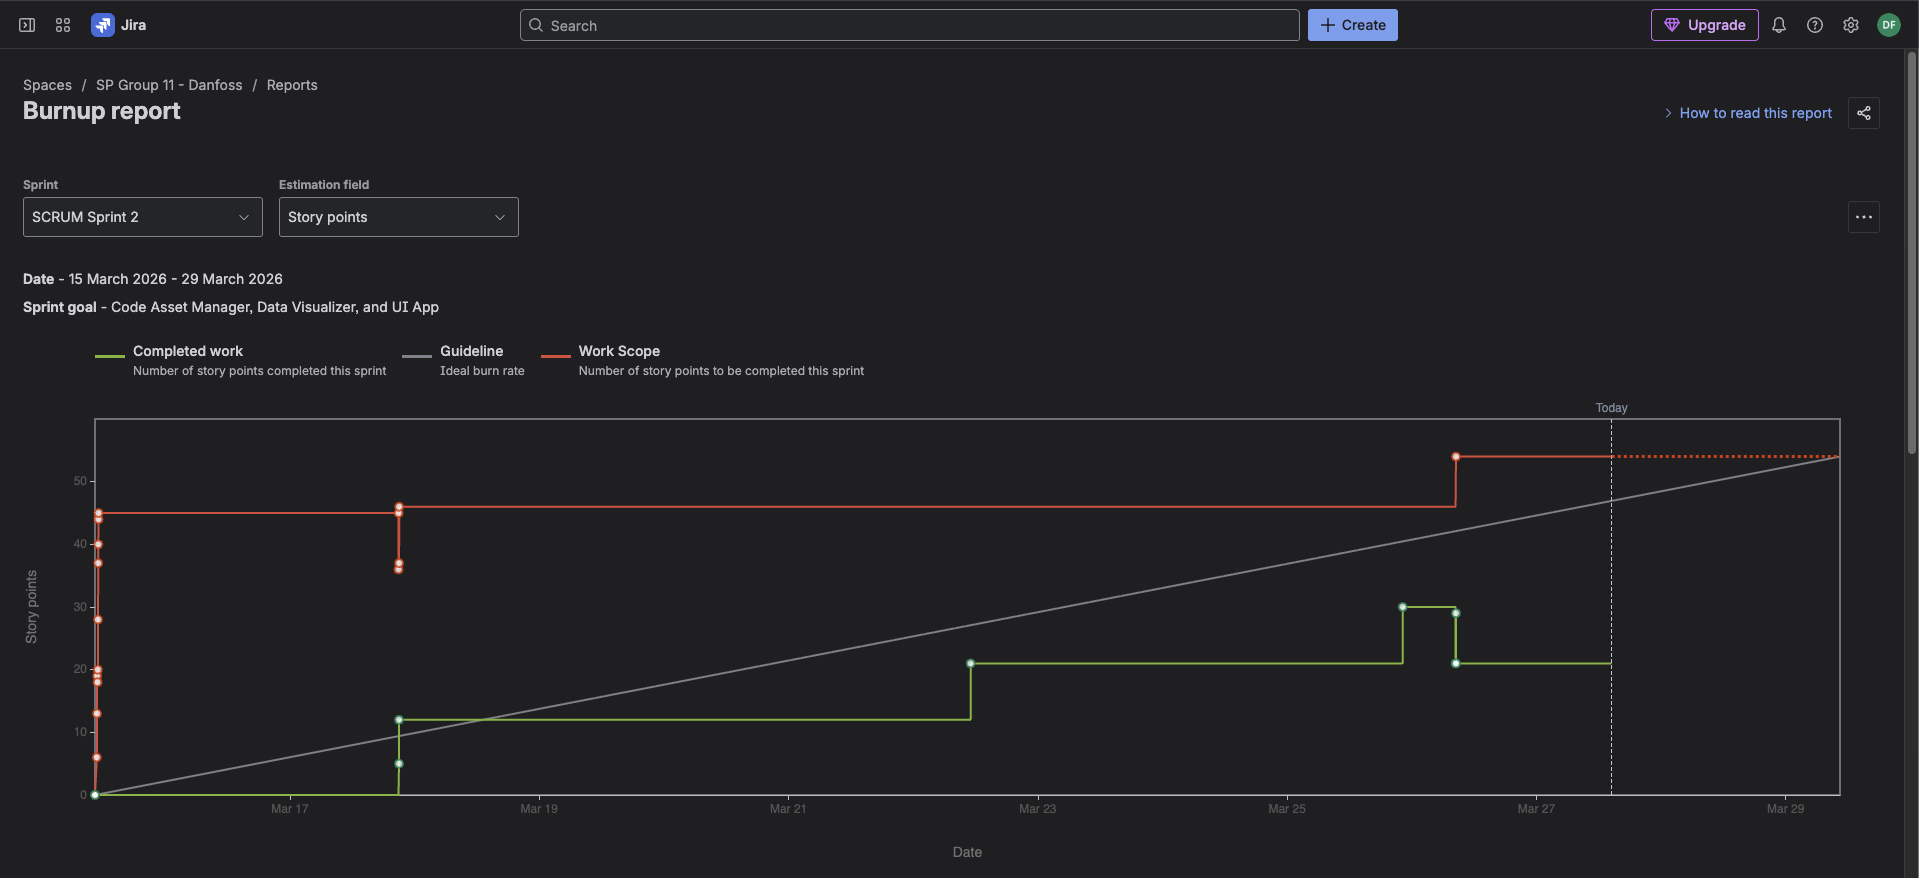
\includegraphics[width=0.95\textwidth]{sprint2-burndown-jira.png}
    \caption{Sprint 2 burndown chart.}
    \label{fig:sprint2-burnup}
\end{figure}

% =============================================================
\section{Sprint 3}
\label{sec:sprint3}
% =============================================================

Sprint 3 focused on the remaining modules which were the Optimizer, the Result Data Manager and the Data Visualizer. Zoja Angelovicova acted as the Scrum Master and Dominik Bezo as the Meeting Coordinator, while Pavel Seliavko transitioned into the role of internal Product Owner. To address the mid-sprint creation and replacement of the tickets, a problem identified in Sprint 2, the planning style was changed. Each pair created its own detailed subtickets for the assigned module before starting with the development. To address the burndown chart inaccuracies encountered in Sprint 2, each subtask was logged as an individual ticket to ensure accurate progress tracking in Jira (see Appendix~\ref{sec:appendix-backlogs} Fig.~\ref{fig:sprint3-backlog-start}).

Additionally, pair-programming assignments were reorganised to ensure greater schedule compatibility among team members:
\begin{itemize}
    \item Maria Tsioni and Dominik Bezo
    \item Zoja Angelovicova and Daniel Falat
    \item Pavel Seliavko and Zoe Elea Schiwy
\end{itemize}

Sprint 3 successfully delivered a functioning Optimizer, Result Data Manager, and Data Visualizer. However, integration errors encountered during the merging of parallel branches required the sprint deadline to be extended from April 16th to April 19th. As a result, several tickets remained incomplete at the originally planned end of the sprint (see Appendix~\ref{sec:appendix-backlogs} Fig.~\ref{fig:sprint3-backlog-16apr}). The conflicts were resolved by a full team merge. All of the branches were merged into a single branch \texttt{SCRUM-81-Version-1}. Furthermore several tickets had to be renamed to reflect what had actually been implemented.

The Retrospective used a \textsc{Start} / \textsc{Stop} / \textsc{Continue} board with silent writing and round-robin sharing methods (see Appendix~\ref{sec:appendix-backlogs} Table~\ref{tab:sprint3-retro}).

% =============================================================
\section{Sprint 4}
\label{sec:sprint4}
% =============================================================

The primary objective of the Sprint 4 was to finalise and test the product. The nature of the tasks in this sprint was better suited to two groups of three members rather than three pairs. This reorganisation was carried out in accordance with the recommendation made during the previous Sprint Retrospective:
\begin{itemize}
    \item \textbf{Team Slovaks} -- Daniel Falat, Dominik Bezo and Zoja Angelovicova
    \item \textbf{Team International} -- Maria Tsioni, Pavel Seliavko and Zoe Elea Schiwy
\end{itemize}

Daniel Falat took the Scrum Master role and Dominik Bezo took the role of the Meeting Coordinator. Planned work included switching between scenario 1 and scenario 2, refactoring of the Optimizer, removing redundancy in the TimeSeries, implementing maintenance selection, updating the Result Data Manager headers, applying the UML feedback from the lecturer, and writing unit, functional and integration tests for every module. Time estimation and the time actually spent was also added to the tickets for the first time.

Because the focus was heavily directed at making the technical product fully working the tickets regarding report-writing originally planned for this sprint had to be returned to the backlog at the end of the sprint (see Appendix~\ref{sec:appendix-backlogs} Fig.~\ref{fig:sprint4-completed} and Fig.~\ref{fig:sprint4-incomplete}).

The primary issue of the sprint surfaced during the Task Review: the two teams had independently produced very similar solutions for different tasks (SCRUM 117 \& 118 and SCRUM 128 \& 131), creating duplicate code. The conflict was resolved through a discussion between the whole team where it was decided that for documentation reasons, the best resolution was to keep the duplicate implementation while only keeping one solution active. By the Sprint Review on the 1st of May the Minimum Viable Product was complete and verified through testing. Report writing had to be transferred to Sprint 5. The team determined that a comprehensive Start / Stop / Continue retrospective was not warranted this sprint, as collaboration within both teams had functioned effectively.

% =============================================================
\section{Sprint 5}
\label{sec:sprint5}
% =============================================================

Sprint 5 focused mainly on the division of the report tasks, report-writing and refactoring of the code. Because of the Math 2 exam on the 8th of May, a thorough Sprint Planning meeting was held before that on the 3rd of May. The sprint was formally started on the 9th of May, with the end date moved to the 17th of May. Maria assumed the role of Scrum Master and Zoja the Meeting Coordinator, Pavel continued to be the Product Owner. The team composition established in Sprint 4 was retained, maintaining the same two groups of three members (see Appendix~\ref{sec:appendix-backlogs} Fig.~\ref{fig:sprint5-backlog-start}).

On the development side, Team Slovaks was responsible for ensuring the Data Visualizer called Optimizer only once with a clearer separation of concerns, and Team International took the refactoring of the Unit models to use more abstraction/inheritance and fewer interfaces. For the report, every chapter was assigned to an individual author and reviewer (see Table~\ref{tab:report-responsibilities} in Appendix~\ref{sec:report-responsibilities}), except for Chapter 5 which is the Implementation. This chapter is jointly authored by both teams. A dedicated meeting was scheduled for the 16th of May to produce the final Class, Activity and Sequence diagrams used in the report.

During the Sprint Review and Retrospective, no major issues were identified. However, the report-writing tasks had to be carried over to the next sprint, with the tickets already being in progress.

% =============================================================
\section{Sprint 6}
\label{sec:sprint6}
% =============================================================

Sprint 6 was the final sprint of the project, scheduled from the 18th of May to the 1st of June. It was set to be longer than the previous ones because it had to cover the last round of code changes, writing of the remaining report chapters and the full review cycle before the submission deadline.

The two teams from Sprint 4 and 5 were kept, but the team structure was only used for the shared Implementation chapter. The rest of the report writing was assigned per chapter, with a dedicated reviewer for each one. Zoe Elea Schiwy assumed the role of the Scrum Master, Daniel Falat the role of Meeting Coordinator, and Pavel Seliavko remained the Product Owner.

The sprint goal was \enquote{Finish the Report and change the code based on the feedback from Danfoss}. The code-related part of the goal followed from the final demonstration with Danfoss representatives, during which three concrete points were raised: the ratio used in the Optimizer had to be adjusted, and the legend and colours in the Data Visualizer had to be corrected. These were tracked as SCRUM-170, SCRUM-171 and SCRUM-173.

Additional feedback was received from lecturer Amir Ghomashi and distributed across the existing report-writing tickets rather than turned into a separate ceremony. No major conflicts arose during Sprint 6, and the Sprint Review and Retrospective were planned for the day before the submission deadline.                                       % Call file with chapter

% -------------------------------------------------------------
% SOLUTION
% -------------------------------------------------------------
\chapter{Solution}                                             % Chapter title
\label{chap:solution}                                          % Chapter label

%----------------------------------------------------------------------------------------
%    Solution
%----------------------------------------------------------------------------------------
\section{UML Diagrams}
\subsection{Activity Diagrams:}
\begin{figure}[h]
    \centering
    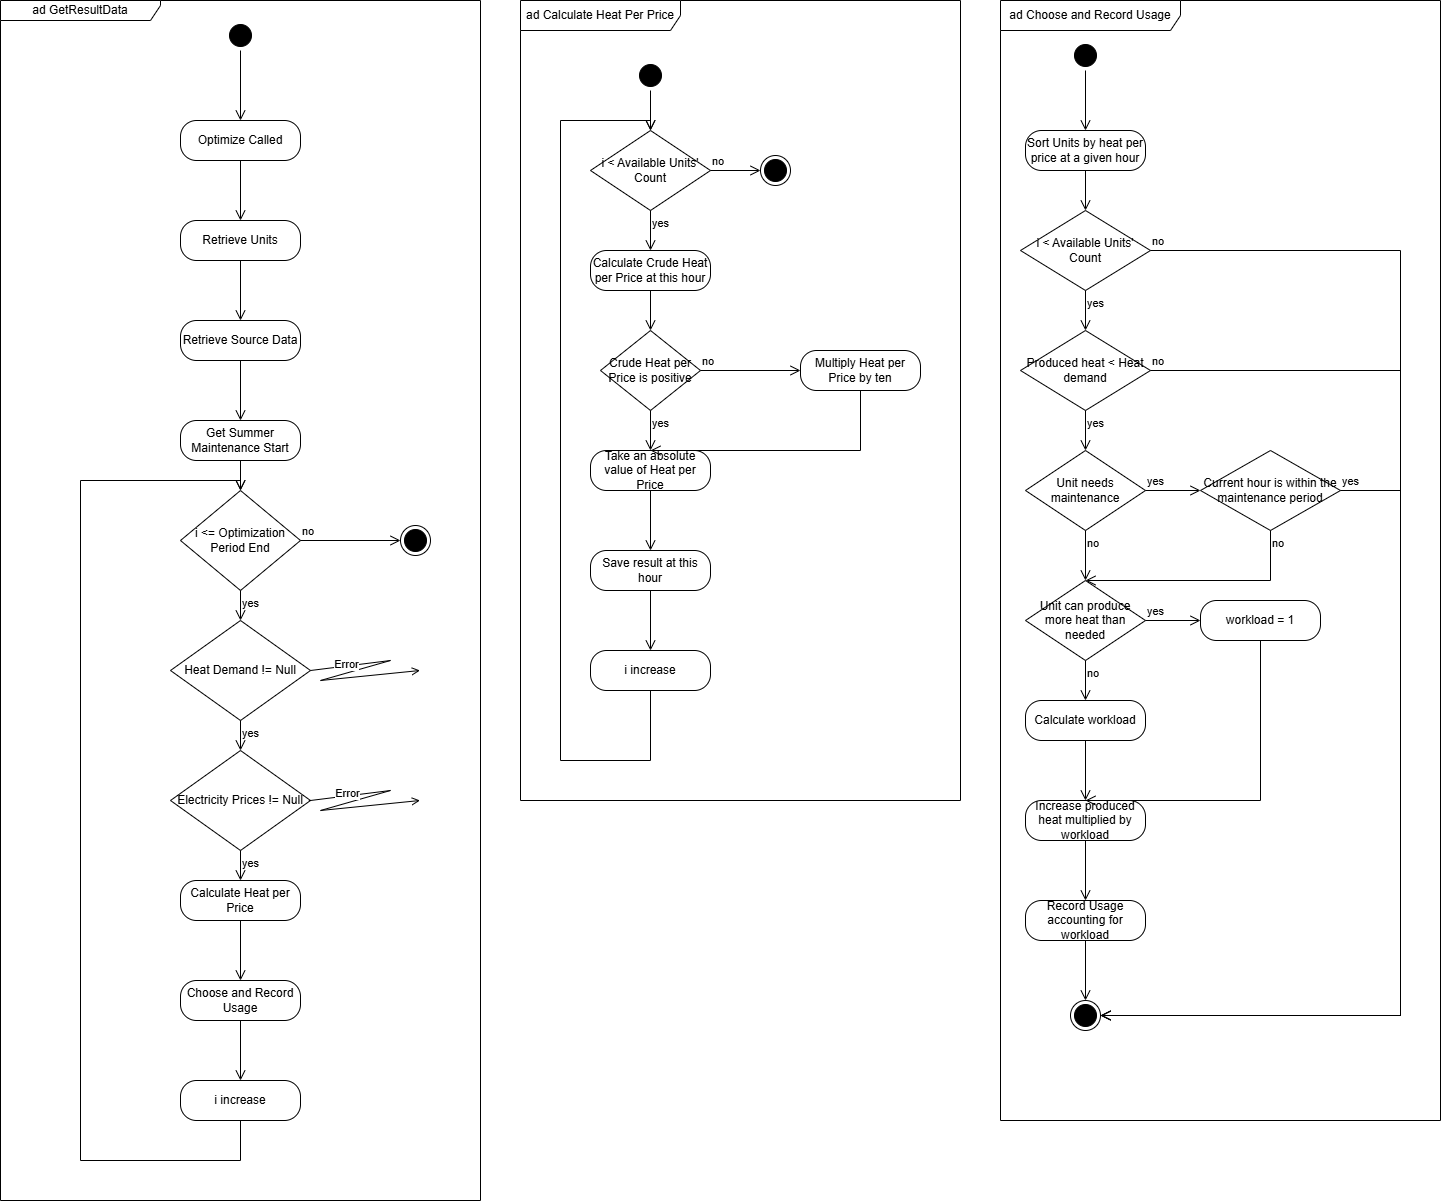
\includegraphics[width=1\textwidth]{ActivityDiagram.png}
    \label{fig:ActivityDiagrams}
\end{figure}
\noindent These diagrams represent the optimization algorithm. The process happens inside the optimizer class, it starts when the GetResultData method of the optimizer is called. That calls the Optimize method, which proceeds to retrieve all data necessary for optimization to commence. 

\noindent When data has been gathered it enters a loop, going through every hour of every day of the optimization period. In the loop it checks if the gathered data is workable, after, if data is correct, the process continues. The weighted ratio of heat to price of each unit is calculated, then the optimal unit is selected to be used in heat production and usage is recorded. This happens on a per hour basis by calling CalculateHeatPerPrice and ChooseAndRecordUsage methods.

\noindent CalculateHeatPerPrice method loops through the units, for each unit the ratio is calculated by first getting a crude heat divided by price, then the crude ratio is weighted by a factor of ten if it is negative. The weighting is performed to increase the unit's priority, because negative heat per price means that the unit is making money instead of costing money. 

\noindent The ChooseAndRecordUsage method first sorts units by their heat per price ratio. When the list is sorted it enters a loop going through the sorted list, keeping track of heat demand, how much heat has been produced and how many units are available. Loop stops if it runs out of units or if the heat demand is reached. At the start of the loop it checks if the current unit is on maintenance, if unit is on maintenance it is skipped, otherwise loop proceeds. The next step is to check if the unit's maximum heat production exceeds remaining heat demand, which is the difference of total heat demand and produced heat. This is done to calculate workload - a coefficient from 0 to 1 that represents how much unit is used. If heat production is not exceeded the workload is 1, otherwise it is calculated by dividing remaining heat demand by the current unit's maximum heat production. After calculating workload, produced heat is increased by current unit’s maximum heat production multiplied by workload, and then all unit’s relevant characteristics, such as pollution, heat, fuel consumption, are recorded multiplied by workload.

\subsection{Sequence Diagram:}
\begin{figure}[h]
    \centering
    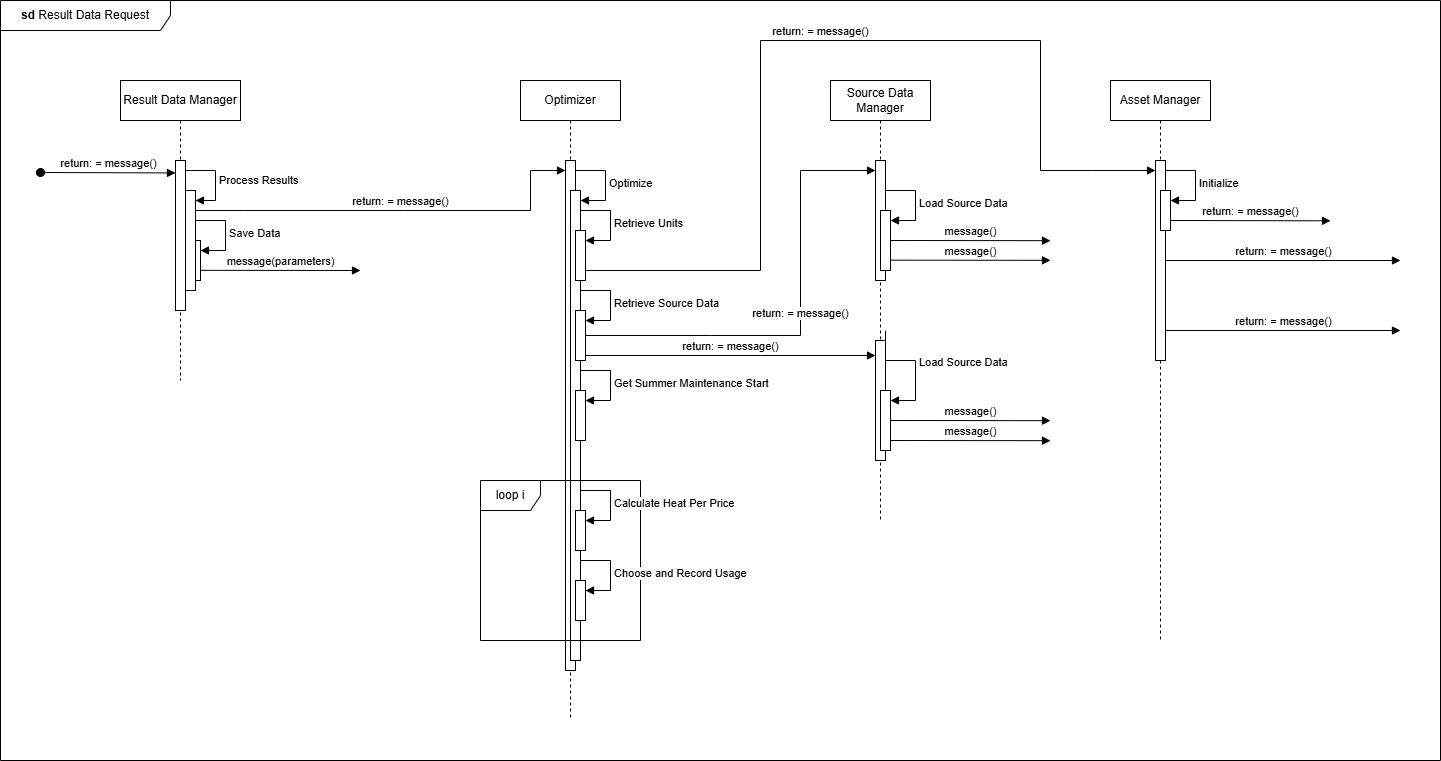
\includegraphics[width=1\textwidth]{SequenceDiagram.png}
    \label{fig:SequenceDiagram}
\end{figure}
\noindent This sequence diagram represents how service classes interact when result data is requested.

\noindent Requests can come from several parts of the Presentation layer, which is represented as a found message.

\noindent The Result Data Manager makes a self-call, which then calls Optimizer. After that is resolved, within the same self-call another self-call is made to save Optimization results in local .csv files. For data management a call to a separate class is made, represented as a lost message. After that, the Result Data Manager’s sequence ends. 

\noindent The Optimizer makes a self-call that then makes three self-calls, first resulting in a call to the Asset Manager and second in two calls to the Source Data Manager. It then enters a loop of two self-calls. After that Optimizer’s sequence ends.

\noindent The Asset Manager makes a self-call to initialize. Initialization uses a separate class for data management, this is represented as a lost message. After that is resolved Asset Manager uses two separate classes to provide the correct scenario, and units of correct classes - those are represented as lost messages. After that Asset Manager’s sequence ends.

\noindent Source Data Manager sequence starts when it receives the first call from Optimizer. This results in a self-call that uses a separate class for data manipulation represented as two lost messages. Then a second call from the optimizer results in following the same sequence. After that Source Data Manager’s sequence ends.

\subsection{Class Diagram:}
\begin{figure}[h]
    \centering
    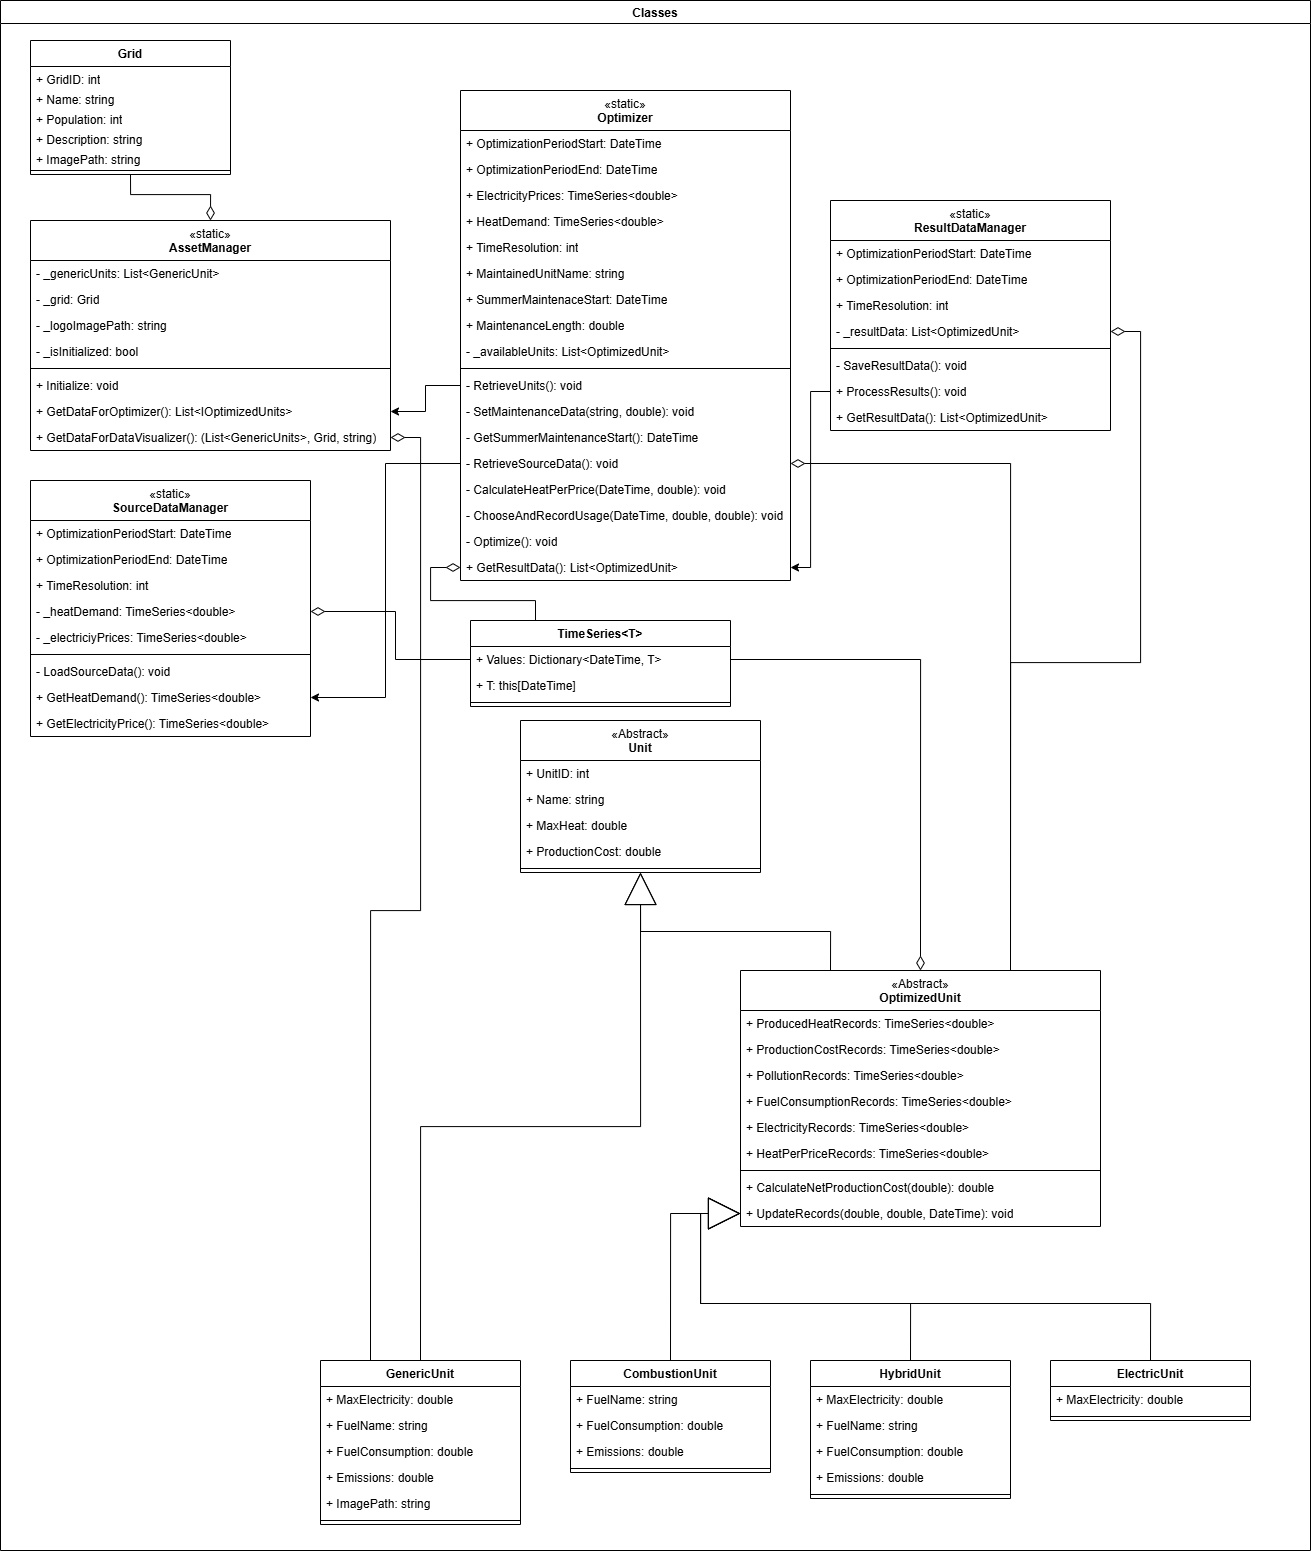
\includegraphics[width=1\textwidth]{ClassDiagram.png}
    \label{fig:ClassDiagram}
\end{figure}
\noindent This class diagram represents the core of the solution: services and models.

\noindent AssetManager has a one-way association with the Optimizer. This one-way association shows that AssetManager is called by the Optimizer, but doesn’t call it. AssetManager aggregates instances of GenericUnit and Grid. This aggregation relationship shows that those are independent concepts.

\noindent SourceDataManager has a one-way association with the Optimizer. This shows that Optimizer can call SourceDataManger, but SourceDataManager doesn’t call Optimizer. It aggregates the TimeSeries<T> class. This represents that TimeSeries<T> is an independent class.

\noindent Optimizer has one-way associations with AssetManager, SourceDataManager and ResultDataManager. Those represent that Optimizer calls AssetManager and SourceDataManager, but is not called by them. And that shows that Optimizer is called by ResultDataManager, but doesn’t call it. Optimizer aggregates TimeSeries<T> and OptimizedUnit. The aggregation relationship shows that both are independent concepts.

\noindent ResultDataManager has a one way association with the Optimizer. This shows that Optimizer is called by ResultDataManager, but ResultDataManager is not called by Optimizer. ResultDataManager  aggregates OptimizedUnit. This aggregation relationship shows that this is an independent class.

\noindent Unit models form an inheritance tree. GenericUnit class and abstract OptimizedUnit classes inherit from the base abstract class Unit. GenericUnit represents units with characteristics including an image, while OptimizedUnit represents units with only performance specifications, and records of usage. From the abstract OptimizedUnit class three classes: CombustionUnit, HybridUnit and ElectricUnit, inherit to allow for the differences in how they calculate price and how they record usage.

\section{Technical Architecture}
\noindent Project was coded in C\# in .NET framework, using Avalonia UI in combination with OxyPlot, ReactiveUI and CommunityToolkit.Mvvm for Data Visualization. All input and output data, specifically: images, units' specifications and resulting schedule are stored locally, file manipulation is performed by use of System library and CsvHelper library. Tests were implemented in the xUnit framework.

\noindent Solution is separated in following layers:
\begin{itemize}

    \item [\(\cdot \)] Data Handling
    \begin{itemize}
        \item [\(\circ \)] Data
        \item [\(\circ \)] Assets
    \end{itemize}
    \item [\(\cdot \)] Business Logic
    \begin{itemize}
        \item [\(\circ \)] Models
        \item [\(\circ \)] Services
        \item [\(\circ \)] ViewModels
    \end{itemize}
    \item [\(\cdot \)] Presentation
    \begin{itemize}
        \item [\(\circ \)] Views
    \end{itemize}

\end{itemize}
\noindent The project's architecture is a combination of the MVVM pattern and micro-service architecture approach.

\noindent Data Handling layer includes: Data - classes that handle file manipulation; Assets - static data storage consisting of .json, .csv and .png files.

\noindent Business Logic includes: Models - classes that: model real life objects and concepts, transfer data, represent UI components; Services - classes that manage classes from Data, and control the process of optimization; ViewModels - classes that provide functionality to the UI and establish connection between Models, Services and Presentation layer.

\noindent Presentation layer includes: Views - partial classes that control the appearance of the UI.

\noindent This structure was chosen because it follows SOLID principles which facilitate flexibility and scalability, by significantly reducing required amount of refactoring in development process. MVVM pattern was implemented in the overall structure of this project. Core benefit of MVVM is separation of responsibilities. Microservice architecture is most represented by Services and it follows the Open/Closed principle.
                                      % Call file 

% -------------------------------------------------------------
% IMPLEMENTATION AND TECHNICAL REALIZATION
% -------------------------------------------------------------
\chapter[Implementation]{Implementation and Technical Realization}
\label{chap:implementation}

% -------------------------------------------------------------
%    Implementation
% -------------------------------------------------------------

\section{Implementation}
\subsection{Implementation Frontend}

\subsubsection{Architecture and Technology Stack (MVVM in Avalonia UI)}
\label{sec:architecture-mvvm-avalonia}

The client application is built on the .NET platform using the Avalonia UI framework. Avalonia was chosen for its consistency with the Advanced Object-Oriented Programming course curriculum. The layout is described in XAML, so the structure of the interface is kept in markup files and the C\# code-behind only contains what cannot be expressed declaratively.

The internal structure follows the Model--View--ViewModel (MVVM) pattern. MVVM was selected because the user interface and the optimization logic had to be developed in parallel by two sub-teams, and the pattern enforces a clear boundary between them. Keeping the View independent from the optimization code also made it possible to test the ViewModels in isolation, without instantiating any Avalonia controls. The three layers are organised as follows:

\begin{itemize}
    \item \textbf{View:} The interface is defined in \texttt{MainWindow.axaml}. The file contains only XAML --- layouts, styles, themes and bindings to the corresponding ViewModels. Its code-behind, \texttt{MainWindow.axaml.cs}, is intentionally kept minimal and only handles operations that cannot be expressed through bindings, such as loading the logo asset and switching between the application's pages.

    \item \textbf{ViewModel:} \texttt{MainWindowViewModel.cs} acts as the root ViewModel and owns the nested ViewModels used by the rest of the application. The two main ones are \texttt{DataVisualizerViewModel.cs}, which holds the state and configuration of the interactive charts, and \texttt{UnitViewModel.cs}, which exposes the parameters and operational constraints of an individual heat production unit to the View.

    \item \textbf{Model:} The data layer is represented by the \texttt{DataVisualizerModel.cs} class, which contains time series data, data on previous operations, and data from the optimizer. This class provides access to the data needed for further visualization in the form convenient for use in the ViewModels.
\end{itemize}

Interaction between all three layers in the architecture is provided via the ReactiveUI library. The observable properties of both Models and ViewModels are created using the \texttt{RaiseAndSetIfChanged} method, which raises the property changed event each time the corresponding value changes. Thus, any change in the View, such as changing the slider to maintain a particular heat-producing unit, changes the value in the ViewModel that in turn recalculates the results of the Optimizer and the plot. Therefore, there is no need to explicitly call refreshing in the View.

% DOMINIK
% put your chapters here
\subsubsection{UI Elements and Styling}
The layout of the on-screen UI Elements was designed with the main objective being availability of all functionalities at one place. The operator has access to everything that the system is capable of executing,
from scenario switching, through period switching, to maintenance planning. The entire interface is defined in the MainWindow.axaml file, and it is structured and contained in a Grid container.

The left section - the \textbf{Control Panel} - consists of a dark-red column, 2 radio buttons, slider bar, dropdown menu, and a theme toggle switch. It uses the dark-red coloured background because it is the characteristic color of the \textit{Danfoss} company.
\begin{enumerate}
    \item \textbf{Scenario Switch} - It is built using two rounded radio buttons with the \texttt{GroupName} being "ScenariosGroup". It allows the operator to switch between the Scenario 1 (Heat Scenario)
    and Scenario 2 (Heat \& Electricity Scenario). After selecting an option, the graph in the main section of the frame automatically updates and shows the selected option, either the Heat Scenario
    or the Heat \& Electricity Scenario. The IsChecked binding of this switch is connected to the \texttt{IsHeatScenarioSelected} and the \texttt{IsHeatAndElecScenarioSelected} attributes inside the
    \texttt{MainWindowViewModel.cs} file.
    \item \textbf{Period Switch} - It is also built using two rounded radio buttons with the \texttt{GroupName} being "PeriodGroup". This switch allows the operator to switch between the Summer Period
    and the Winter Period. After selecting an option, the graph in the main section of the frame automatically updates and shows the selected option, either the Summer Period or the Winter Period.
    The \texttt{IsChecked} binding is connected to the \texttt{IsWinterSelected} and the \texttt{IsSummerSelected} attributes inside the \texttt{MainWindowViewModel.cs} file.
    \item \textbf{Maintenance Planning} - Section for scheduling the maintenance period, for time selected using the slider, and for the selected production unit from the dropdown menu. The slider value
    ranges from 30 to 60 hours. In addition, the slider has snapping allowed with the \texttt{TickFrequency} being set to 1. There is a text label under the slider, that is bound to the slider value.
    Furthermore, there is a \texttt{ComboBox} dropdown menu under the text label, containing every production unit available, with the option "None" as well, in case there is no maintenance needed for
    scheduling. The \texttt{SelectedItem} is binded to the \texttt{SelectedUnit} attribute inside the \texttt{MainWindowViewModel.cs} file.
    \item \textbf{Theme Toggle} - A toggle switch located at the very bottom section of the Control Panel sidebar controlling \texttt{IsDarkTheme} and switching the entire system theme.
\end{enumerate}

The right section - the \textbf{Main Section} - consists of 3 vertical areas:
\begin{enumerate}
    \item \textbf{Header} - It consists of a text label stating the official name of the tool, the location/city where the heat distribution is operated at, and the approximate number of buildings in the
    district heating area. In addition, there is a \textit{Danfoss} logo, loaded from the application assets, located at the very right section of the Header.
    \item \textbf{Interactive Chart} - The most important part of the screen. It contains an \texttt{oxy:PlotView}, which is bound to \texttt{Visualizer.CurrentPlotModel}. Below the chart, there is a horizontal
    panel with checkboxes for selecting the metrics to be displayed on the chart, namely: Heat Demand, Heat Production (these two are set to \texttt{IsChecked} as default), Electricity, Electricity Price (these
    two are only available to be selected when operating in the Scenario 2 - the Heat \& Electricity Scenario), CO\textsubscript{2} Eimissions, Fuel Consumption, and the Production Costs). In addition, there
    is a Legend button located in the bottom-right corner of this section, which when clicked expands and displays a detailed pop-up legend, explaining which color on the graph represents what metric.
    \item \textbf{Production Units Cards} - A responsive \texttt{UniformGrid} with three columns, located at the very bottom of the screen below the \textbf{Interactive Chart} section, displaying detailed
    specification of three production units at once. There are arrows located on both left and right side of this section, allowing the operator to navigate between all available production units which are paginated,
    allowing the system to create a new page of production unit cards, in case a unit, or multiple units were added.
\end{enumerate}

To ensure a proffesional interface, there were multiple overrides defined for the \texttt{ControlTemplate} in \texttt{Window.Style}, inside the \texttt{MainWindow.axaml} file. The traditional radio buttons were transformed into a more modern segmented buttons. The following XAML code snippet defines the right-rounded radio button segment with a checkmark visible only when selected:

\begin{figure}[H]
    \centering
    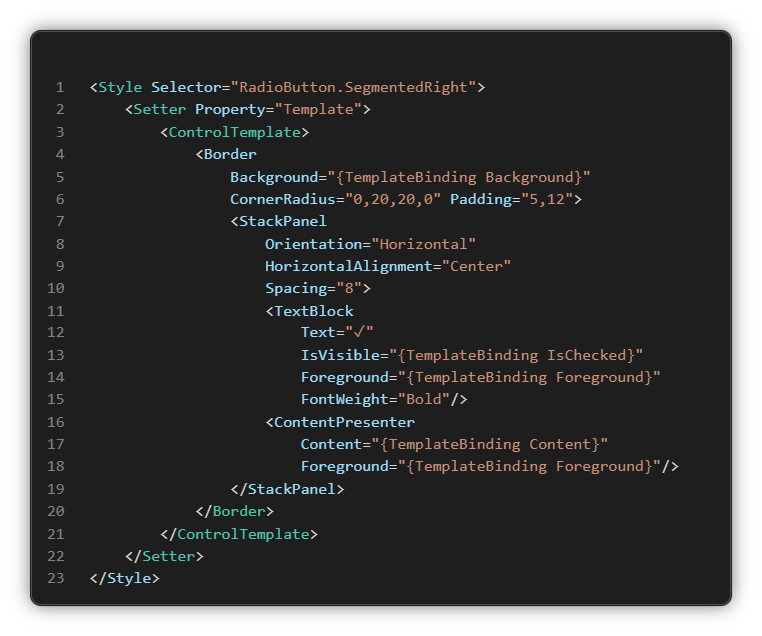
\includegraphics[width=1\textwidth]{Images/RadioButtonStyle.png}
    \caption{Radio Button with Visible Checkmark}
    \label{fig:radiobutton}
\end{figure}

The combo box for selecting production units for maintenance scheduling is also visually customized to have dark-red background, white text, and both hover and selection states.

\begin{figure}[H]
    \centering
    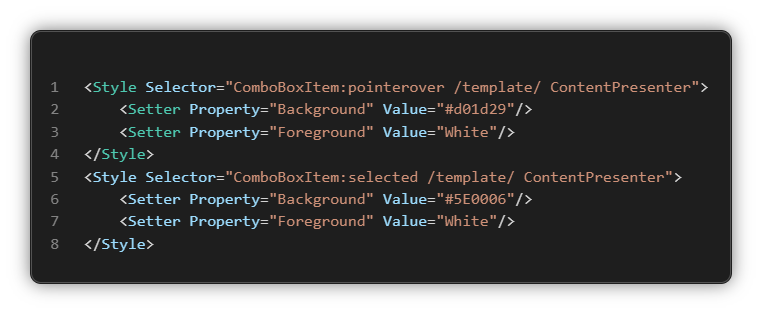
\includegraphics[width=1\textwidth]{Images/ComboBoxStyle.png}
    \caption{Combo Box Style Configuration}
    \label{fig:combobox}
\end{figure}

The production unit cards at the very bottom of the right section are modified rectngular modules (\texttt{CornerRadius="15"}, \texttt{ClipToBounds="True"}). There is the image of the
production unit on the left side of the card, which is loaded from the application assets, and will automatically adapt to the size of the card via \texttt{Stretch="UniformToFill"}.
Lastly, there are specification and different metrics that are significant to each production unit available, and they are shown on the right side of the card. This part of the card is
designed to have dark-red background and white text, which ensures perfect readability even when using lower screen resolutions.

\subsubsection{UI Logic and Engineering Decisions}

\subsubsection{Data Flow}
During the architecture design phase, the main goal of the team was to clearly separate the presentation layer (frontend) from the complex mathematics of the optimisation algorithms (backend). This was achieved by implementing a strict data flow structure.

\begin{enumerate}
    \sloppy
    \item \textbf{Initialisation} 
    
    After the app is launched, \texttt{MainWindow}\allowbreak\texttt{ViewModel} becomes the most important class, since it essentially controls the app flow. This ViewModel requests a list of all available production units using the Asset Manager's \texttt{AssetManager.}\allowbreak\texttt{GetDataForDataVisualizer()} method. In order for the app to load quickly and remain smooth, the \texttt{AssetManager} class is designed to cache all loaded data. When the app is launched for the first time, it uses the \texttt{AssetsLoader} class to read and parse the data from JSON files. Whenever the \texttt{AssetManager} is called again, it does not need to read the data from disk, but rather returns the data directly from the cache. This approach helps to decrease latency as much as possible and ensures that the UI loads more quickly, even with a growing number of production units.

    \item \textbf{Optimisation} 
    
    The optimisation data cycle begins whenever the operator uses the control panel to change the configuration. It can be initiated by either changing the scenario, switching the optimisation period between summer and winter, or adjusting the maintenance settings.
    
    \begin{itemize}
        \item \texttt{MainWindow}\allowbreak\texttt{ViewModel} detects changes in the configuration and launches the \texttt{RefreshData}\allowbreak\texttt{AndChart()} method. This method handles synchronisation of the scenario configuration using the \texttt{ScenarioManager.}\allowbreak\texttt{CurrentScenario} method. Afterwards, the \texttt{SyncOptimization}\allowbreak\texttt{Period()} method is called, which defines clear time boundaries for both the winter and summer periods. The summer period ranges from 8 September to 22 September, while the winter period ranges from 5 January to 19 January. Maintenance settings are sent to the Optimizer module using the \texttt{Optimizer.}\allowbreak\texttt{SetMaintenanceData()} method.
        \item After all configuration data is saved, \texttt{MainWindow}\allowbreak\texttt{ViewModel} instructs \texttt{DataVisualizer}\allowbreak\texttt{Model} to update the data using \texttt{Visualizer.}\allowbreak\texttt{Model.}\allowbreak\texttt{UpdateData()}. At this stage, \texttt{DataVisualizer}\allowbreak\texttt{Model} requests data from \texttt{ResultData}\allowbreak\texttt{Manager}, which starts the optimisation process. The goal of the optimisation is to meet the heat demand using the available production units. The \texttt{Optimizer} calculates workload and then selects the most profitable configuration of units to activate.
        \item When the optimisation process is complete, \texttt{ResultData}\allowbreak\texttt{Manager} saves the result data into CSV files using the \texttt{SaveResultData()} method. These records serve as a debugging tool if the optimisation does not run correctly or for occasional audits.
        \item In the end, the \texttt{DataVisualizer}\allowbreak\texttt{Model} receives the result data in form of \texttt{OptimizedUnit}. It prepares the data for the \texttt{DataVisualizer}\allowbreak\texttt{ViewModel}, where the resulting \texttt{TimeSeries} data are converted into curves and bars on the chart. The \texttt{UpdatePlot()} method links units with the correct colours from \texttt{ChartColors.cs}, sets up axes using \texttt{Axes.cs}, the legend using \texttt{Legend.cs}, and calls \texttt{InvalidatePlot(true)} to ensure that the updated graph is displayed immediately within the GUI.
    \end{itemize}
\end{enumerate}

\vspace{1em}
\noindent\textbf{Conclusion of the Data Flow}

\noindent Due to this strictly engineered data architecture, the entire 14-day optimisation, including exporting data into CSV files and rendering of complex graph usually takes less than 100 milliseconds. The operator therefore receives immediate feedback which ensures a fluid and positive user experience.

   

% -------------------------------------------------------------
% DISCUSSION AND REFLECTION
% -------------------------------------------------------------
\chapter{Discussion and Reflection}
\label{chap:discussion} 

% =============================================================
%    Chapter 6: Discussion and Reflection
% =============================================================

\section{Scrum}
During the development of the project, a Scrum agile was implemented to deliver structured and transparent software development. Over the semester, six sprints were completed. Each sprint contributed to the team’s development, working methods, and the quality of the final semester project.

\subsubsection*{Reflection on Scrum practices and their benefits}
Transparency and responsibility were ensured by rotating the role of Scrum Master each sprint (Dominik in S1, Pavel in S2, Zoja in S3, Daniel in S4, Maria in S5, Zoe in S6). This allowed each team member to take responsibility for all processes and sprint coordination. Using Jira provided a clear overview of task status, with each ticket having a clearly defined assignee or team and a reviewer to ensure quality.

In the first sprint, the workload distribution was underestimated. As a solution, a story points system was introduced, using a scale of 1–10 based on the sum of difficulty (1–5) and importance (1–5). This system greatly improved our planning and monitoring of burn-down charts. Later, also deadlines for tasks were used to help review them on the go, so that there always was enough time to fix issues the development team or pair might have missed.

Throughout the development phase, team and pair programming were utilized. The first three sprints were pair-based, with pairs changed twice. In sprints 4–6, workload was divided between 2 teams of three (team Slovaks and team Internationals). This technique proved effective and helped us eliminate technical problems from the early sprints, particularly those related to time management.

\subsubsection*{Observed changes in behaviour and code quality}
By implementing code reviews and coding principles in the second sprint, a higher consistency was reached, also a cleaner and easier-to-read code was produced to help understand everything for those who had not written that part.

After facing difficulties in the initial phase such as missing feedback from each other during meetings and passivity, the team implemented a rule to use webcams. This solution also proved to be effective and improved the sense of presence and teamwork.

\subsubsection*{Difficulties and issues}
During the development, the team faced several issues, for example, in Sprint 2, tickets needed to be added in the middle of the process because the technical difficulty was not estimated correctly. Team’s response was implementing more detailed sprint planning, dividing large and important tasks into smaller tickets that were more predictable.

Duplicity and assumptions were also challenges that were faced. In the fourth sprint, miscommunication and assumptions led the team to produce the same part of the code twice. This experience was very beneficial for learning and implemented stricter coordination between the Slovak and International teams in the later phase of project development.

During development, the team experienced issues with Jira, where tickets were sometimes not marked as done even after being moved to the ``Done'' column. This was later fixed, but the charts still did not reflect reality. There was another issue – the presence of subtasks within each ticket. It was addressed by transitioning to separate tickets in order to have the chart displayed correctly. Despite these solutions, the chart remained problematic although it was more realistic than in the beginning.

\section{Requirements Engineering}
The engineering process in the project was important in transforming the task into functional and professional software. This process helped maintain the correct scope of the user requirements and the technical implementation of the solution.

\subsubsection*{Impact of adopted practices on work quality}
In the beginning, a noun-verb analysis was conducted. This technique helped in the early development stage by identifying important entities and their desired behaviour. As a result, the key responsibilities of each module (for example, Asset Manager, Source Data Manager) were precisely defined, which led to a clearer architecture and separation of concerns.

Creating the product backlog based on user stories helped with dividing the complex system into smaller, more testable functions. This ensured that during the development we remained focused on our goal: optimising heating expenses.

Before starting application development, the UI was prototyped. Each team member sketched their vision of the UI, after which the best design was picked and then improved by incorporating better ideas from other sketches. After creating final sketch, a proper Figma prototype for the GUI was created, which served as source of truth for UI. This process eliminated uncertainties in front-end development with Avalonia and saved time otherwise spent discussing design.

A decision to use UML diagrams and CRC cards as dynamic documents that evolved with the code development enabled the team to react more flexibly to new discoveries during implementation.

\subsubsection*{Important takeaways for future projects}
In the future, it would be beneficial to keep the practice of reconsidering requirements in the beginning of each sprint. For example, in the second sprint it was discovered that in order to solve Data Visualizer module, a Source Data Manager had to be developed prior, which helped prevent blocking the progress of other teams.

Another takeaway is collaboration with Product Owner. During development, it proved to be necessary for clearing up uncertainties in some tickets. In the future team would plan to use this role even further and more intensively in agreeing acceptance criteria in certain tasks and in avoiding assumptions.

\section{Refactoring}
Refactoring in our project was one of the key processes, which continued in parallel with the development of new application features. Its goal was not only to clean up the code, but also to keep the code more maintainable and readable when different teams worked on the same parts of the project.

\subsubsection*{Effects of refactoring on our code quality}
As mentioned in 6.1, a set of strict coding principles was developed, which were later applied in each refactoring. These principles mainly included reducing nesting to a maximum of 3 layers and extraction of duplicate code into separate methods.

The most important phase of refactoring occurred in Sprints 4 and 5, where after merging branches, the team had to clear up redundancies in TimeSeries which enabled easier data access and processing across different modules. We also refactored DataVisualizerViewModel for better maintainability and made changes to interfaces which were removed and the code was simplified with the same functionality.

\subsubsection*{Skills balance and teamwork}
Refactoring was used as a tool to balance technical skills across group. Through the pair programming, less experienced members were able to learn best practices and coding standards from their peers while working on code clean-up.

Rotating work between teams, for example having Team Slovaks refactor modules initially developed by Team International, ensured that everyone understood overall architecture rather than just single module.

Furthermore, establishing the English as standard for all comments and naming (after listening to feedback from each other based on previous semester project) during our refactoring sessions significantly improved collaboration and understanding within an international team.

\subsubsection*{Challenges during refactoring}
One of biggest challenges was keeping our documentation in sync with the code. As project evolved, UML diagrams and CRC cards had to be constantly updated to reflect latest refactored state, which was demanding to manage alongside development.

Another significant hurdle that was encountered was that the code was written in quite complicated way, even though it followed the coding principles that were agreed on. This complexity meant that the refactoring took much more time than initially expected. The team had to spend the extra effort to simplify the logic and make it more readable without breaking any of functionality we already implemented.

\section{Code review}
Code review was a necessary step before merging changes into active development branches (for example, ``Version-1'' and ``Version-2'' branches) and to confirm code quality. This process served not only for discovering mistakes, but also as a very important tool for peer learning.

\subsubsection*{Good effects for code quality and knowledge sharing}
In the first sprint, a review system was introduced, where teams checked each other’s work (for example team Daniel \& Dominik reviewed Zoe’s \& Pavel’s work). This approach was later refined since we transitioned to 2 teams consisting of 3 members – Team Slovaks and Team Internationals. This approach improved collaboration and technical understanding within the team and ensured that code would be understandable even for someone who did not write certain parts of code directly.

During revisions, it was checked whether the code follows the guidelines set up in the second sprint, such as using guard clauses, avoiding nesting and correctly naming variables and methods.

Code reviews allowed all members to understand functionality of individual managers (Asset Manager, Optimizer etc.), which facilitated later integration in Sprint 3 and 4.

\subsubsection*{Challenges and our solutions}
In Sprint 3, the team realized that we forgot to assign reviewers to some tickets, which led to less transparent history of changes. In the following sprint, we corrected this by strictly assigning reviewers directly in Jira.

The review process in Sprint 4 helped with identifying a loss of productivity, when two teams developed similar solutions due to misunderstanding and assumptions that occurred during planning. Review helped to consolidate these solutions in time and proceed with the better solution.

Initial challenge was that commits in GitHub did not always include ticket ID from Jira. During retrospective a rule was introduced to use ticket code (in format of SCRUM-XX) in every commit name, which significantly helped with tracking of changes during reviews.

\subsubsection*{Overcoming obstacles}
Instead of authoritarian approach, the team conducted constructive dialogue during reviews. Reviews were almost always done with presence of both teams and if problem occurred, it was solved immediately, therefore, members did not have to wait for final sprint meeting and could continue working on other tickets and use time more effectively.

Another habit that team took on was ensuring code quality. During review, if the produced code did not meet team’s standards, tickets remained in Review category and were not moved to Done until final approval by whole team or even put back to backlog and worked on in the future sprints.

\section{Testing}
Testing was important part of the project development to make sure heat distribution optimization system works as expected. We decided to go with testing strategy that included unit, integration and functional tests.

Before diving into the details, it has to be mentioned that team had faced quite a challenge with unit testing. Since a large part of code was written using static and private classes and methods, it was very difficult to isolate individual components for pure unit tests. Because of this static architecture and how specific the logic was, team realized that traditional unit testing would not be suitable for our architecture. Instead of forcing tests that didn't fit the current structure, after consultation with the professor it was decided to focus our energy on integration and functional tests. This way, it could better be ensured that the different modules worked correctly together.

\subsubsection*{Test implementation}
All the tests were built on xUnit framework. For testing the GUI, Avalonia.Headless.XUnit extension was used, which allows to test the project without need to physically open application window.

As mentioned before, we agreed on using a strict naming format for tests - Object_Method_ExpectedOutcome. A good example of the test naming format can be ToggleLegend_FlipsIsLegendExpanded_Correctly. This simple rule made all of the test reports much easier to read and understand.

Because some of tests interacted with static resources and shared states (like Optimizer or AssetManager), "[Collection("Sequential")]" attribute had to be used. This prevented conflicts and crashes during parallel execution.

\subsubsection*{The scope of tests}
For unit tests, those were focused on the logic inside ViewModels and auxiliary services. Good example are tests for DataVisualizerViewModel, where it was tested whether theme colours switch correctly or if data aggregates correctly for summer and winter periods.

Integration tests checked whether all managers interacted with external files correctly. Teams verified if AssetManager and SourceDataManager correctly load data from both JSON and CSV files and if ResultDataManager produces results that are not empty, right after optimization runs.

Functional tests were there to check whole business processes. For instance, tests confirmed that when selecting Heat scenario, units like Gas Motor 1 or Electric Boiler 1 are correctly excluded from calculation.

\subsubsection*{Pros and cons of testing}
Thanks to the implemented tests, bugs were found much faster during refactoring, especially in complex math inside optimizer and when processing time series in SourceDataManager.

However, testing GUI was quite hard and intellectually demanding because it had to simulate how user navigates between pages using CanGoNext and CanGoPrev. Development teams also lost some time and productivity in Sprint 4 having to figure out what to do with duplicate tests caused by misunderstanding and assumptions from team Slovaks.

In future projects, it would be nice to try mocking (for example with Moq library) to isolate tested logic from file system, which would make tests even faster and more stable.

\section{Future Work}
In this final section of chapter 6, we reflect on overall outcome of the project compared to initial requirements and identify areas that have potential for future development and improvements of the system.

\subsubsection*{Fulfilment of requirements and problem solving}
Our project successfully implemented all key managers (Asset, Source Data, Result Data) and functional algorithm in Optimizer. Product solves the main problem, which is defining heat schedules for all production units with lowest possible expenses and highest profit on electricity market. Switching between Scenario 1 (Heat) and Scenario 2 (Heat and Electricity) were fully implemented and tested. This allows system to dynamically respond to availability of technologies like electric boilers and gas motors. The resulting Data Visualization module presents time series representations of heat demand, production values, expenses, profit and CO2 emissions.

\subsubsection*{Identified problems and limitations}
As mentioned in testing section, current architecture relies heavily on static methods and classes in managers. This led to need for sequential test execution to prevent conflicts. In future development, it might be better to transition to Dependency Injection architecture. Currently, Asset Manager and Source Data Manager rely on holding data in local files. This manual configuration with file paths makes it difficult to deploy application in different environment.

\subsubsection*{Suggestions for future development}
To fix our issue with file paths, future version should use database to save data instead of files.
\begin{itemize}
    \item Since current system works with historical 14-days winter and summer periods from Excel/CSV files, an API client could be implemented. This client would call API from Energinet.dk to directly read electricity prices from their web server. Furthermore, it will be possible to implement APIs for communication between the modules instead of calling methods directly.
    \item Another feature that was thought of is ability to activate (allow) and deactivate (prohibit) units, change their statistics and add create new units to be part of optimization directly from UI. This would make it much easier to simulate real maintenance periods. It could then directly compare results in terms of revenue, CO2 emissions and other metrics directly in our data visualization.
    \item Other than that, it is definitely possible to add map of the city into the application, with heating units and district heating network visually displayed as well as weather forecast by using meteorological API. Since heat demand usually depends on the temperature outside, using live weather data would make optimization much more realistic.
    \item Exporting is another step for future development. Adding an option to generate and export graphs and optimization results in various formats would be useful for company management and for presentations.
    \item Another feature that was thought of was user authentication and roles. Since application would be used by different employees, having basic login system with roles (like Admin who can edit production units and Viewer who can only see charts) would help with improving the security of the optimizer application.
\end{itemize}    

% -------------------------------------------------------------
% CONCLUSION
% -------------------------------------------------------------
\chapter{Conclusion}                                           % Chapter title
\label{chap:conclusion} % Chapter label

% -------------------------------------------------------------
%    Conclusion
% -------------------------------------------------------------

\section{Conclusion}

In the process of developing an application that allows the user to optimize the time schedule of heat producing, as well as electricity requiring and producing units, for cost-effective. 

The key points of the system were Design and implementation of:

\begin{itemize}
    \item \texttt{Data flow}, deserializing and/or passing Data from the application to the \texttt{Models}, along with visualizing them.

    \item Implementation of logic and calculation of the \texttt{optimizing process}

    \item Compiling all functionalities in \texttt{one Window}, while keeping it user-friendly and non-complex 
\end{itemize}

By calculating a value for each production unit, for their own cost per hour to produce heat, based on the net production cost of each unit depending on heat demand and electricity price per hour, and sorting a list of available units for that value, the application can create cost-effective time schedules. 
Additionally, the calculation considers settings such as: Scenarios, periods and maintenance, which can easily be changed on the main window. 

For future development, the application could receive a change for more flexibility, especially for the visualisation of the units, since the current version works inefficient for a higher number of units.
Another future approach would be the implementation of an API to improve the Data flow. 
Additionally, the application could be improved to operate for different cities. 


% -------------------------------------------------------------
% ACKNOWLEDGEMENTS
% -------------------------------------------------------------
\chapter{Acknowledgements}                                           % Chapter title

% -------------------------------------------------------------
%    AI Use
% -------------------------------------------------------------
\section[AI Usage]{\acrshort{ai} Usage Statement}

This chapter explains how the Group 11 used \acrshort{ai} tools during the development of the project, while strictly adhering to the rules of the University of Southern Denmark.

\subsection{Technical Consultations}
\acrshort{ai} tools (specifically Gemini, Copilot, ChatGPT, and Claude) were used solely as technical consultants, which ensured that it was not used to generate code or software architecture. For example, the team encountered a problem with version control in Git, where certain files listed in .gitignore were still being tracked and pushed to GitHub. \acrshort{ai} was used to explain how the mechanism works - that the Git index is saved in the cache. Then it suggested possible solutions. After reviewing the solutions proposed by \acrshort{ai}, the team independently decided to run terminal commands to manually fix the cache memory.

Prompt example: ``I added a folder into the .gitignore file in my project. However, git still tracks them and pushes them to the repository on GitHub. Explain why this happens and propose possible solutions to stop tracking those files.''

\subsection{Debugging}
When several integration tests repeatedly failed due to conflicts with static sources during parallel test execution, \acrshort{ai} was used to help to explain complicated stack traces from the xUnit framework and Avalonia \acrshort{ui}. \acrshort{ai} provided a theoretical explanation regarding conflicts and thread synchronisation within a static architecture. The team analysed this feedback and, after further research, decided to use the [Collection(``Sequential'')] attribute to process the tests sequentially. This change allowed the tests to run without crashing, without the need to use \acrshort{ai} for code generation.

Prompt example: ``Integration tests on Mac\acrshort{os} keep crashing due to some error connected with shared state and access to static sources during parallel processing. Without writing any code, explain why this occurs and suggest possible solutions that might be suitable for our project.''

\subsection{Libraries suggestions}
During the development of the Data Visualizer module, the team used an \acrshort{ai} tool to find libraries that would be suitable for data visualisation within the Avalonia \acrshort{ui} framework. Gemini suggested three libraries that would have been suitable for the project: LiveCharts2, ScottPlot, and OxyPlot. The final software design decision to integrate OxyPlot was made entirely by the corresponding team, ensuring \acrshort{ai} did not dictate the architecture.

Prompt example: ``I need to make a graph with bars and curves to display time series data in an application built using Avalonia \acrshort{ui} (C\#). I would like you to suggest 3 different popular libraries for charts that would be suitable for us and briefly summarize their main advantages and disadvantages in terms of performance and documentation.''

\subsection{Report Evaluation}
The entire team worked in full compliance with \acrshort{sdu} regulations, and this report is no exception. Drafts of the report were submitted to \acrshort{ai} tools solely to assist the team with report evaluation and to provide critical feedback regarding academic standards, whether it flows logically, and whether all criteria outlined in the report template and project description have been met. The team members thoroughly reviewed the suggestions for improvement and made several manual edits to enhance the text flow and logical transitions in the report.

Prompt example: ``You should act as an academic reviewer for a 2nd semester bachelor software engineering report. I will send you a draft of my section on the Scrum reflection chapter. You should point out to any logical gaps, major stylistic inconsistencies, or areas where the explanation could be clarified slightly more. Do not rewrite the text or write improved paragraphs, but rather just simply provide me with some constructive feedback in bullet points so that I can improve the report. Also give me a probable grade on the Danish grading scale.''

\subsection{Image Quality Enhancement}
The team received certain images of the production units that are being used for the heat generation. However, these images are not in the best resolution. To ensure the quality of the software system, and for the best \acrfull{ux}, the team used \acrshort{ai} tools for enhancement of the quality of the images. In addition, \acrshort{ai} tools were used to modify the images’ size, since received images had different resolution and ratio.

Prompt example: ``Enhance the quality of the images attached by making them sharper. Also modify the dimensions of the images GasBoiler, OilBoiler, and GasMotor… use the ElectricBoiler image dimensions as the template for the others.''

\subsection{LaTeX Conversion}
Since using LaTeX to write a document can be challenging, team members initially wrote the chapters in other formats. After completing corresponding sections, team members attempted to convert the text to .tex format. Sometimes the team encountered issues and therefore used \acrshort{ai} to assist with the conversion, for example helping with overlapping text, making tables or overflowing text. The text was not altered and remained in its original authentic form, but was simply transformed into LaTeX format.

Prompt example: ``I am going to give you the chapter of the report that I wrote in a text editor. Due to some problems, I need you to help me format the text to .tex form. Do not change the text at all, only change the format. The text must remain 1:1.''

\subsection{Color Picking}
During the final demonstration with Danfoss representatives, the team received feedback to adjust the graph colours. As searching for \acrshort{rgb} values and matching them would take a long time, the team proceeded to use \acrshort{ai} to suggest distinct colour combinations that would be clearly visible on the chart.

Prompt example: ``We have a list of colours for the chart in our project. The colors represent different production units and sometimes multiple of them are stacked on top of each other in our graph. Give us several possible combinations of colors in RGB format, so that no matter what combination of units are displayed, they will be easy to distinguish. Keep in mind that the app has light mode and dark mode too. Here are current colors, please use them as a guide for formatting and amount of colors that need to be displayed. The new ones should be more practical for the app operator to look at: (255, 105, 180), (0, 191, 255), (186, 85, 211), (0, 206, 209), (123, 104, 238), (255, 0, 255), (175, 238, 238), (218, 112, 214), (70, 130, 180), (221, 160, 221)''

\subsection{Language Proofreading}
To ensure that the entire content of the report was written entirely by team members, the grammar checks were sometimes performed paragraph by paragraph using the InstaText.io tool, rather than using generative \acrshort{ai} tools. Based on positive prior experience by some team members, it was used to help improve vocabulary and sentence structure, as English is a second language for every team member. This approach preserved the authenticity of the team’s work while improving the paragraphs without being artificially generated.

% -------------------------------------------------------------
% APPENDIX
% -------------------------------------------------------------
\appendix                                                       % Start appendices
\chapter{Appendix A}                                            % Title of first appendix
% -------------------------------------------------------------
%    APPENDICES
% -------------------------------------------------------------
\section{Contracts}
Our supervisor agreement contract:
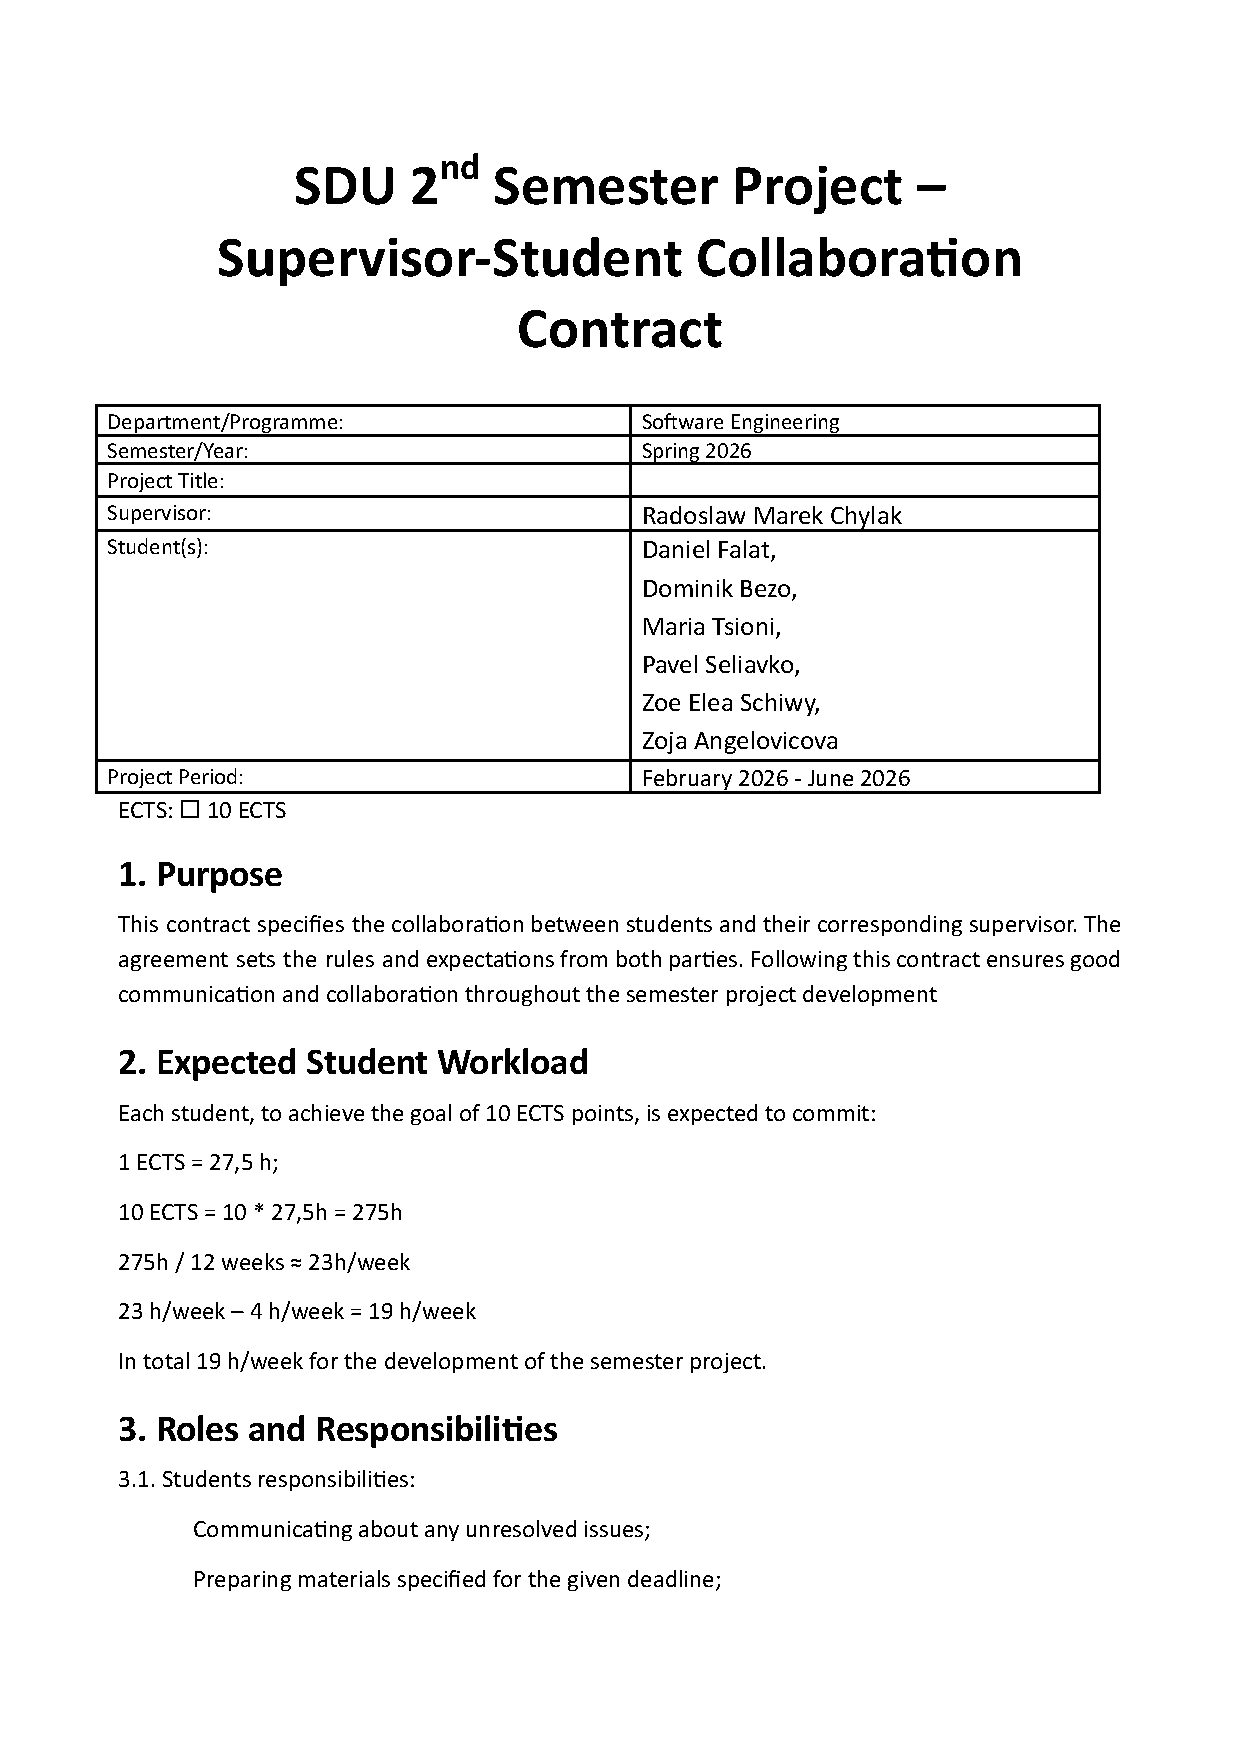
\includepdf[pages=-]{SupervisorAgreement.pdf}
\newpage

Our team agreement contract:
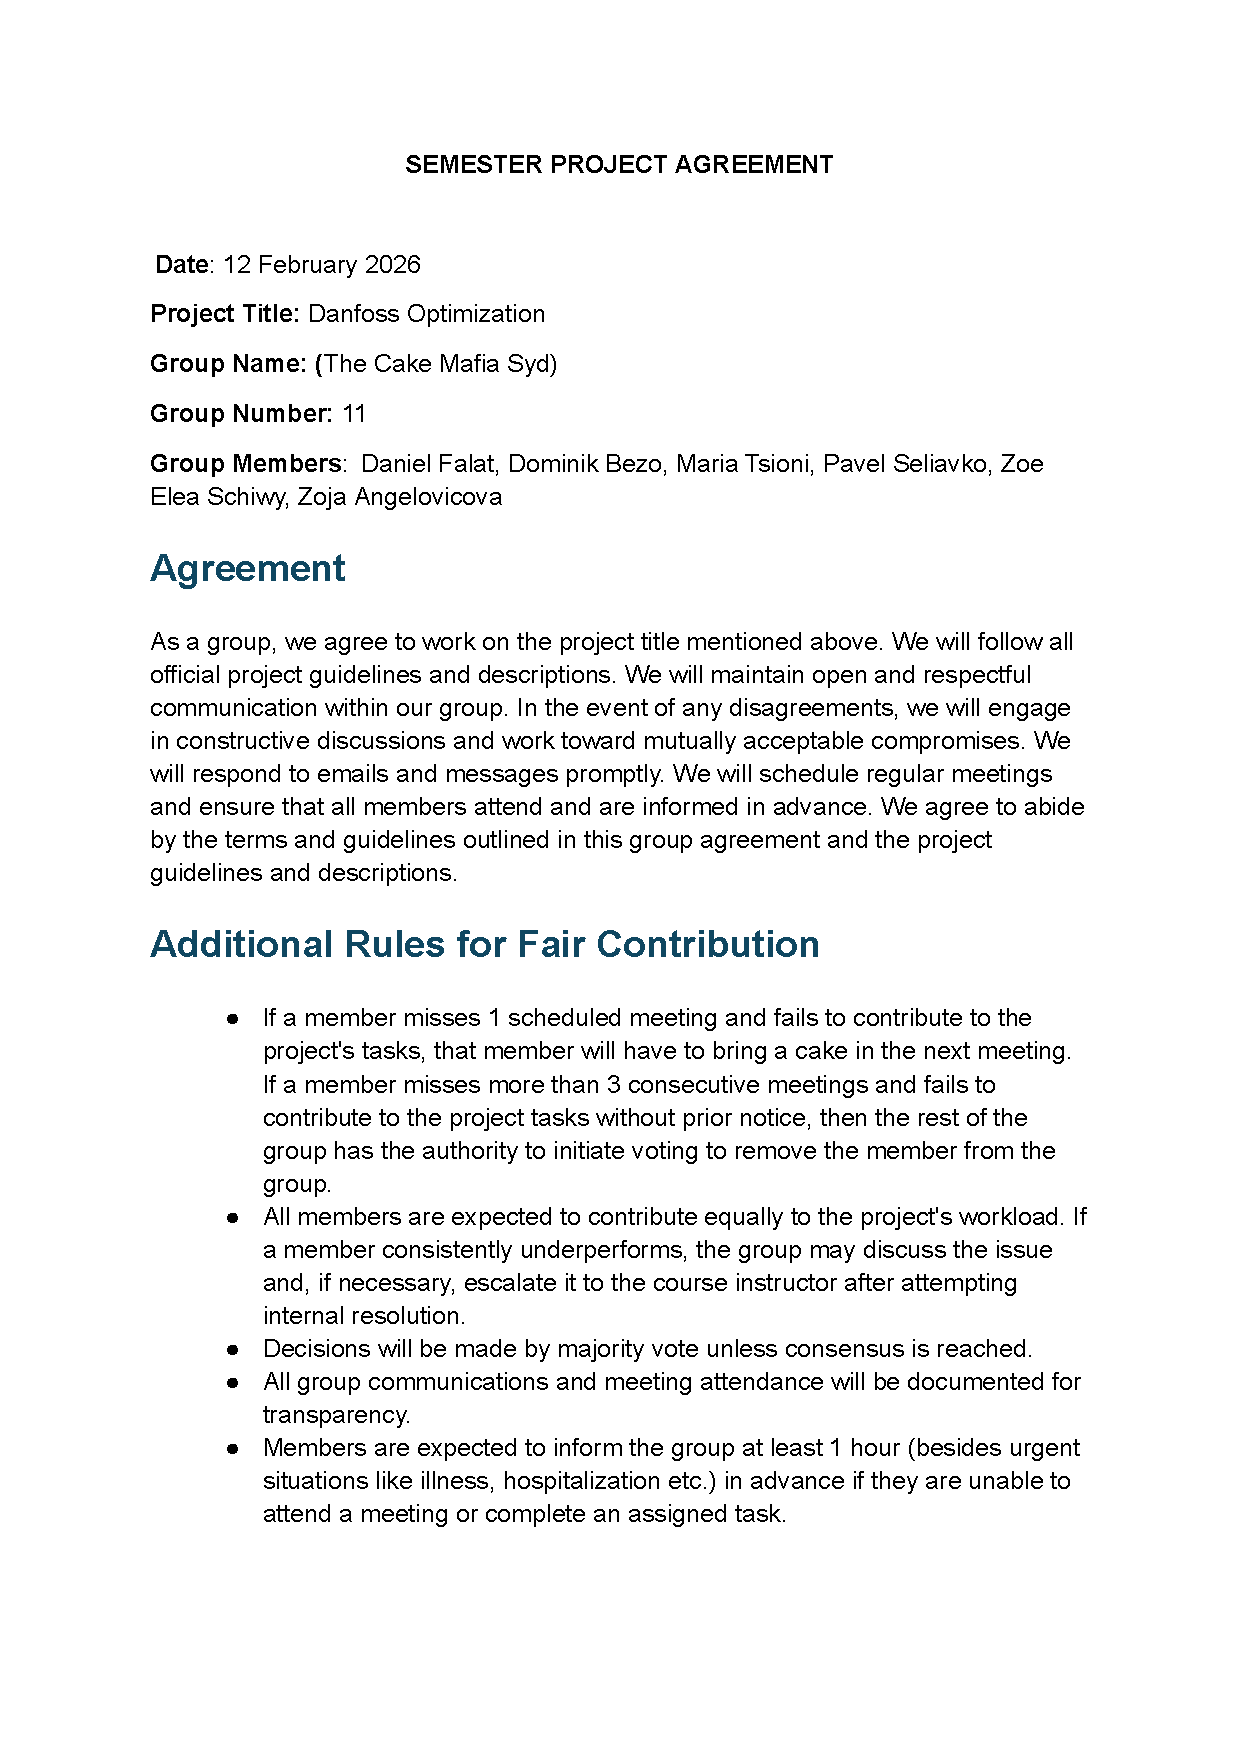
\includepdf[pages=-]{GroupAgreement.pdf}
\newpage

\section{Report Responsibilities Table}
\begin{center}
\begin{tabular}{|p{5cm}|p{5cm}|p{5cm}|} 
\hline
Part & Writer & Reviewer \\ \hline \hline
Abstract & Zoe Elea Schiwy & Dominik Bežo \\ \hline
Introduction & Dominik Bežo & Pavel Seliavko \\ \hline
SCRUM Implementation & Maria Thalia Tsioni & Daniel Falat \\ \hline
Sprints & Zoja Angelovicova & Zoe Elea Schiwy \\ \hline
Solution & Pavel Seliavko & Zoja Angelovicova \\ \hline
Implementation Frontend & Daniel Falat, Dominik Bežo, Zoja Angelovicova & Maria Thalia Tsioni, Pavel Seliavko, Zoe Elea Schiwy \\ \hline
Implementation Backend & Zoe Elea Schiwy & Daniel Falat, Dominik Bežo, Zoja Angelovicova \\ \hline
Implementation Data Management & Maria Thalia Tsioni & Daniel Falat, Dominik Bežo, Zoja Angelovicova \\ \hline
Discussion and Reflection & Daniel Falat & Maria Thalia Tsioni \\ \hline
Conclusion & Zoe Elea Schiwy & Dominik Bežo \\ \hline
References & Maria Thalia Tsioni & Zoja Angelovicova \\ \hline
Acknowledgements & Daniel Falat & Maria Thalia Tsioni \\ \hline
Appendix & Pavel Seliavko & Maria Thalia Tsioni \\ \hline
\end{tabular}
\end{center}
\newpage

\section{Meeting Logs}
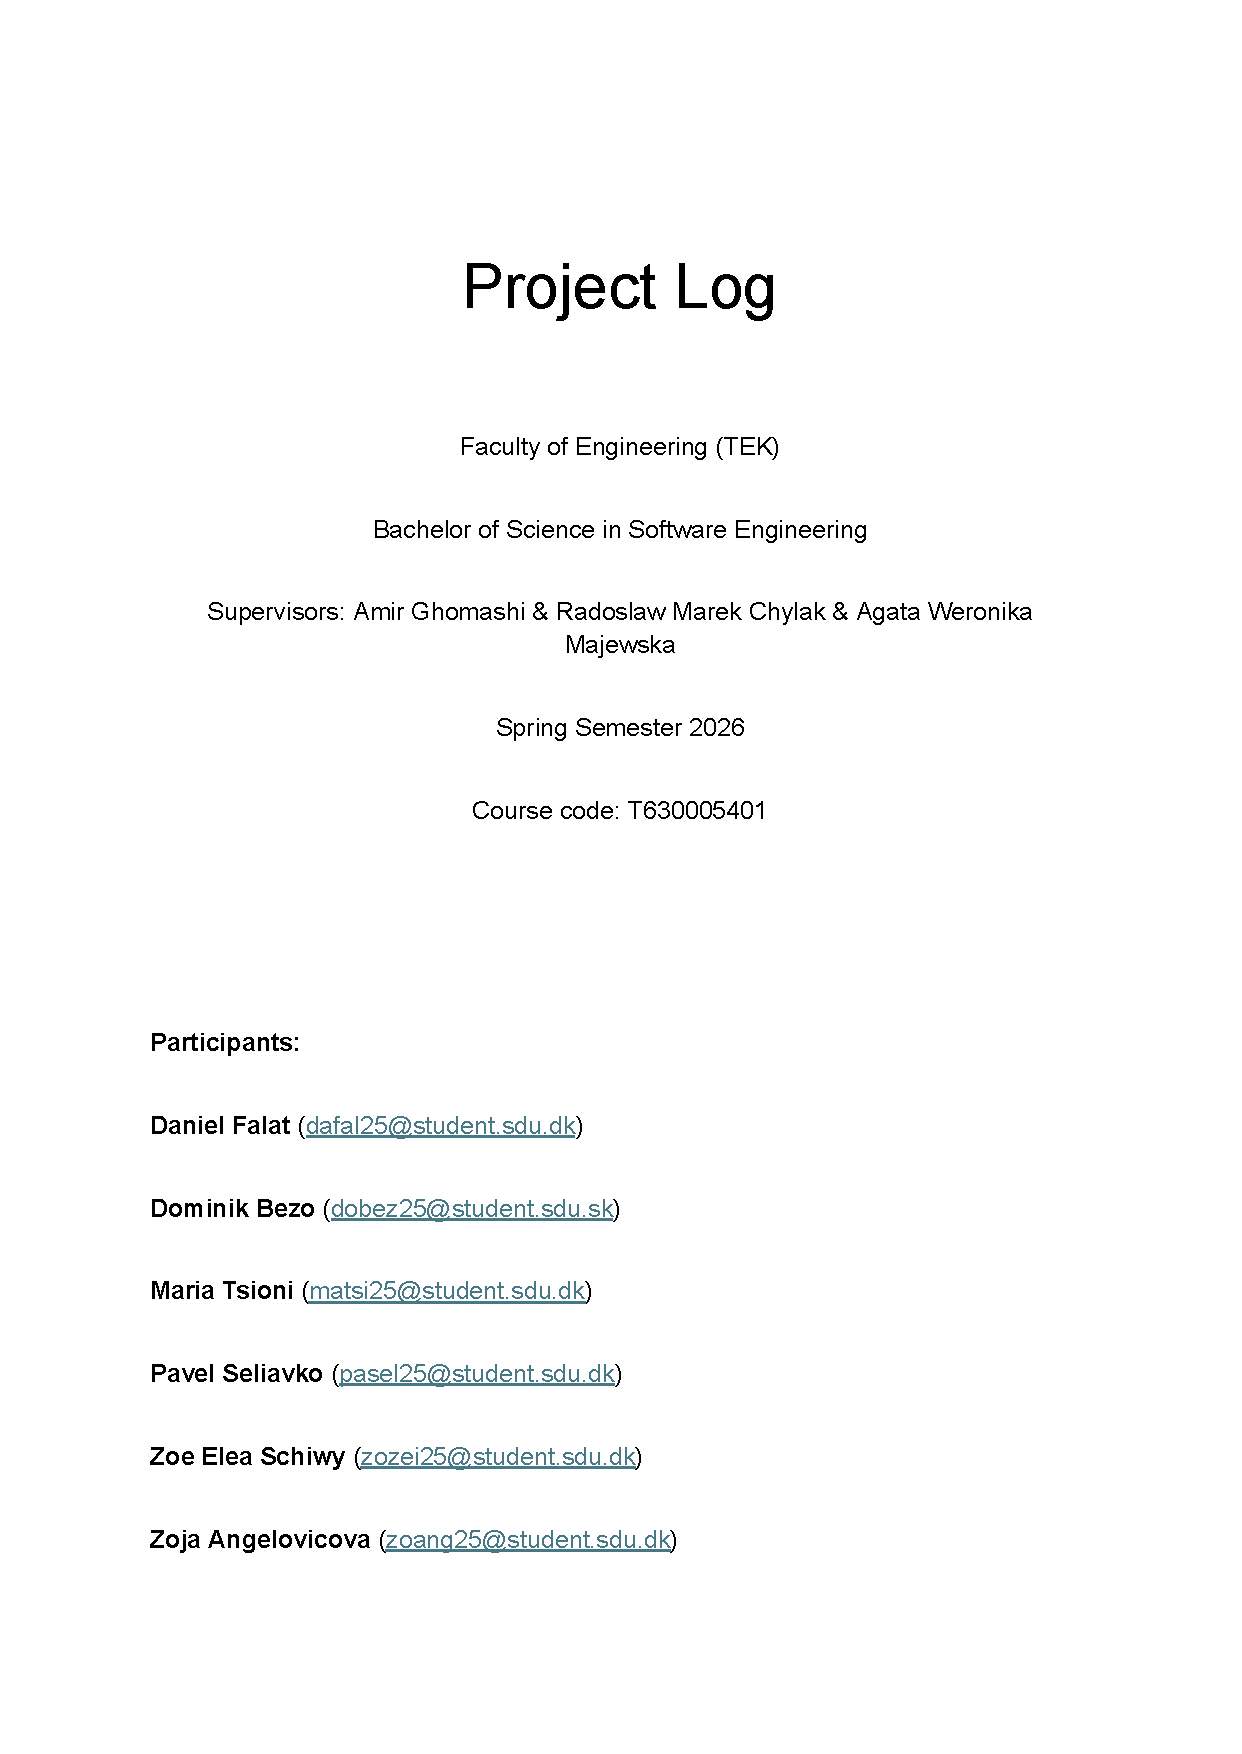
\includepdf[pages=-]{MeetingLogs.pdf}
\newpage

\section{Product Increments}
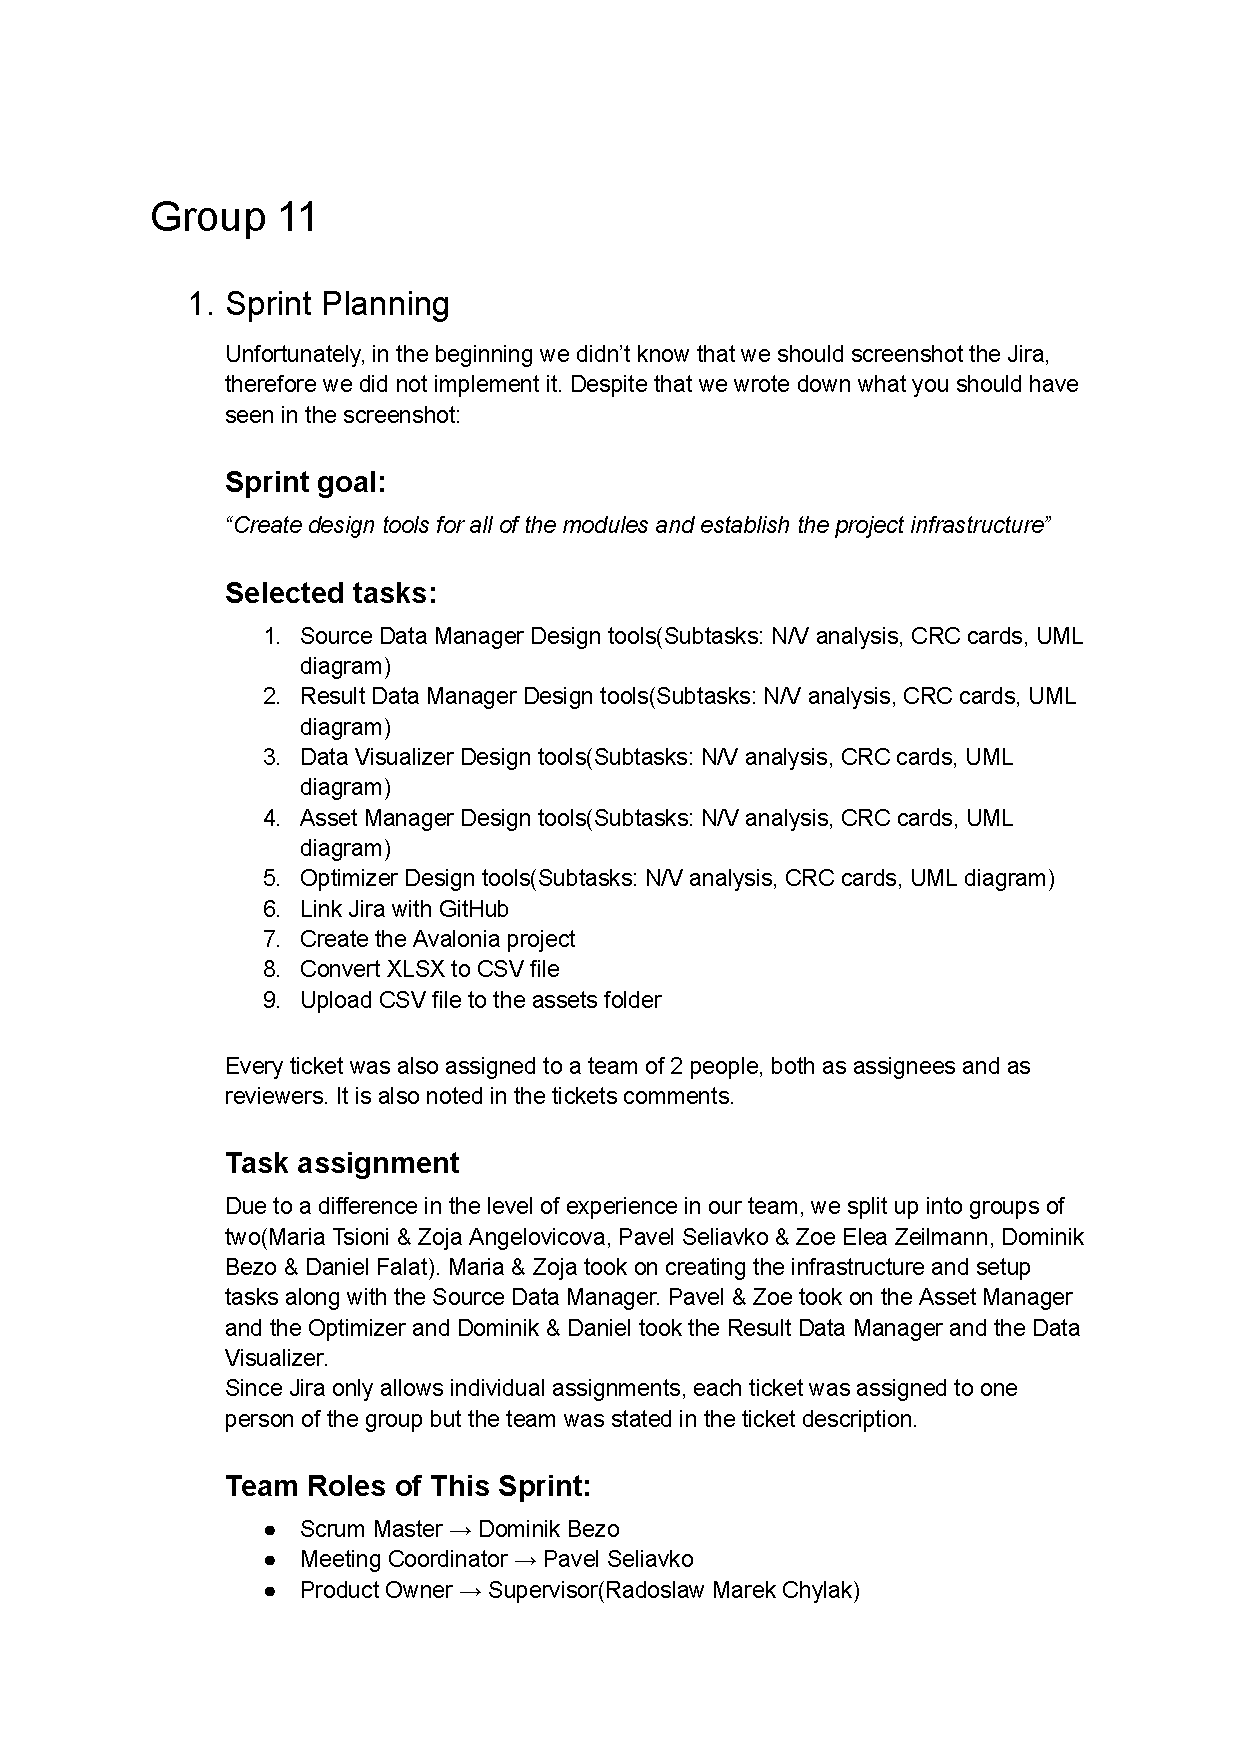
\includepdf[pages=-]{PI1.pdf}
\newpage
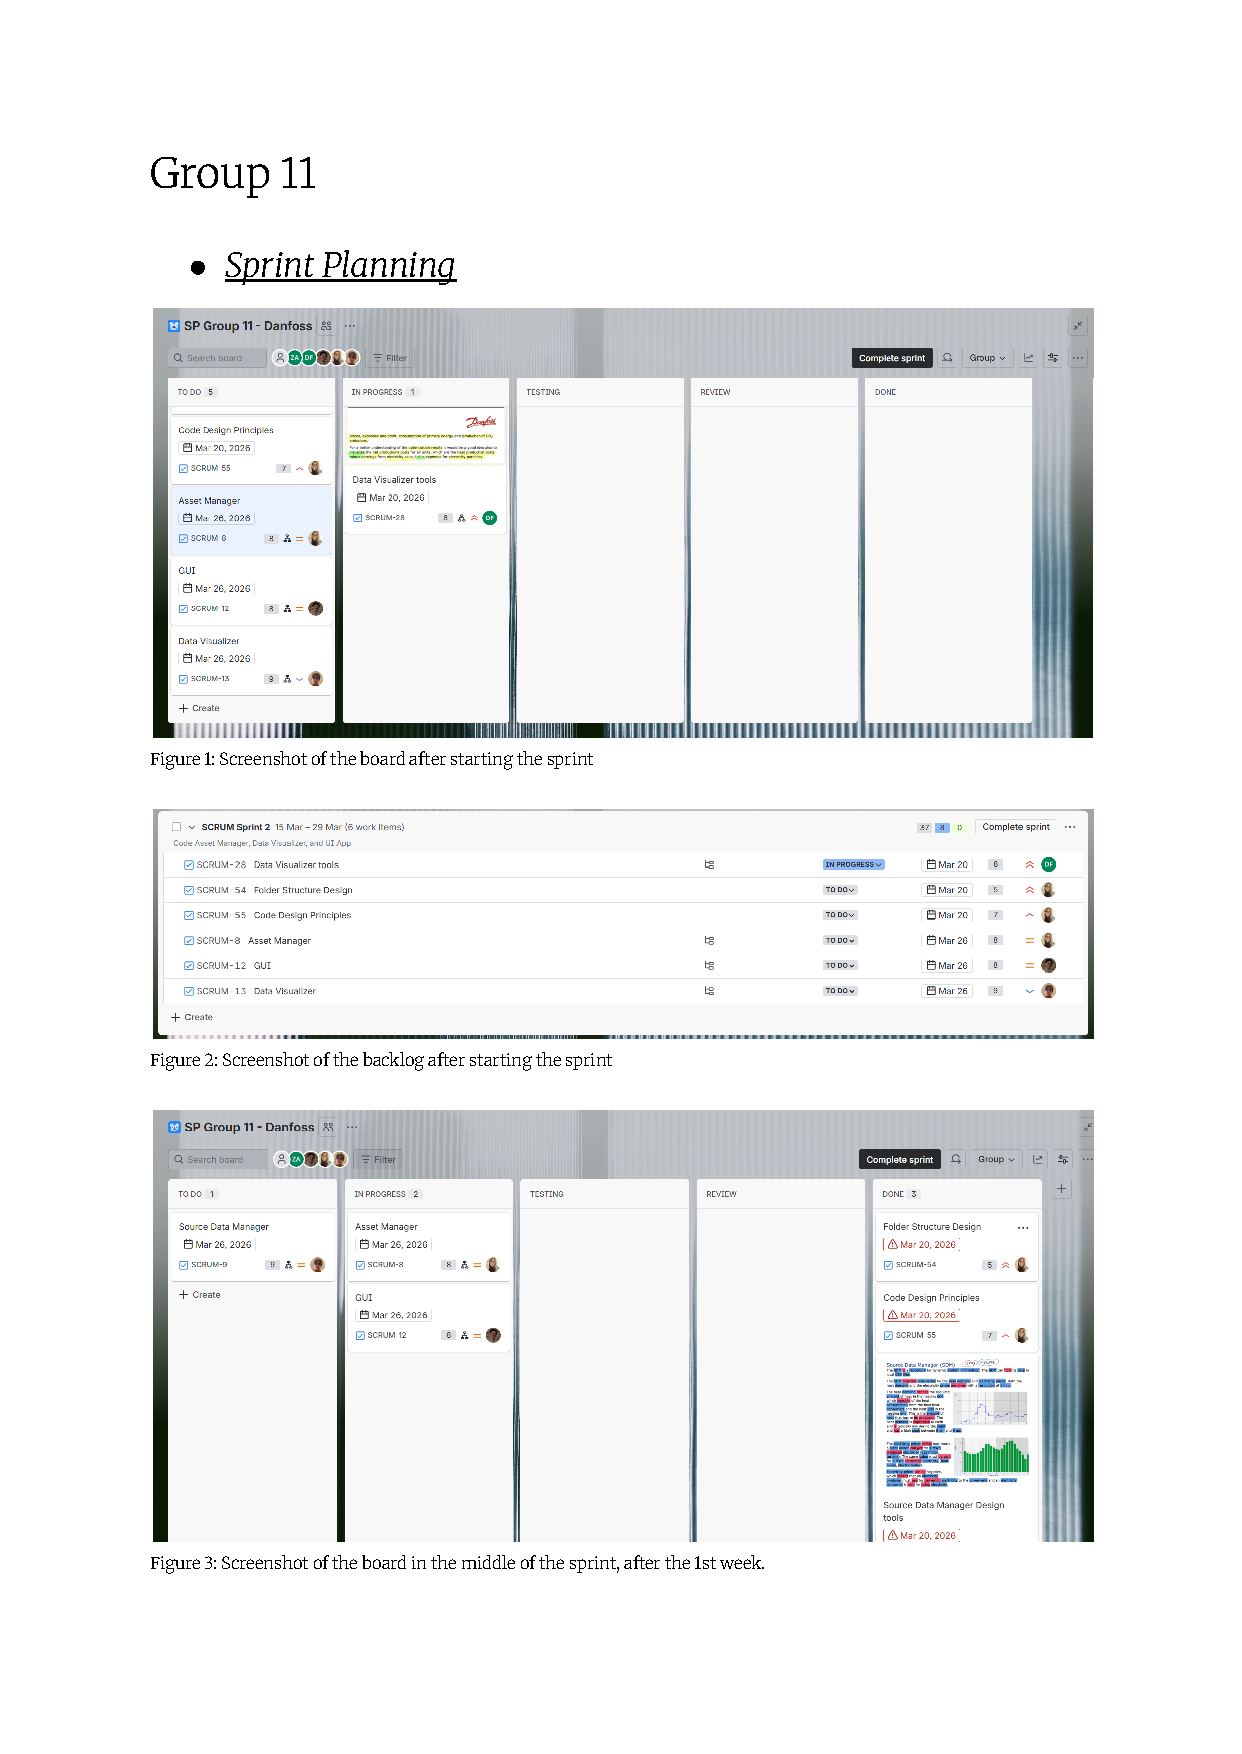
\includepdf[pages=-]{PI2.pdf}
\newpage
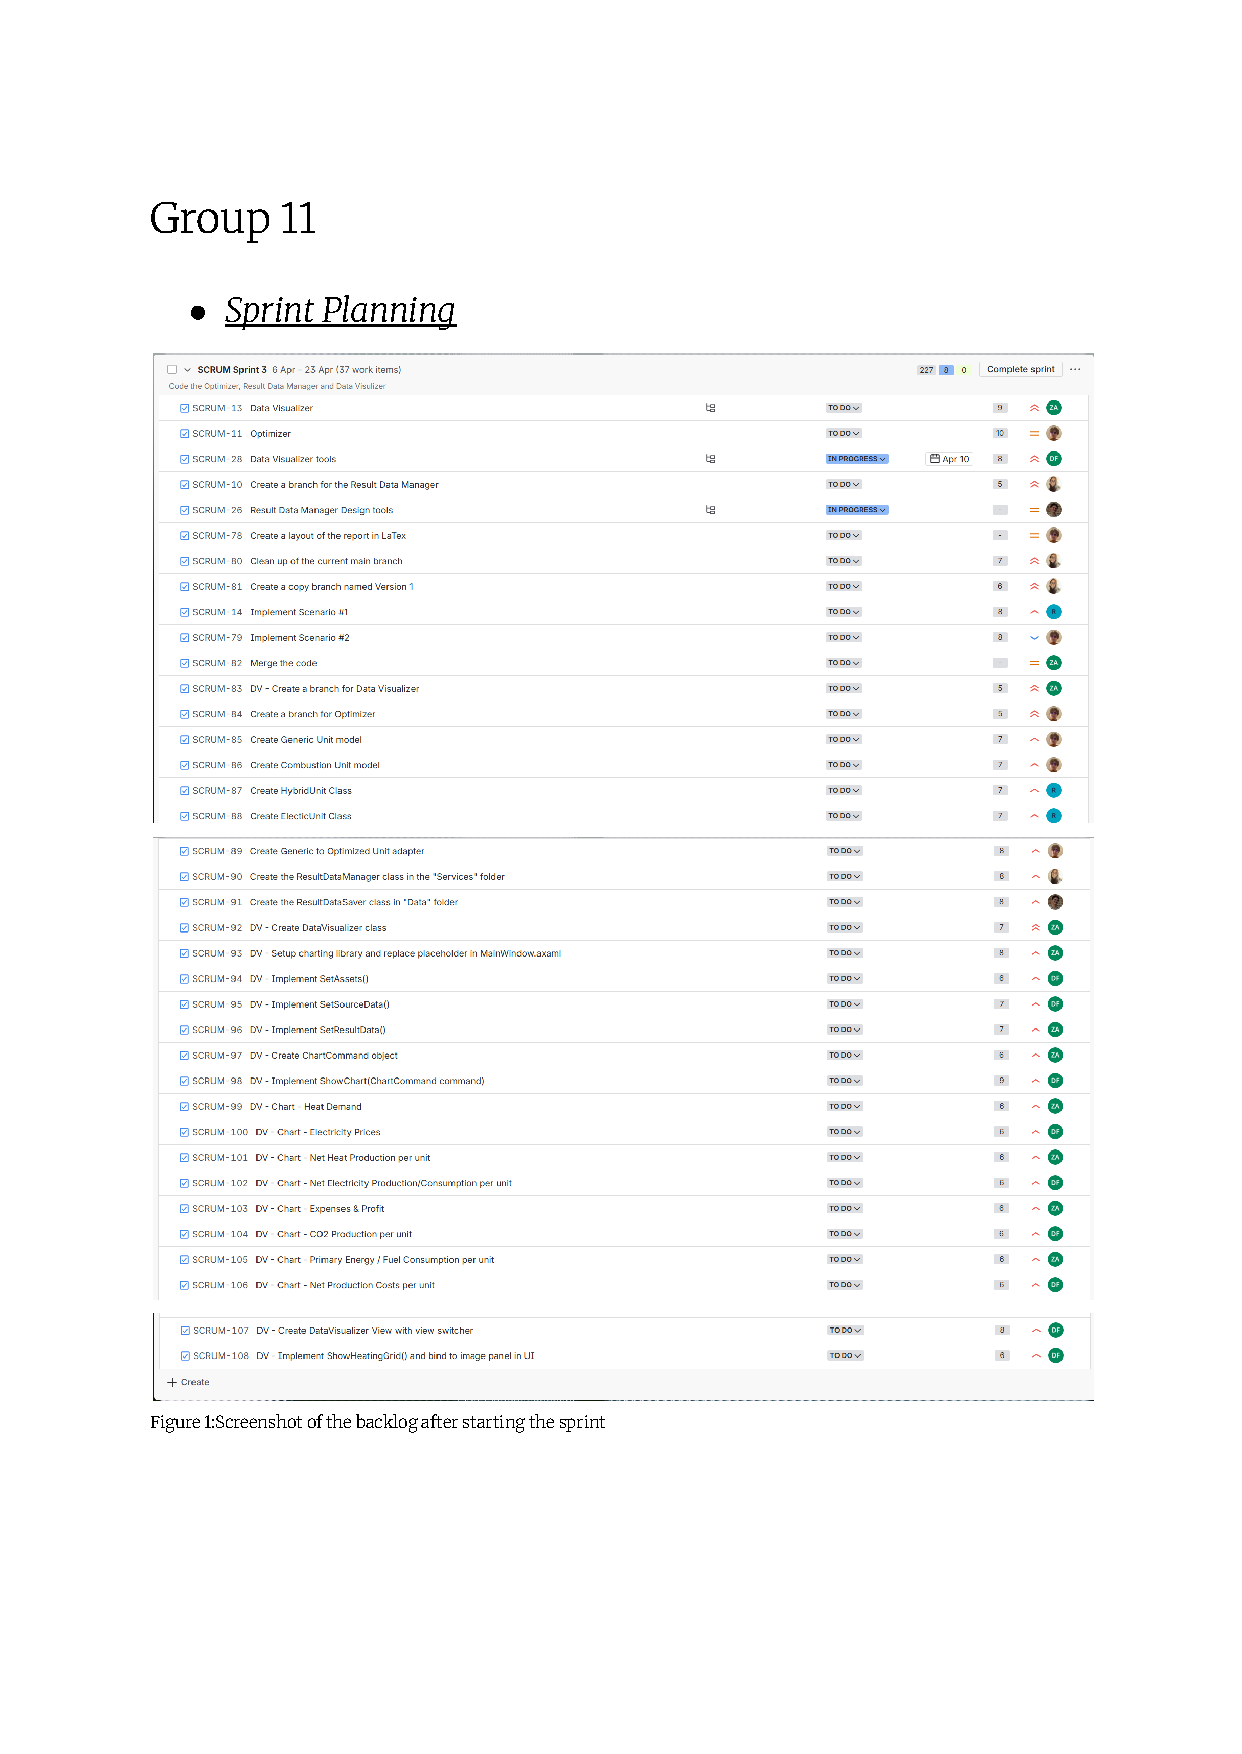
\includepdf[pages=-]{PI3.pdf}
\newpage
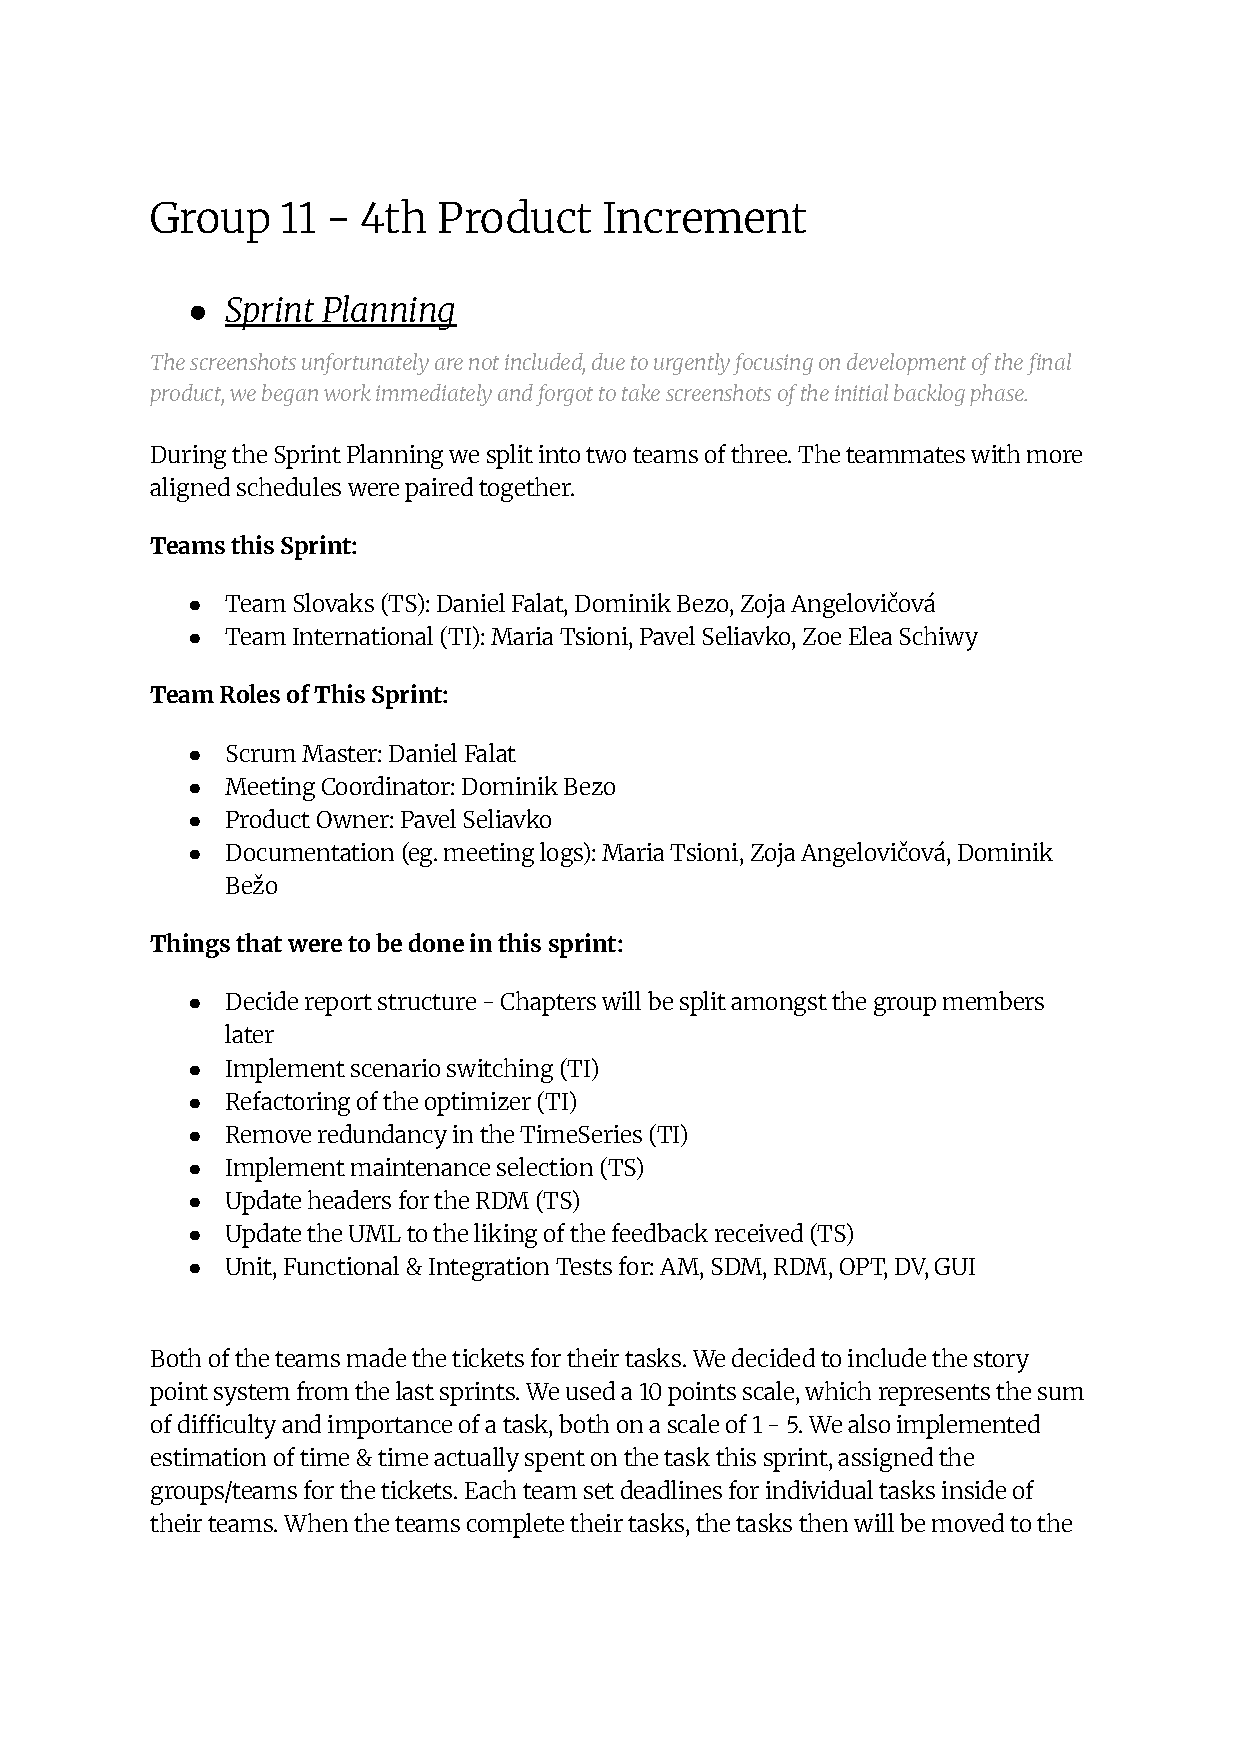
\includepdf[pages=-]{PI4.pdf}
\newpage
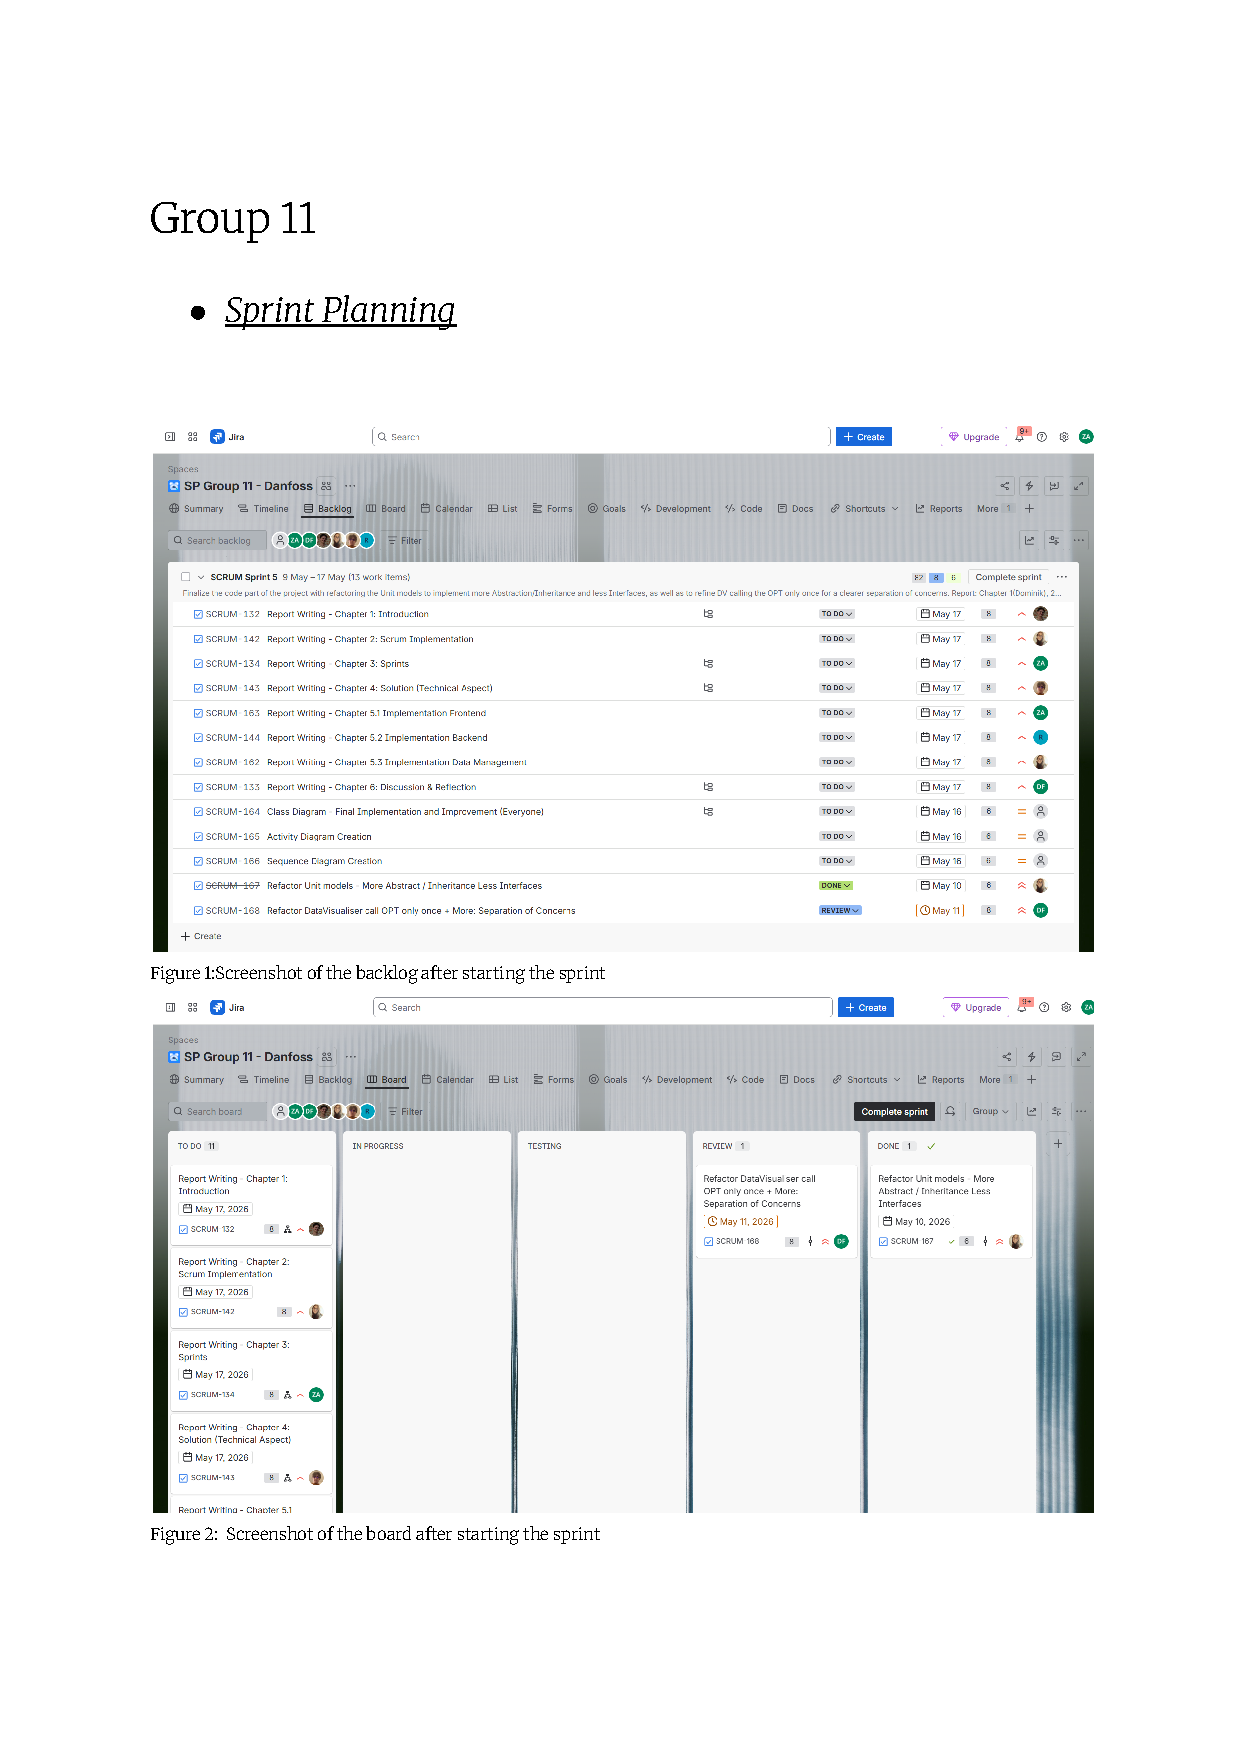
\includepdf[pages=-]{PI5.pdf}
\newpage

\section{Other UML Diagrams}
Component Diagram:
\begin{figure}[h]
    \centering
    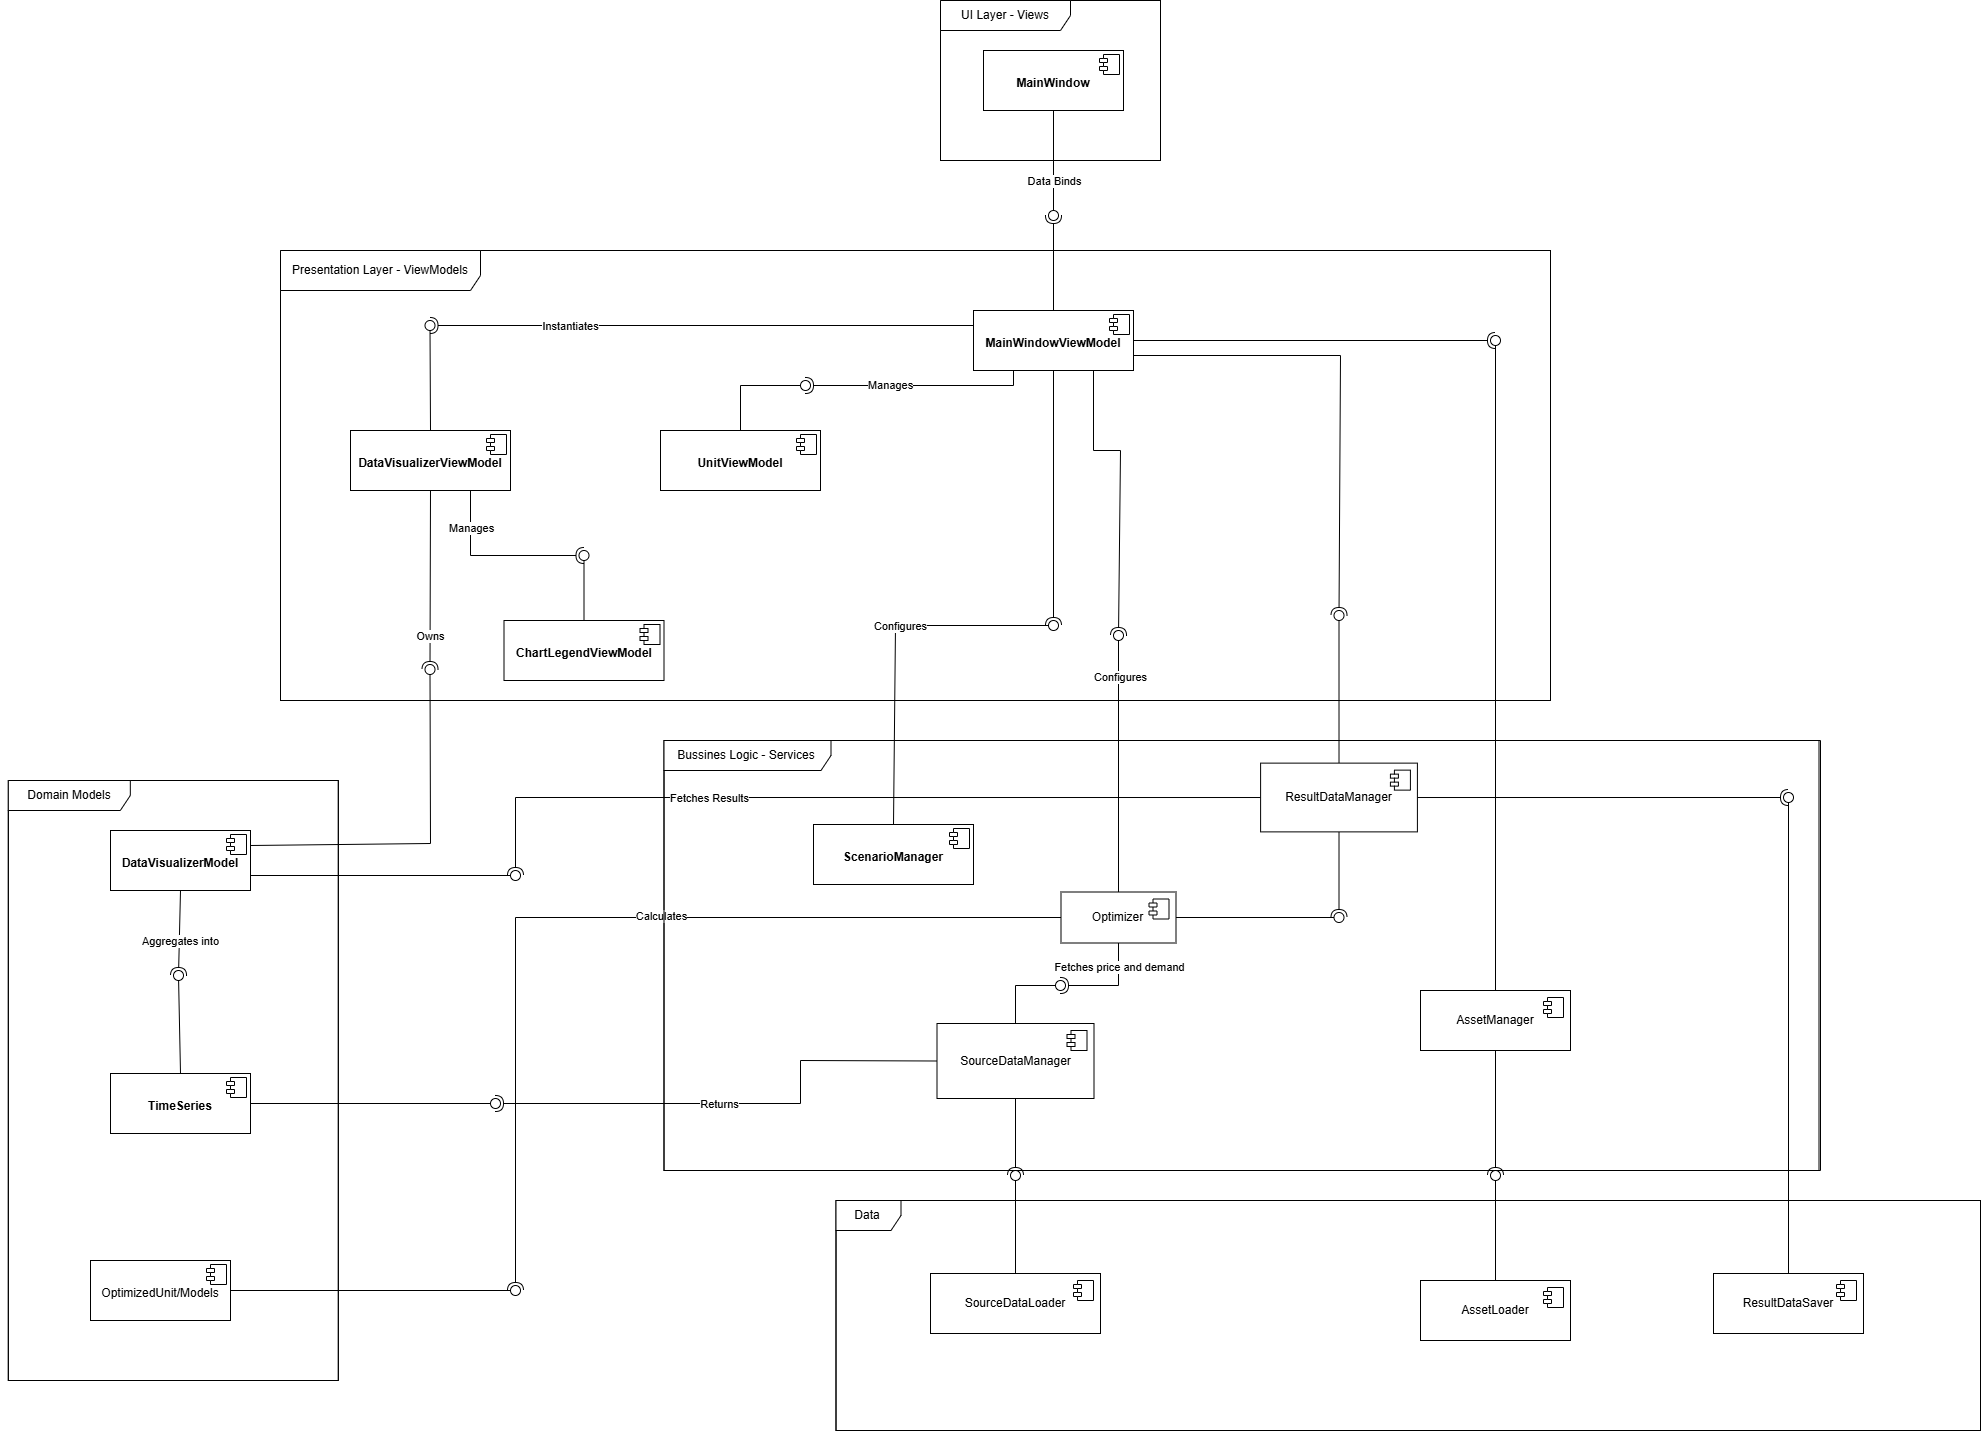
\includegraphics[width=1\textwidth]{ComponentDiagram.png}
    \label{fig:ComponentDiagram}
\end{figure}
\newpage

Use Case Diagram:
\begin{figure}[h]
    \centering
    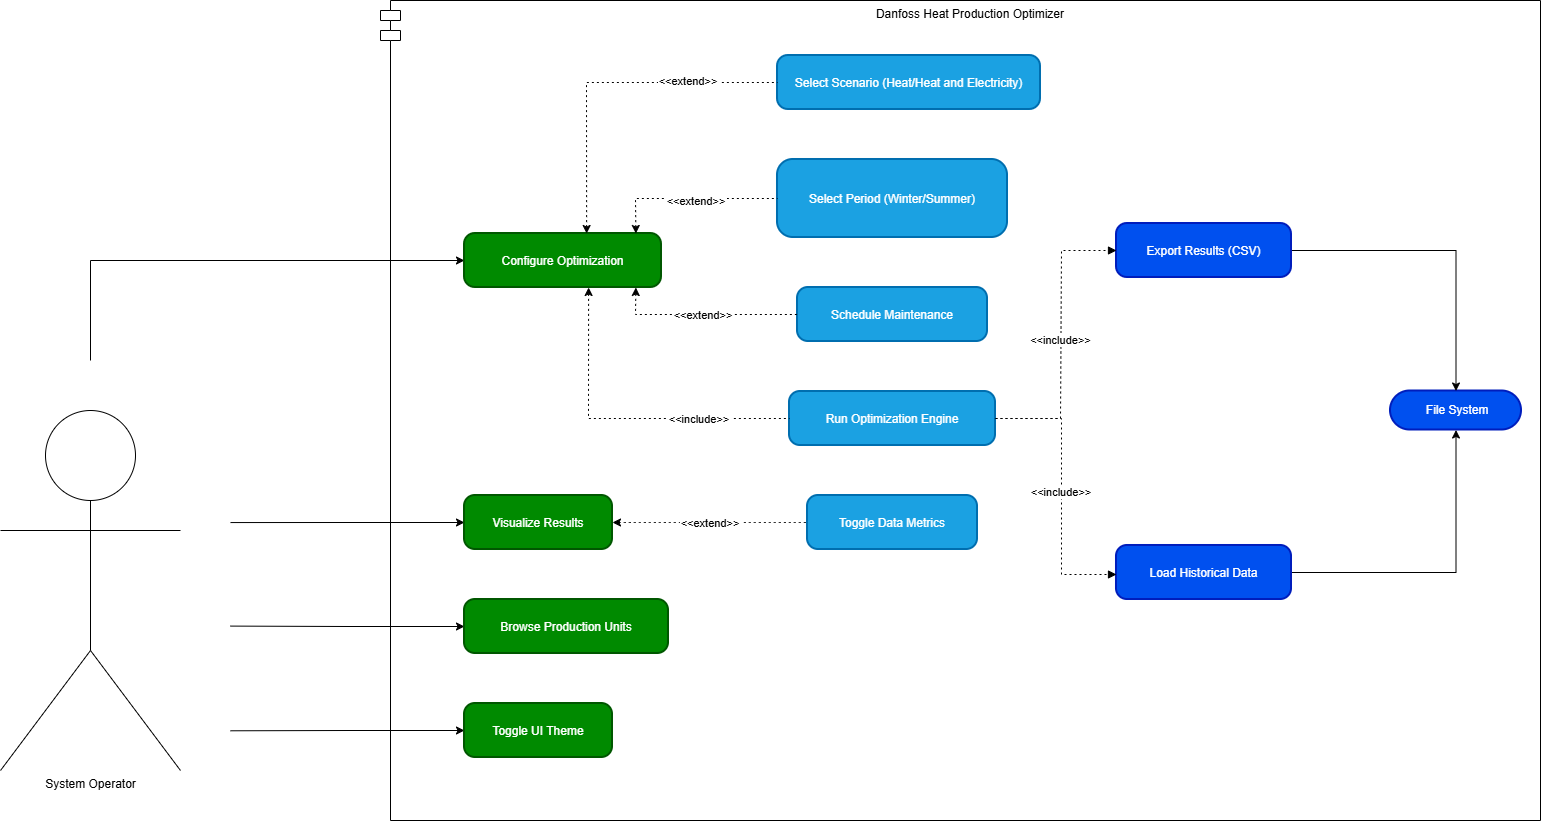
\includegraphics[width=1\textwidth]{UseCaseDiagram.png}
    \label{fig:UseCaseDiagram}
\end{figure}
\newpage

\section{Figma Prototype}
Figma prototype can be found \href{https://www.figma.com/proto/i0pHM1HkLseAXNr38pAF1n/HeatOn-Optimization-Mock-up?node-id=128-1104&t=enIEEG0X7Ny772fb-1}{here}

\section{Early Sketches}
Daniel's Sketch:
\begin{figure}[h]
    \centering
    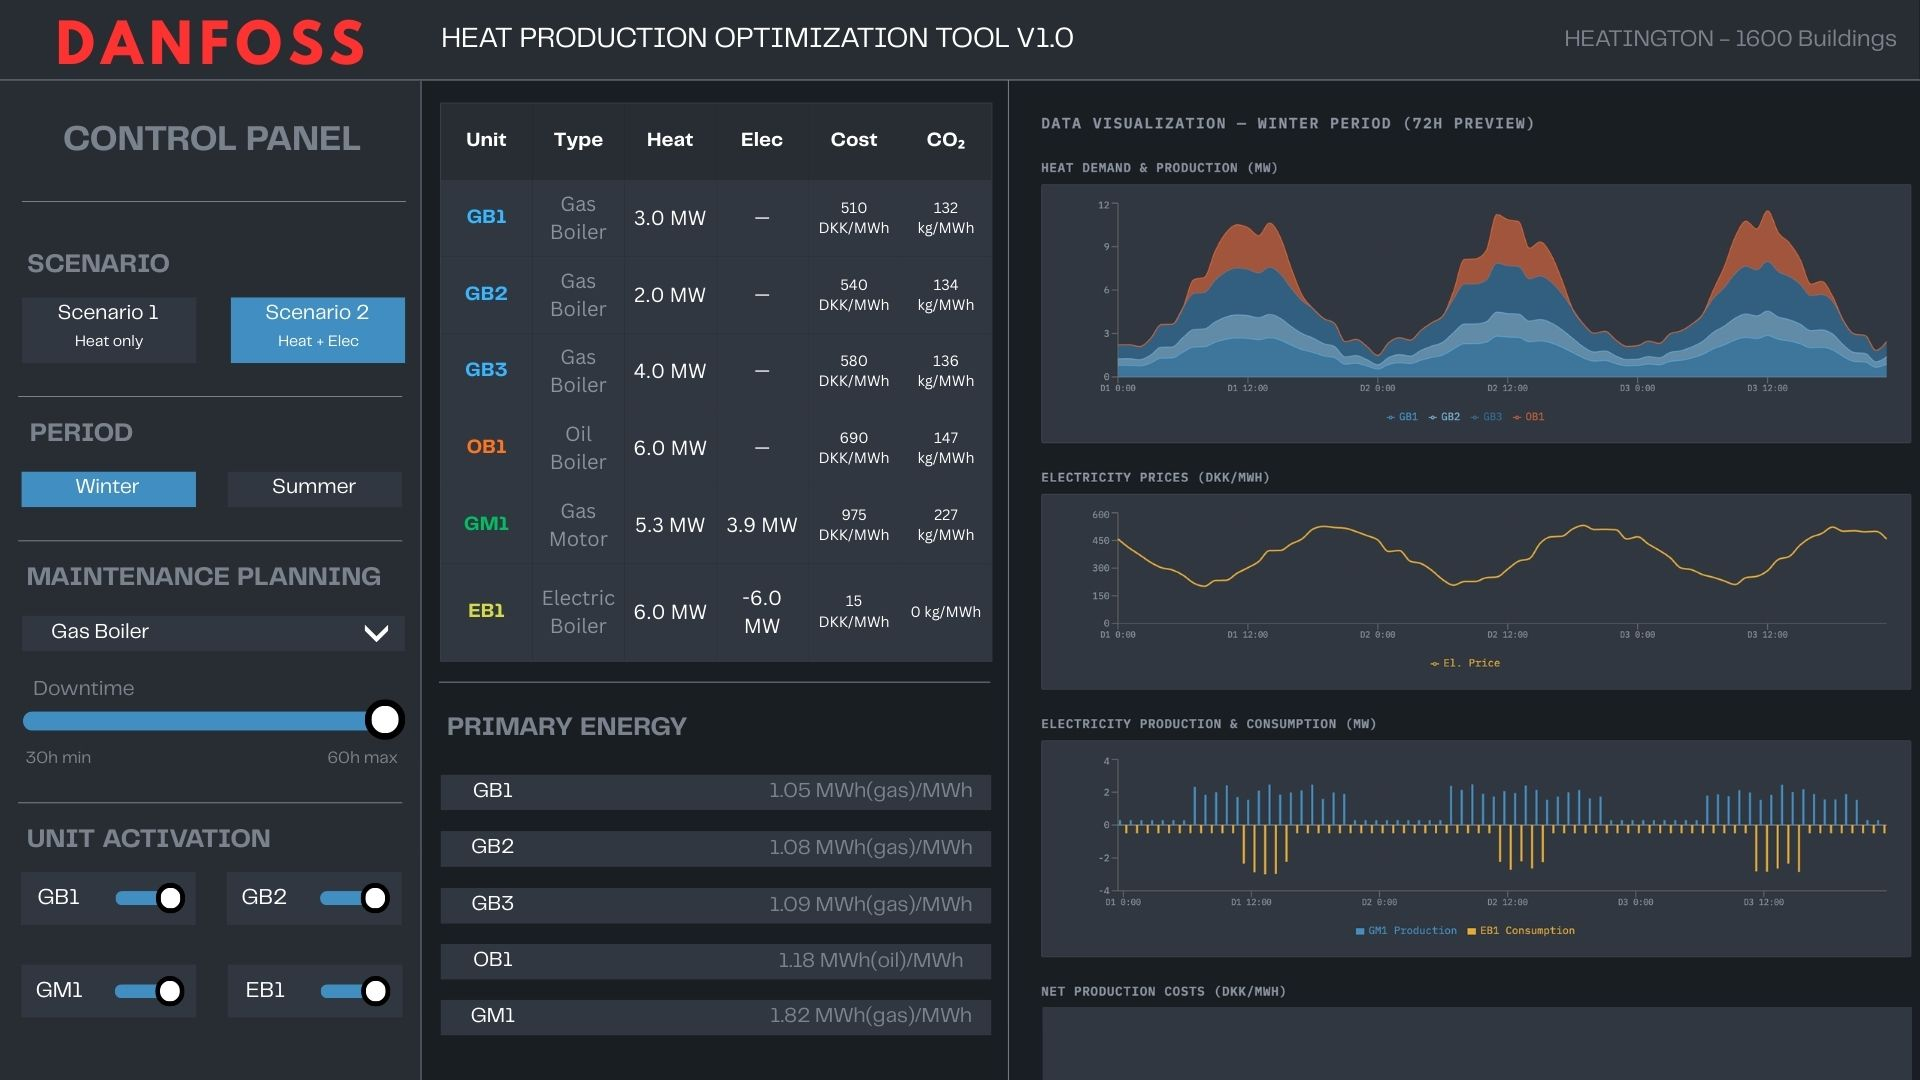
\includegraphics[width=1\textwidth]{DanielSketch.jpg}
    \label{fig:DanielSketch}
\end{figure}
\newpage

Dominik's Sketch:
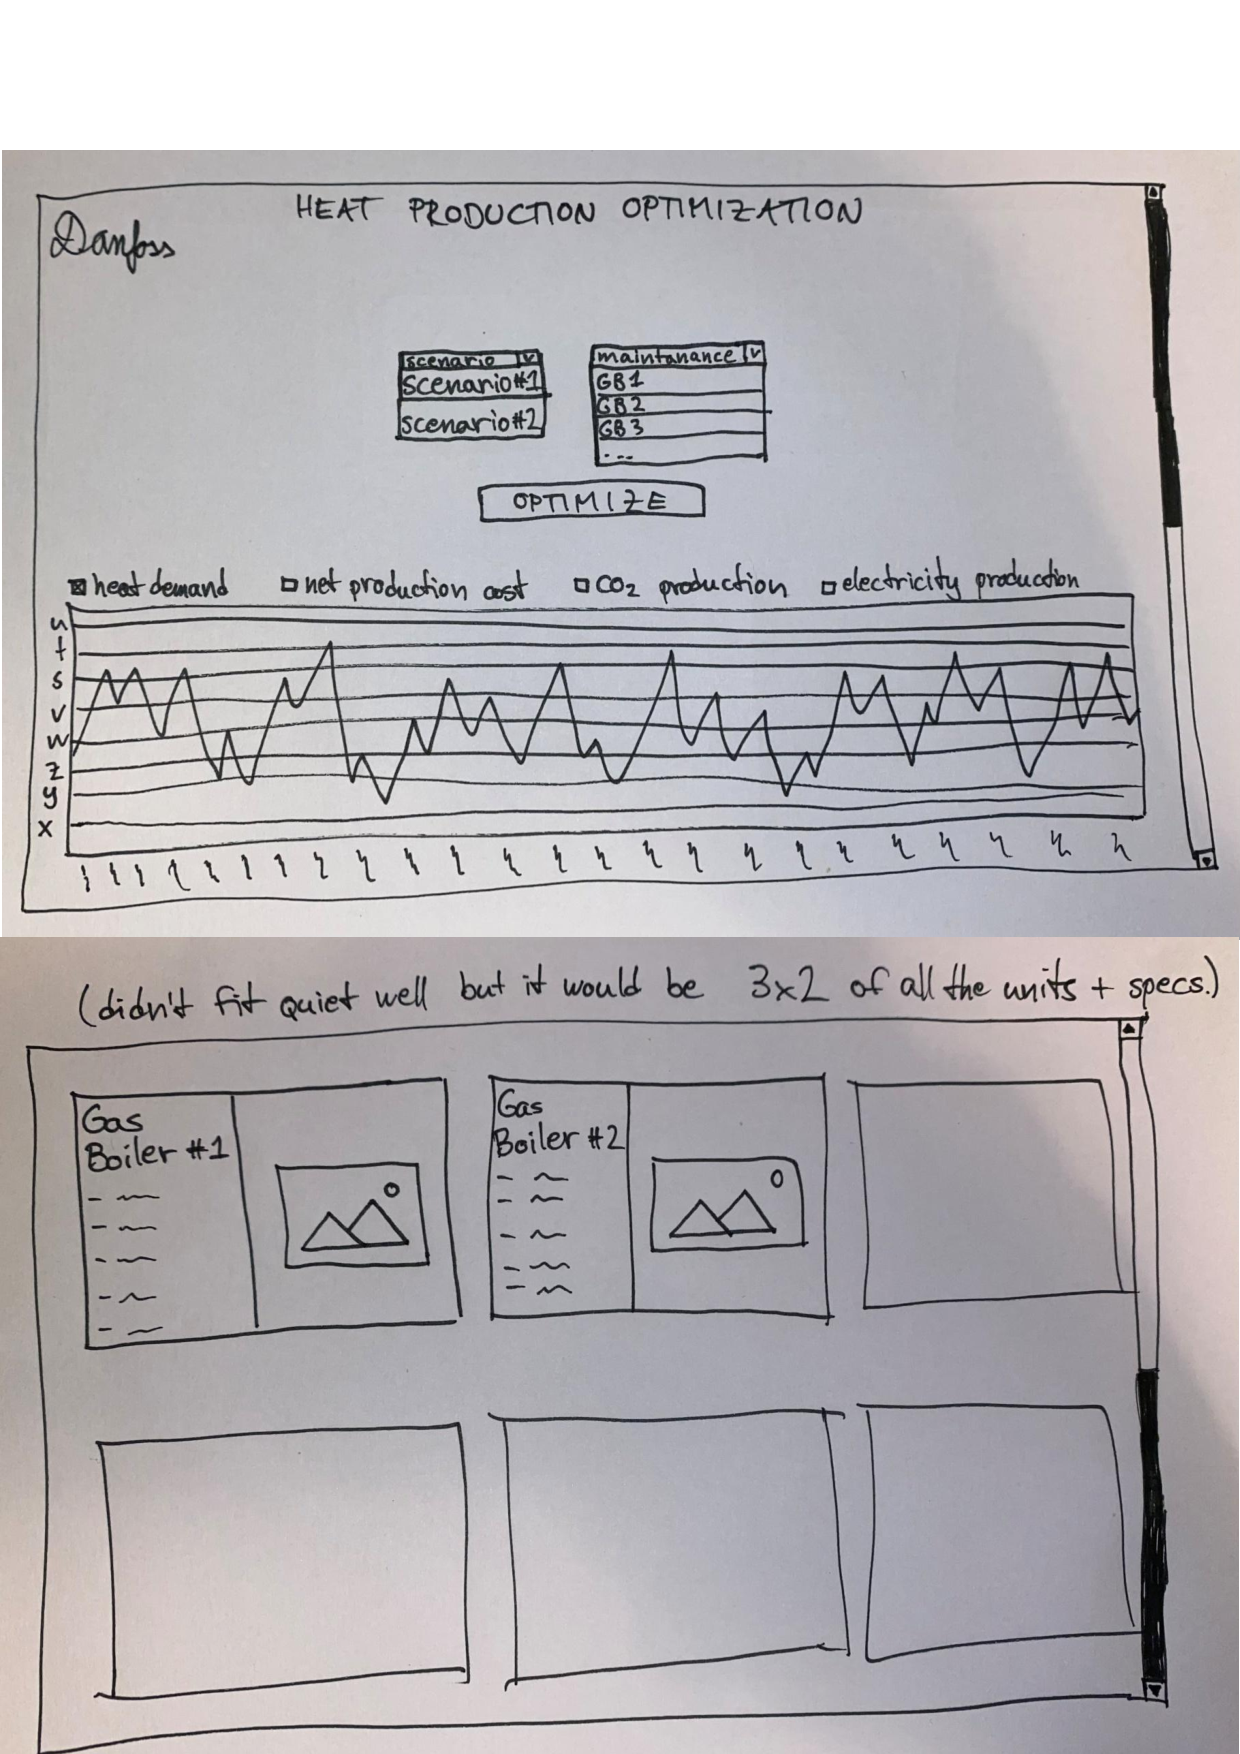
\includepdf[pages=-]{DominikSketch.pdf}
\newpage

Maria's Sketch:
\begin{figure}[h]
    \centering
    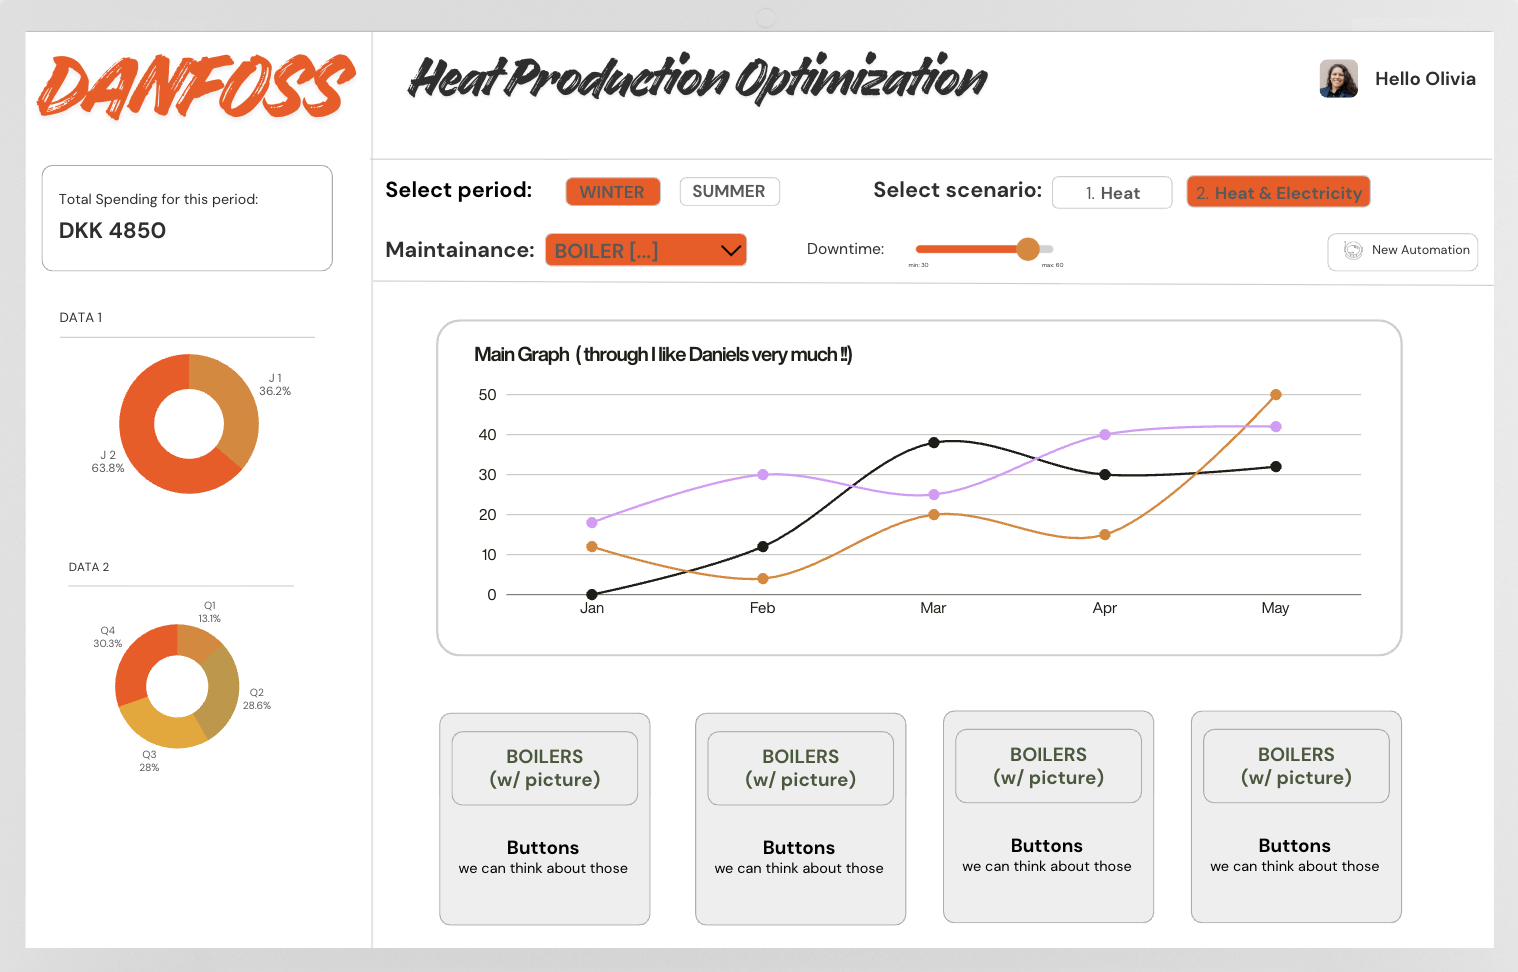
\includegraphics[width=1\textwidth]{MariaSketch.png}
    \label{fig:MariaSketch}
\end{figure}
\newpage

Pavel's Sketch:
\begin{figure}[h]
    \centering
    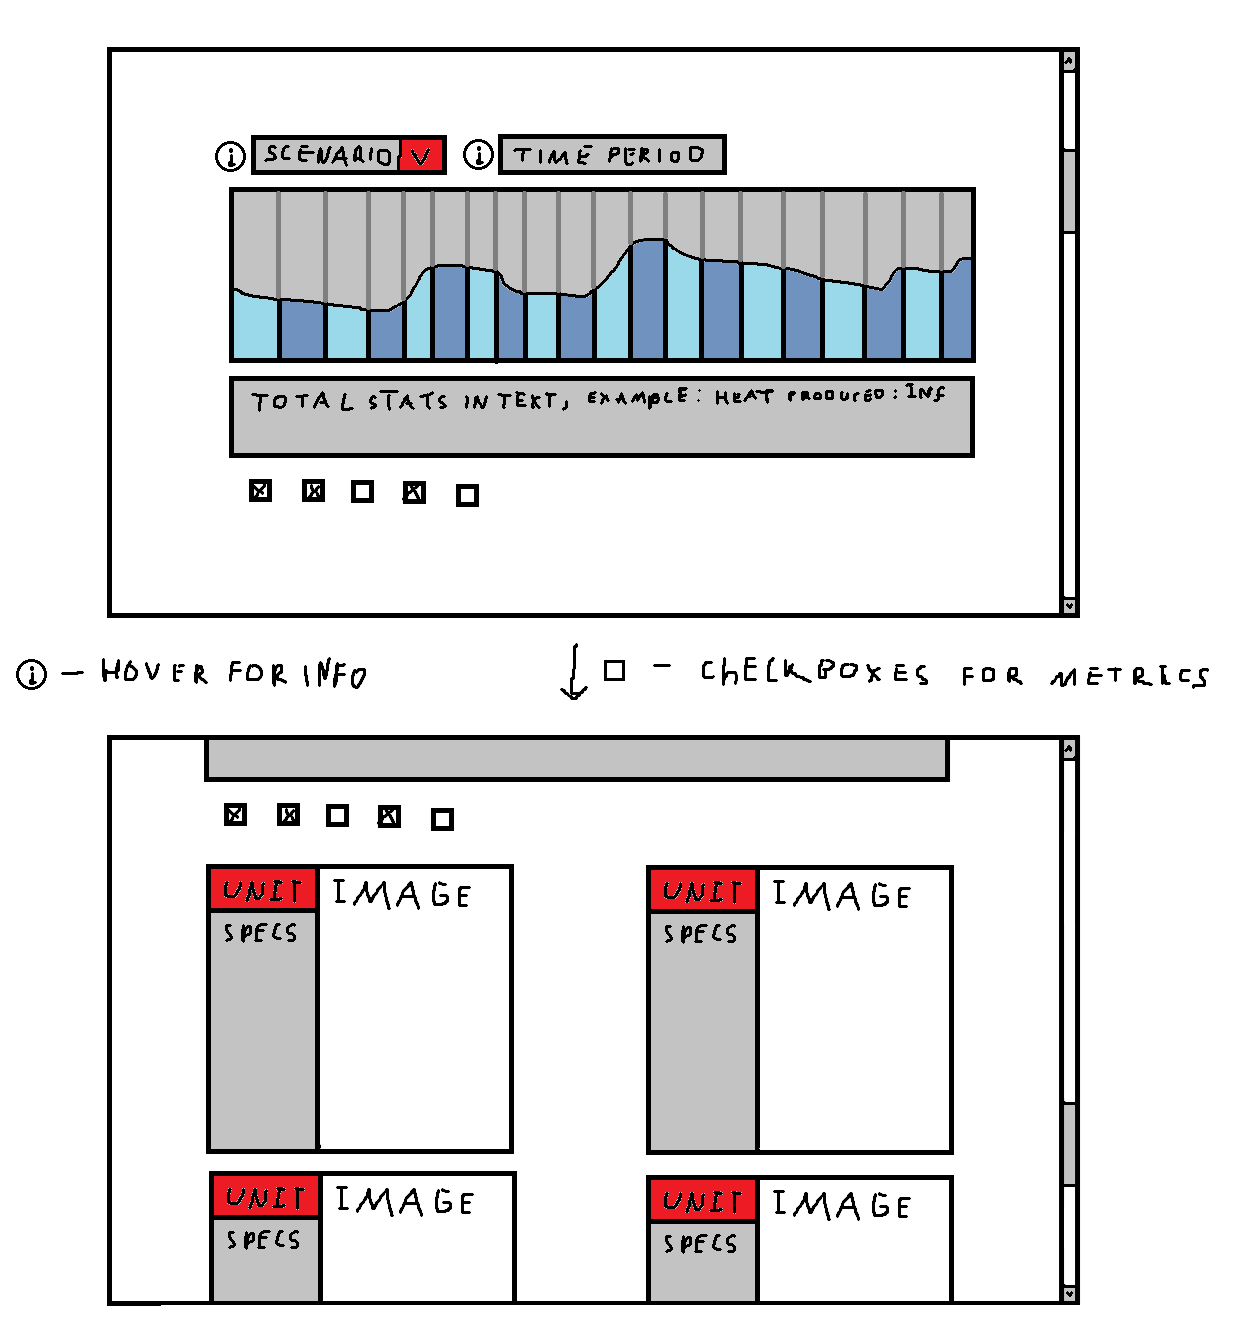
\includegraphics[width=1\textwidth]{PavelSketch.png}
    \label{fig:PavelSketch}
\end{figure}
\newpage

Zoja's Sketches:
\begin{figure}[h]
    \centering
    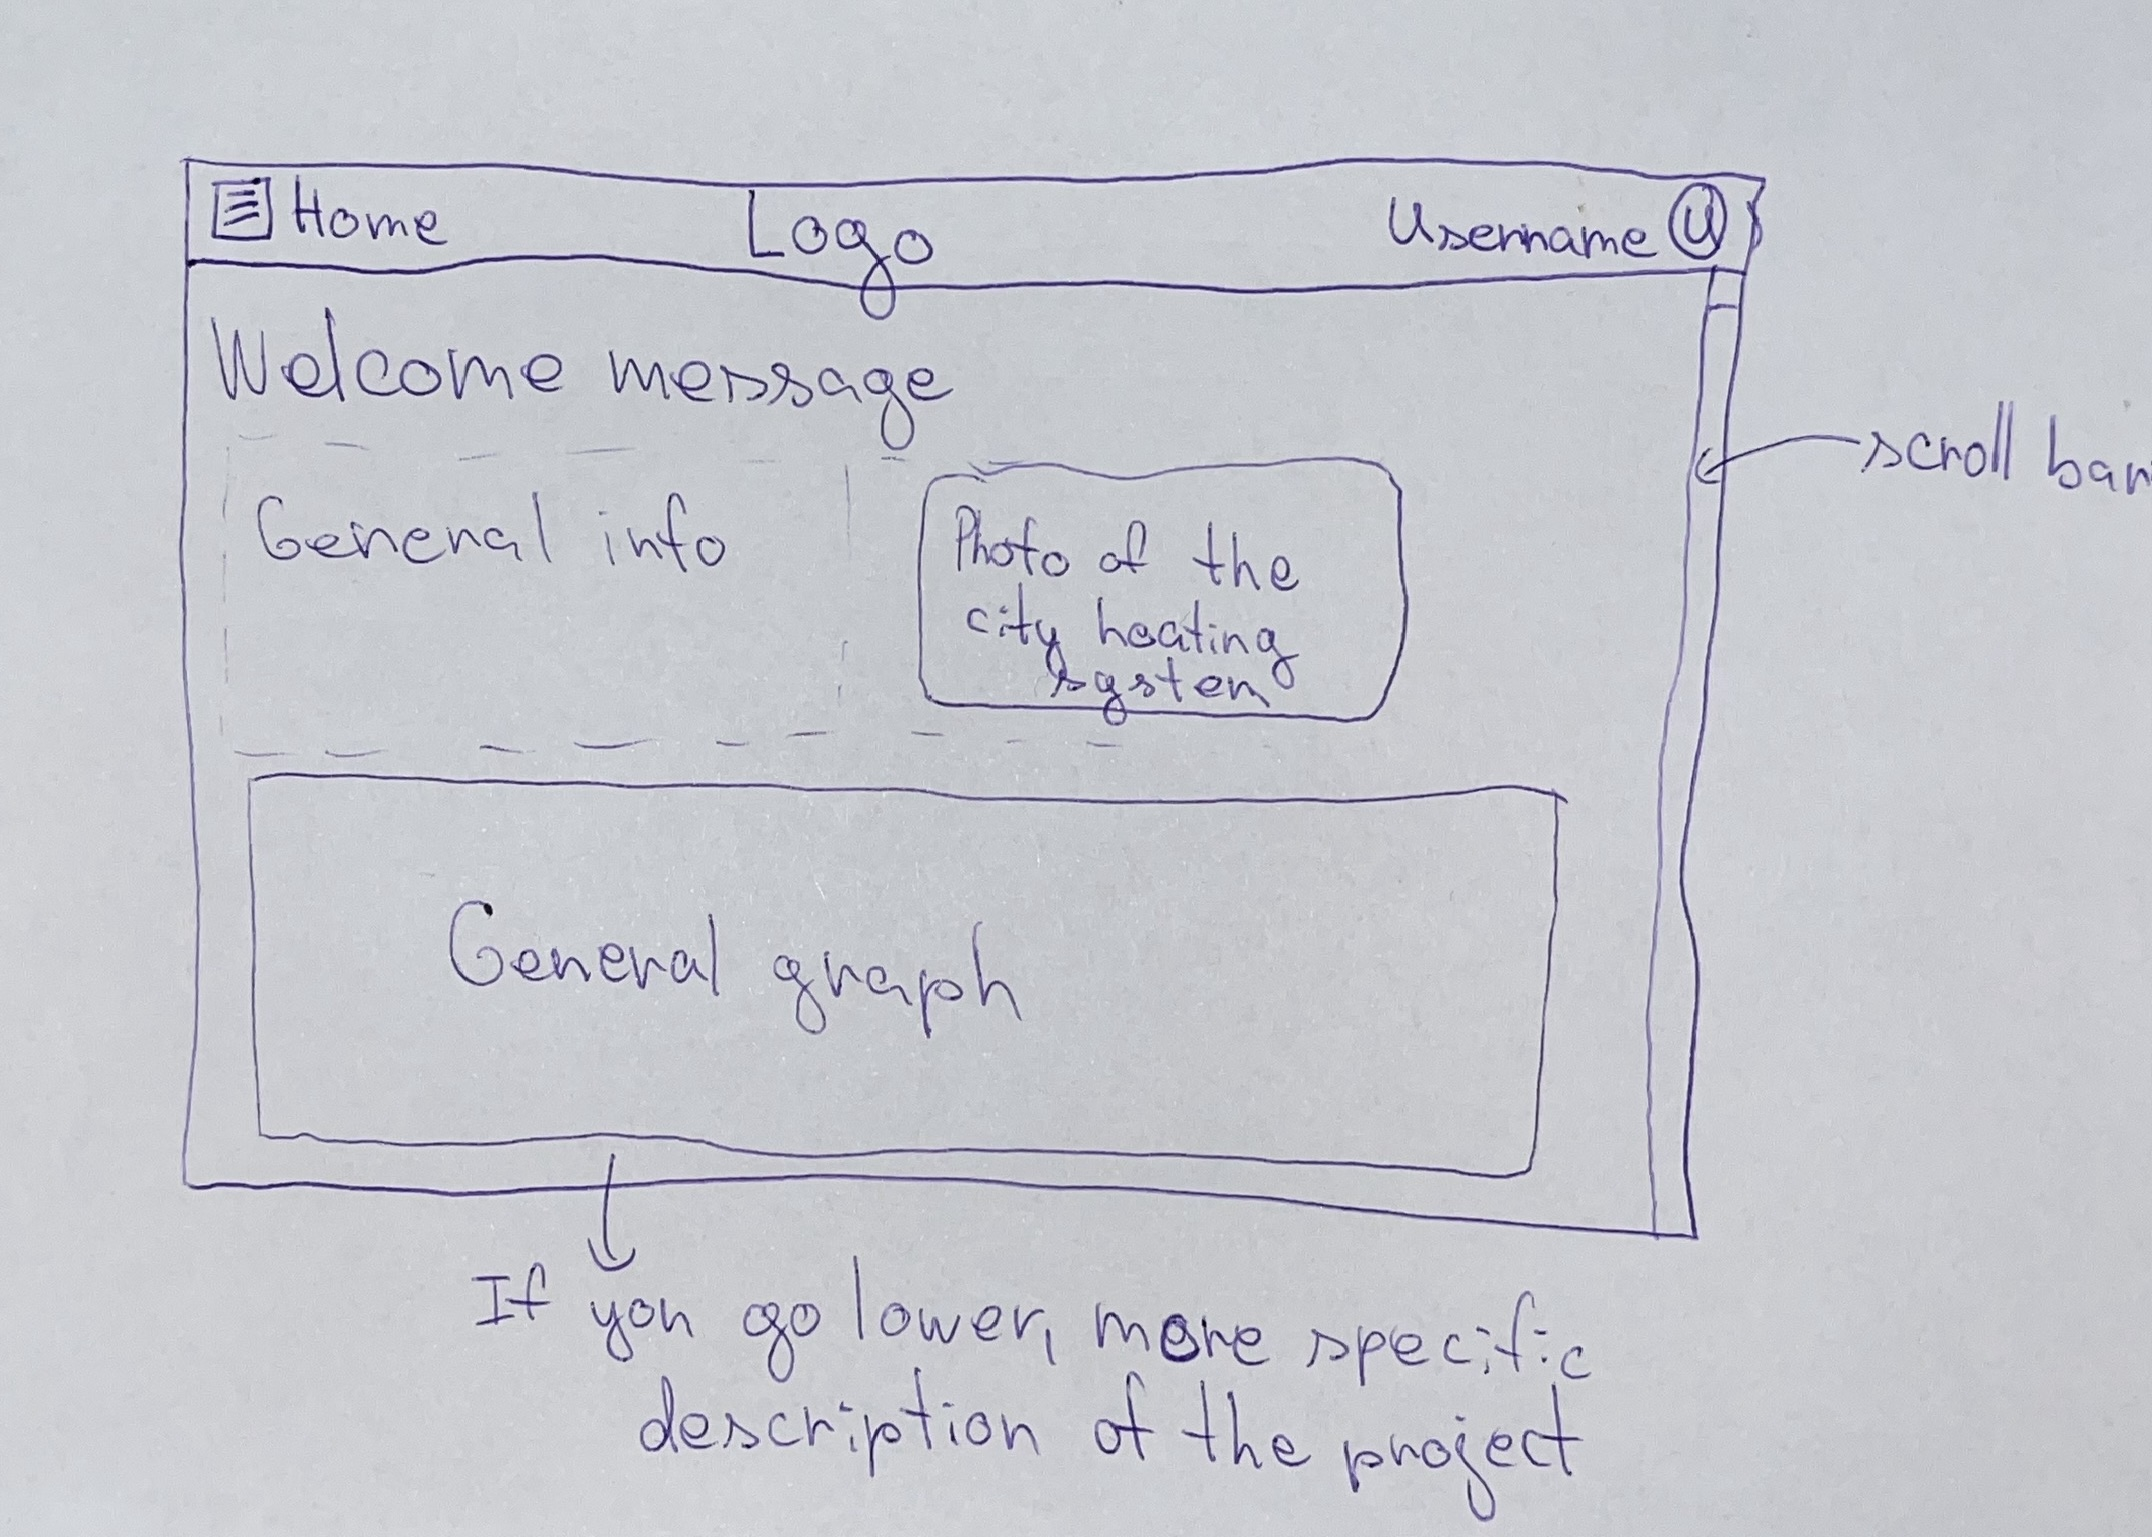
\includegraphics[width=1\textwidth]{ZojaSketch1.png}
    \label{fig:ZojaSketch1}
\end{figure}
\newpage

\begin{figure}[h]
    \centering
    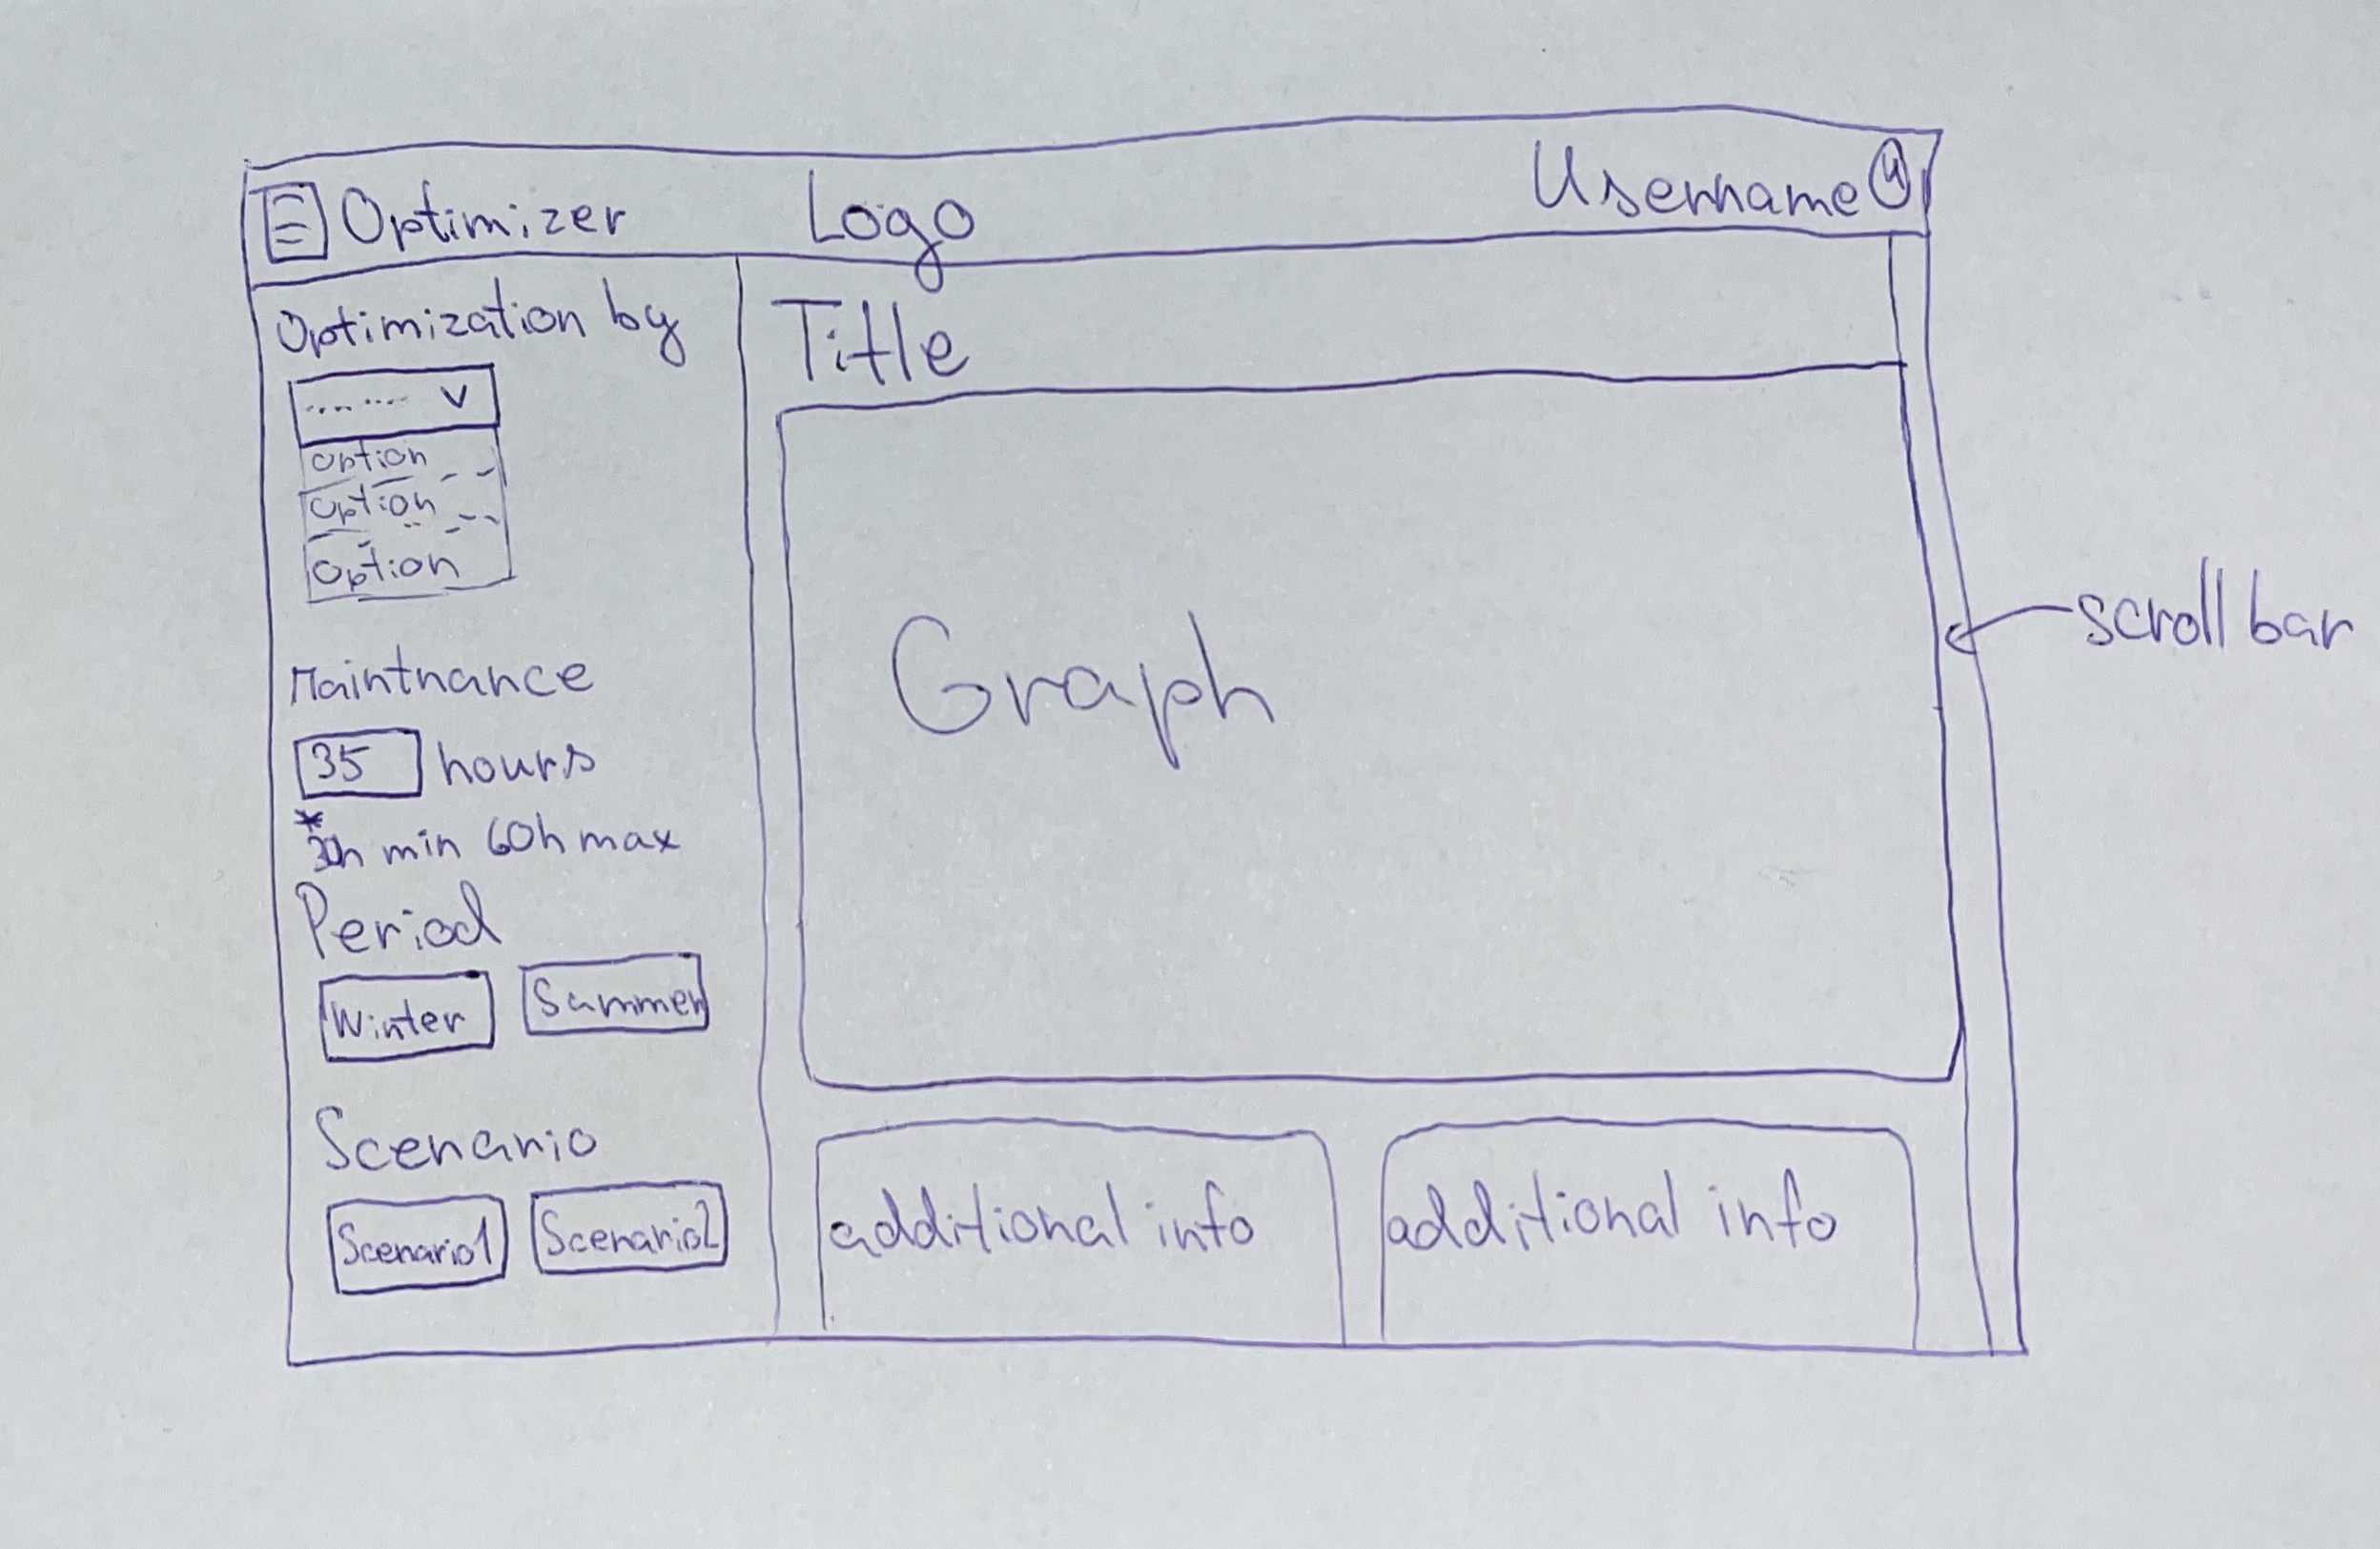
\includegraphics[width=1\textwidth]{ZojaSketch2.png}
    \label{fig:ZojaSketch2}
\end{figure}
\newpage

\begin{figure}[h]
    \centering
    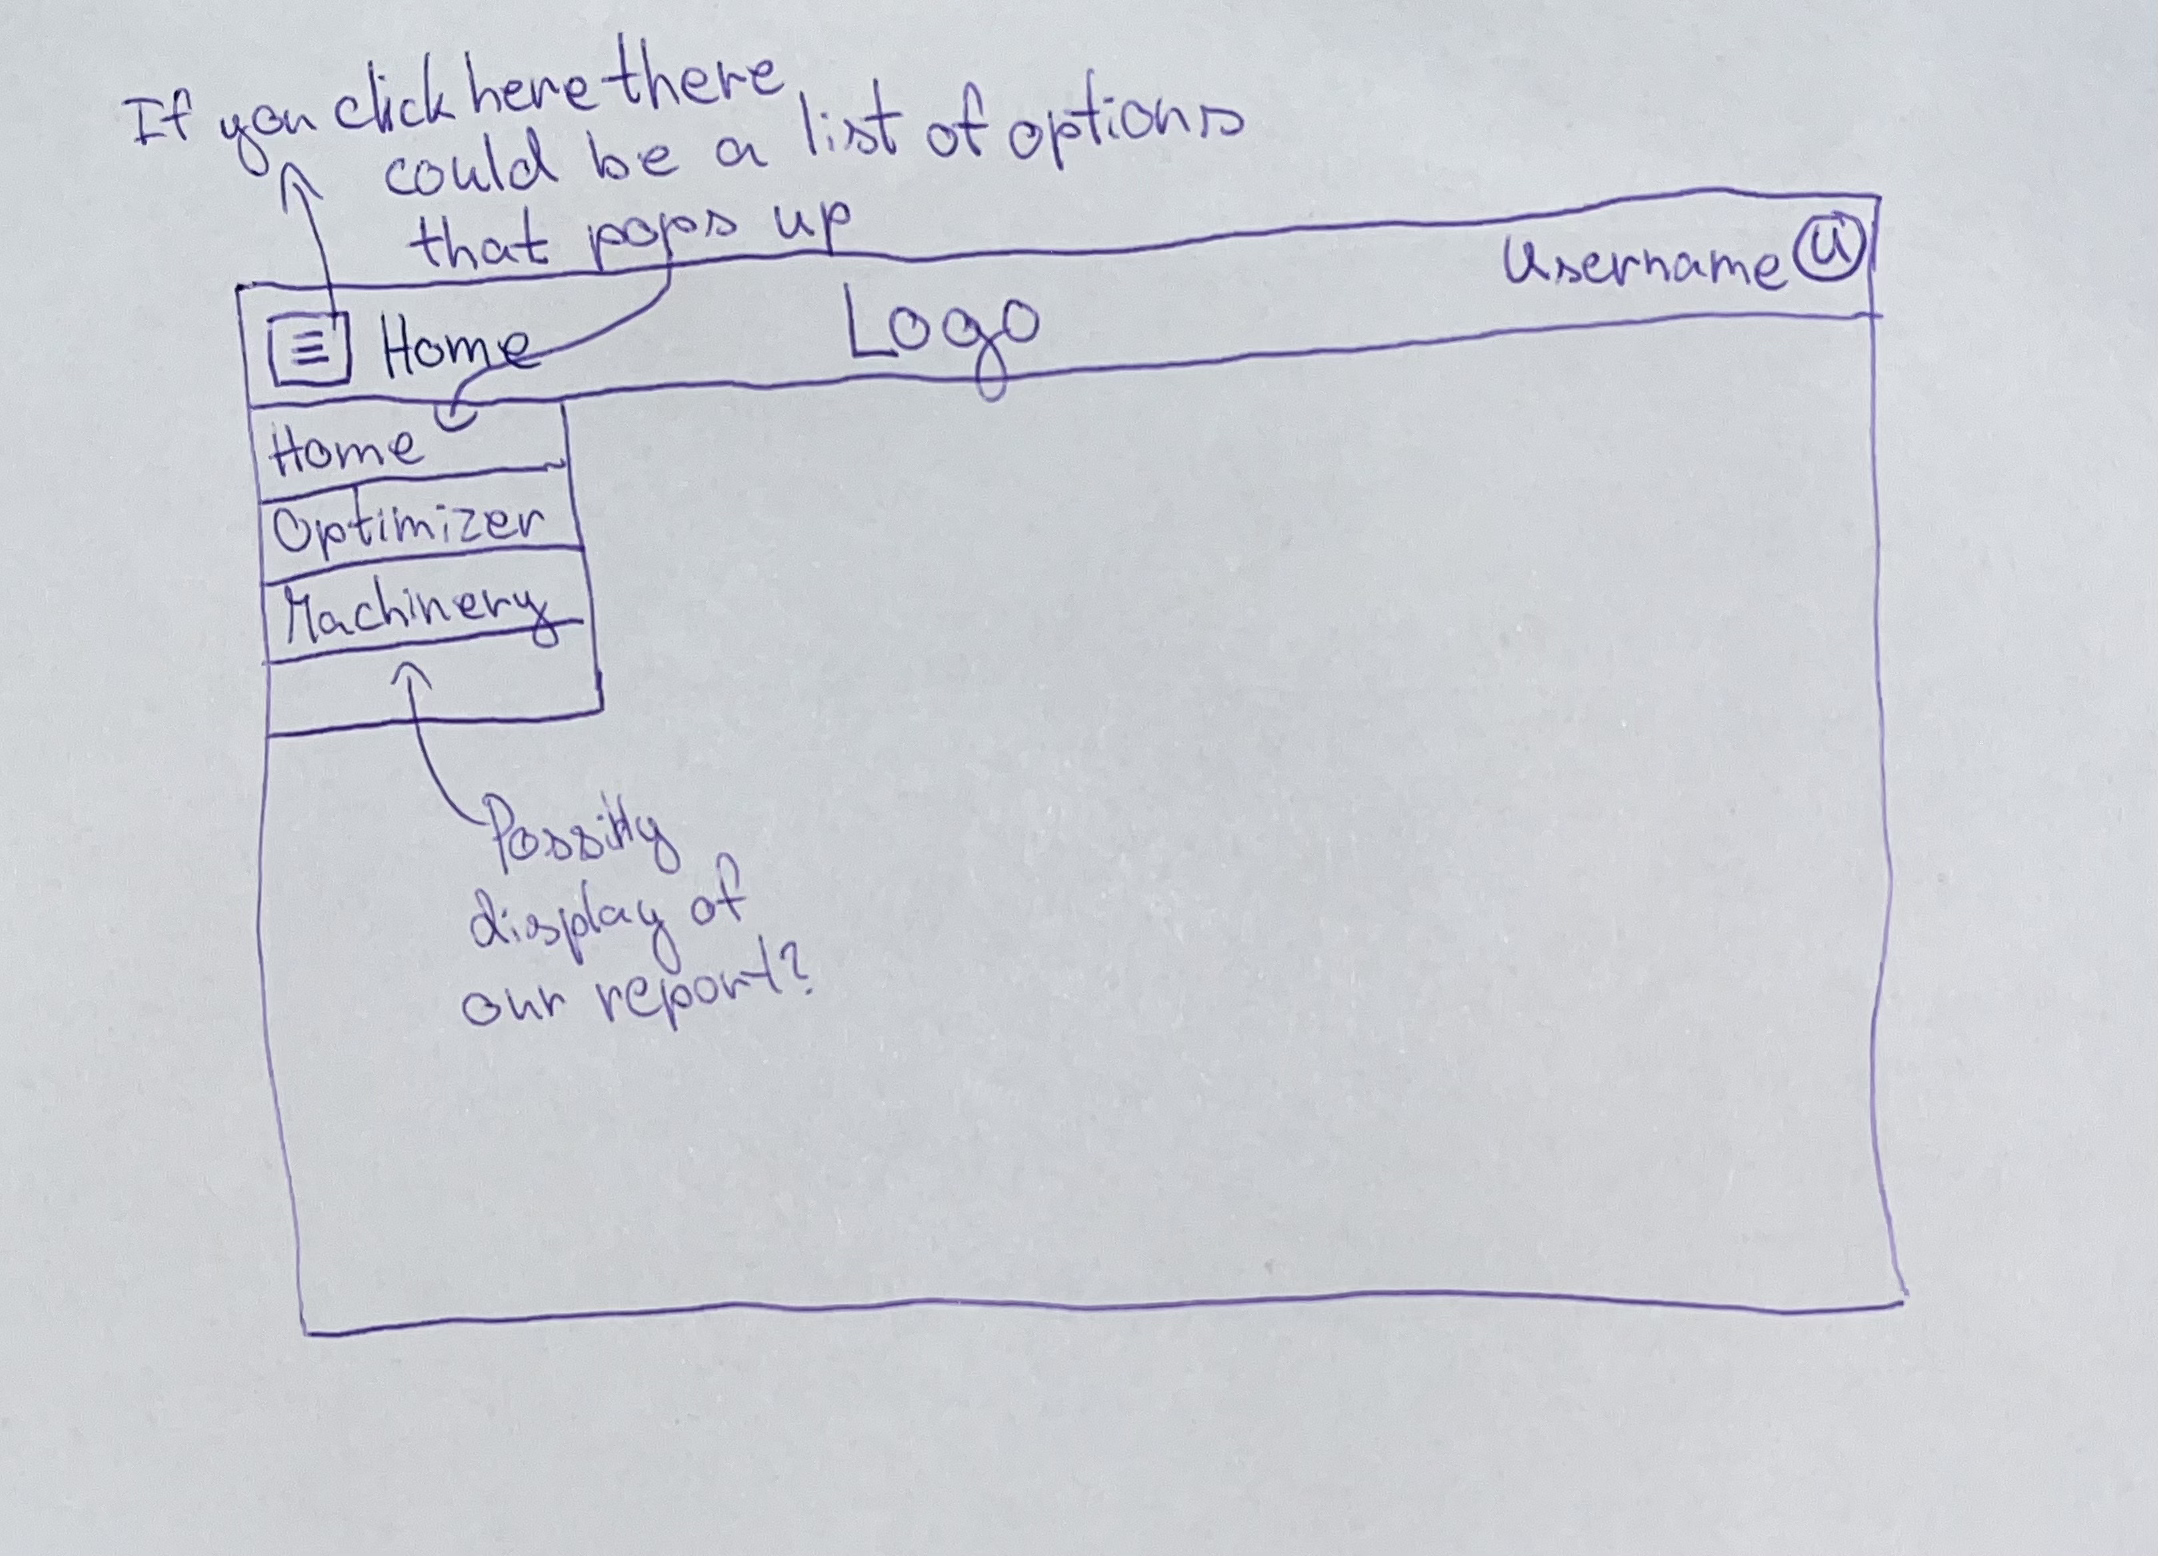
\includegraphics[width=1\textwidth]{ZojaSketch3.png}
    \label{fig:ZojaSketch3}
\end{figure}
\newpage

\begin{figure}[h]
    \centering
    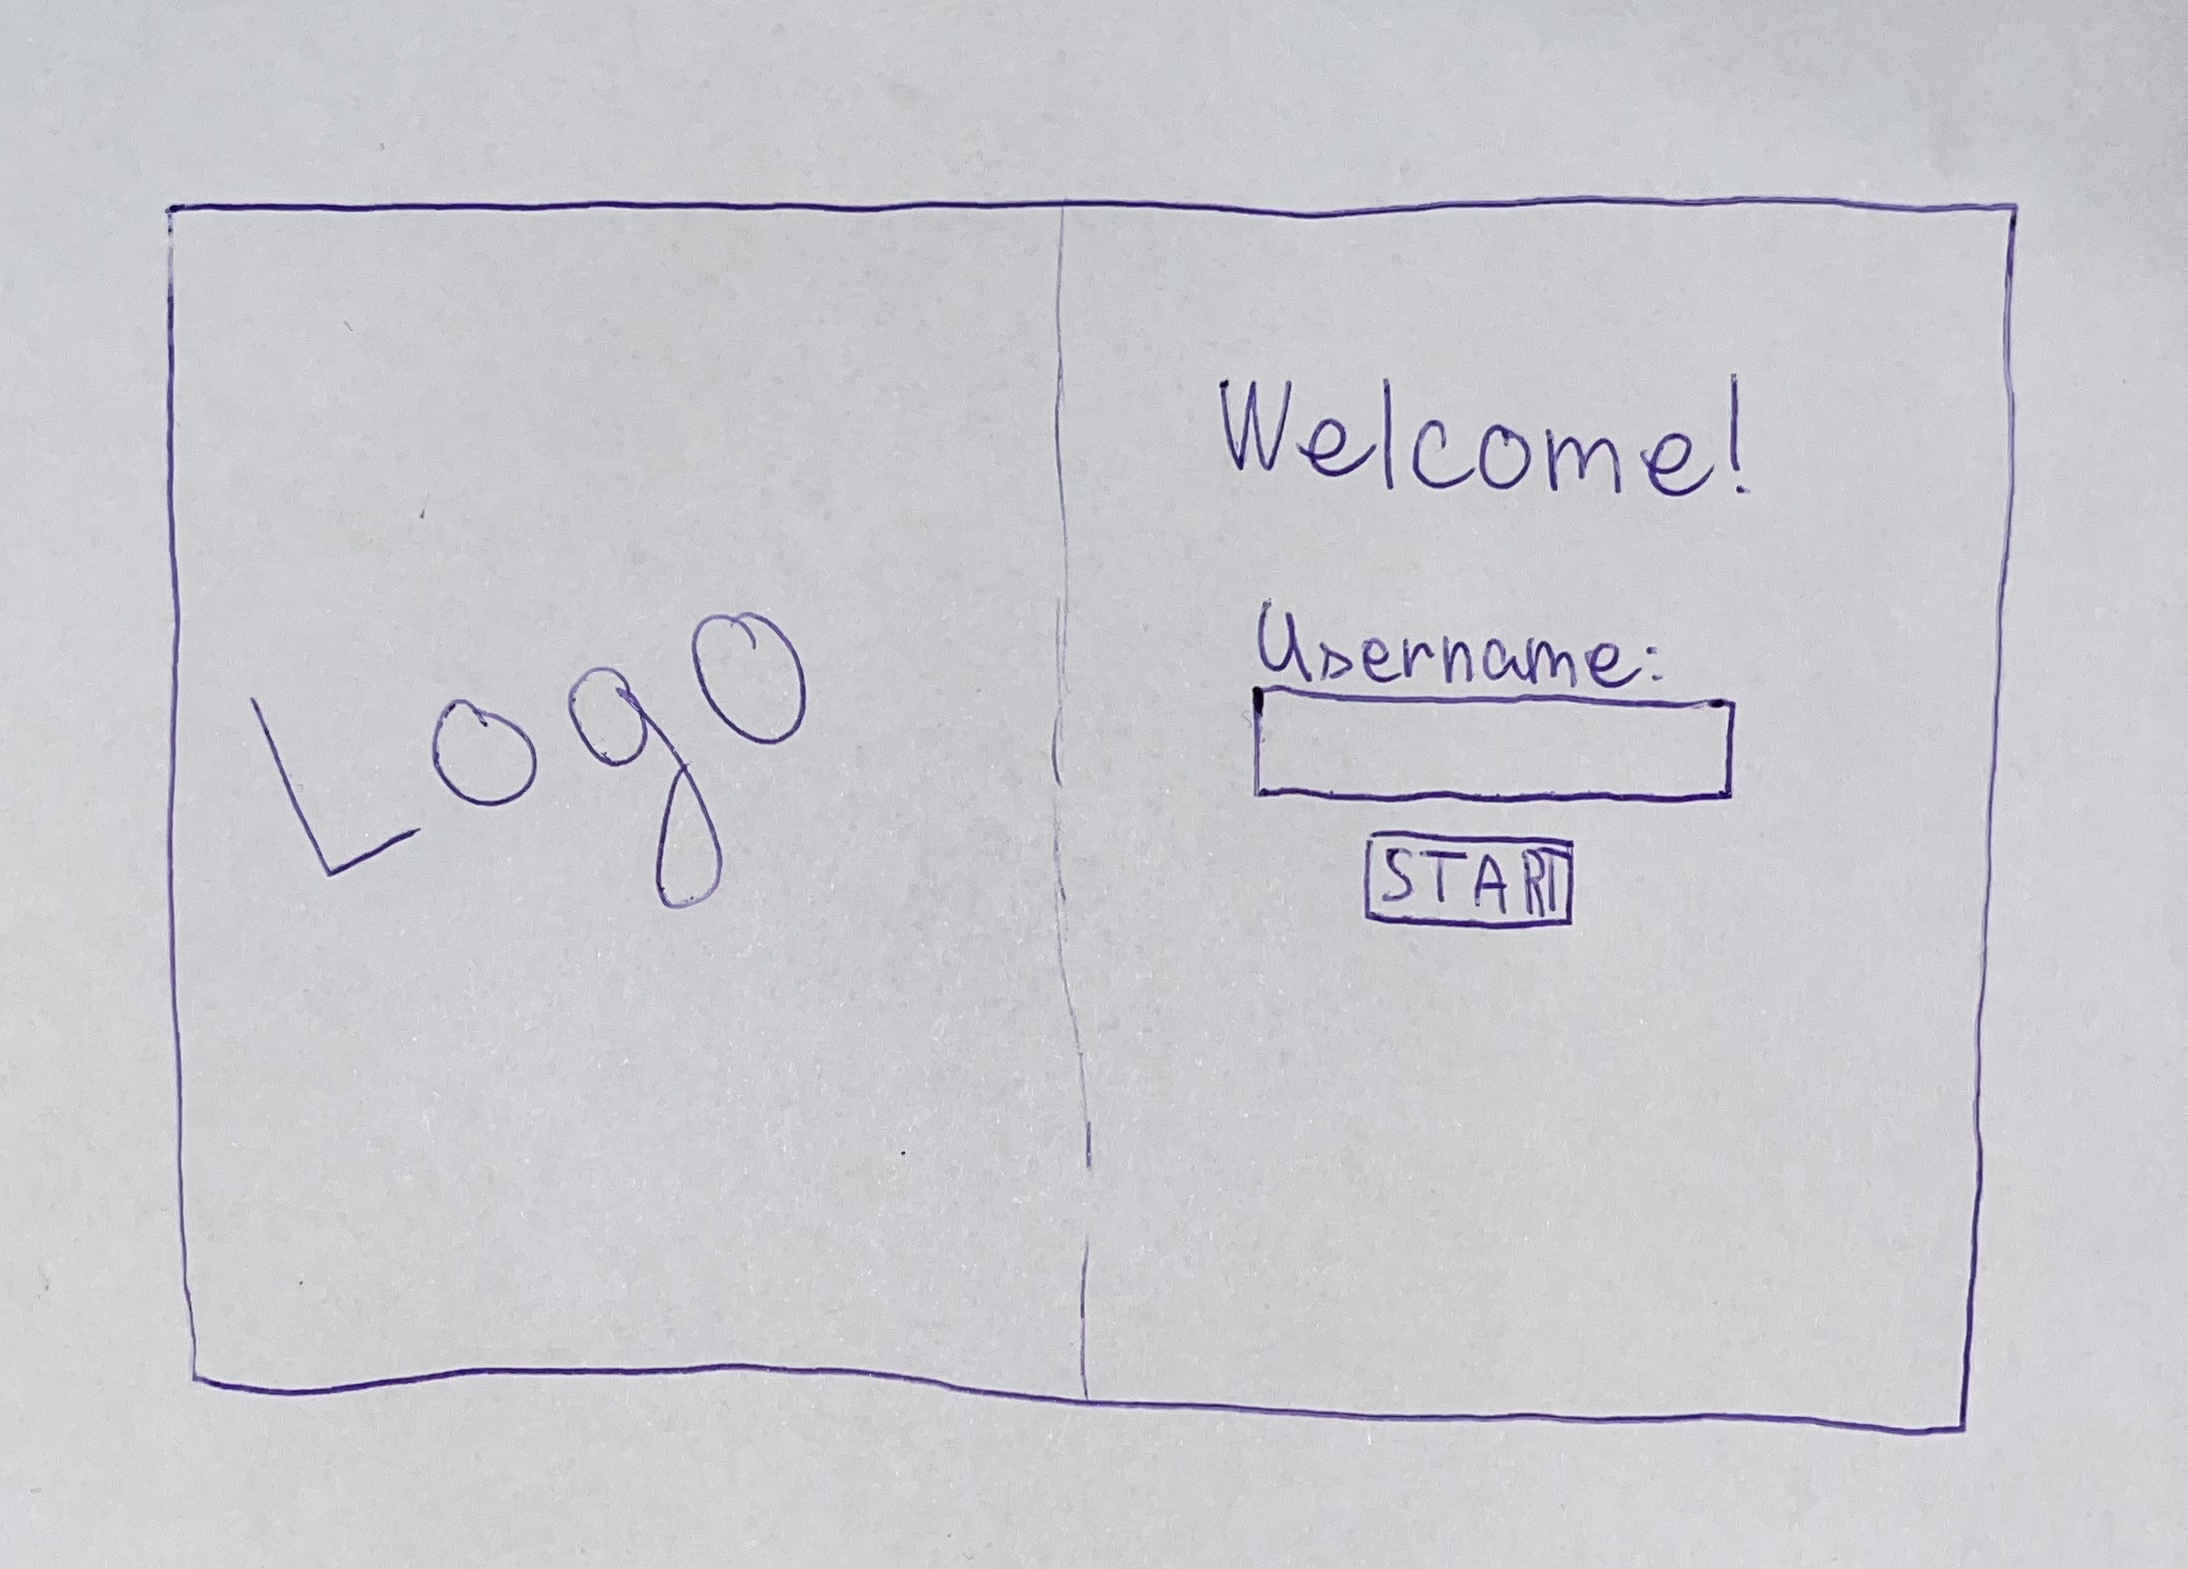
\includegraphics[width=1\textwidth]{ZojaSketch4.png}
    \label{fig:ZojaSketch4}
\end{figure}
\newpage

\begin{figure}[h]
    \centering
    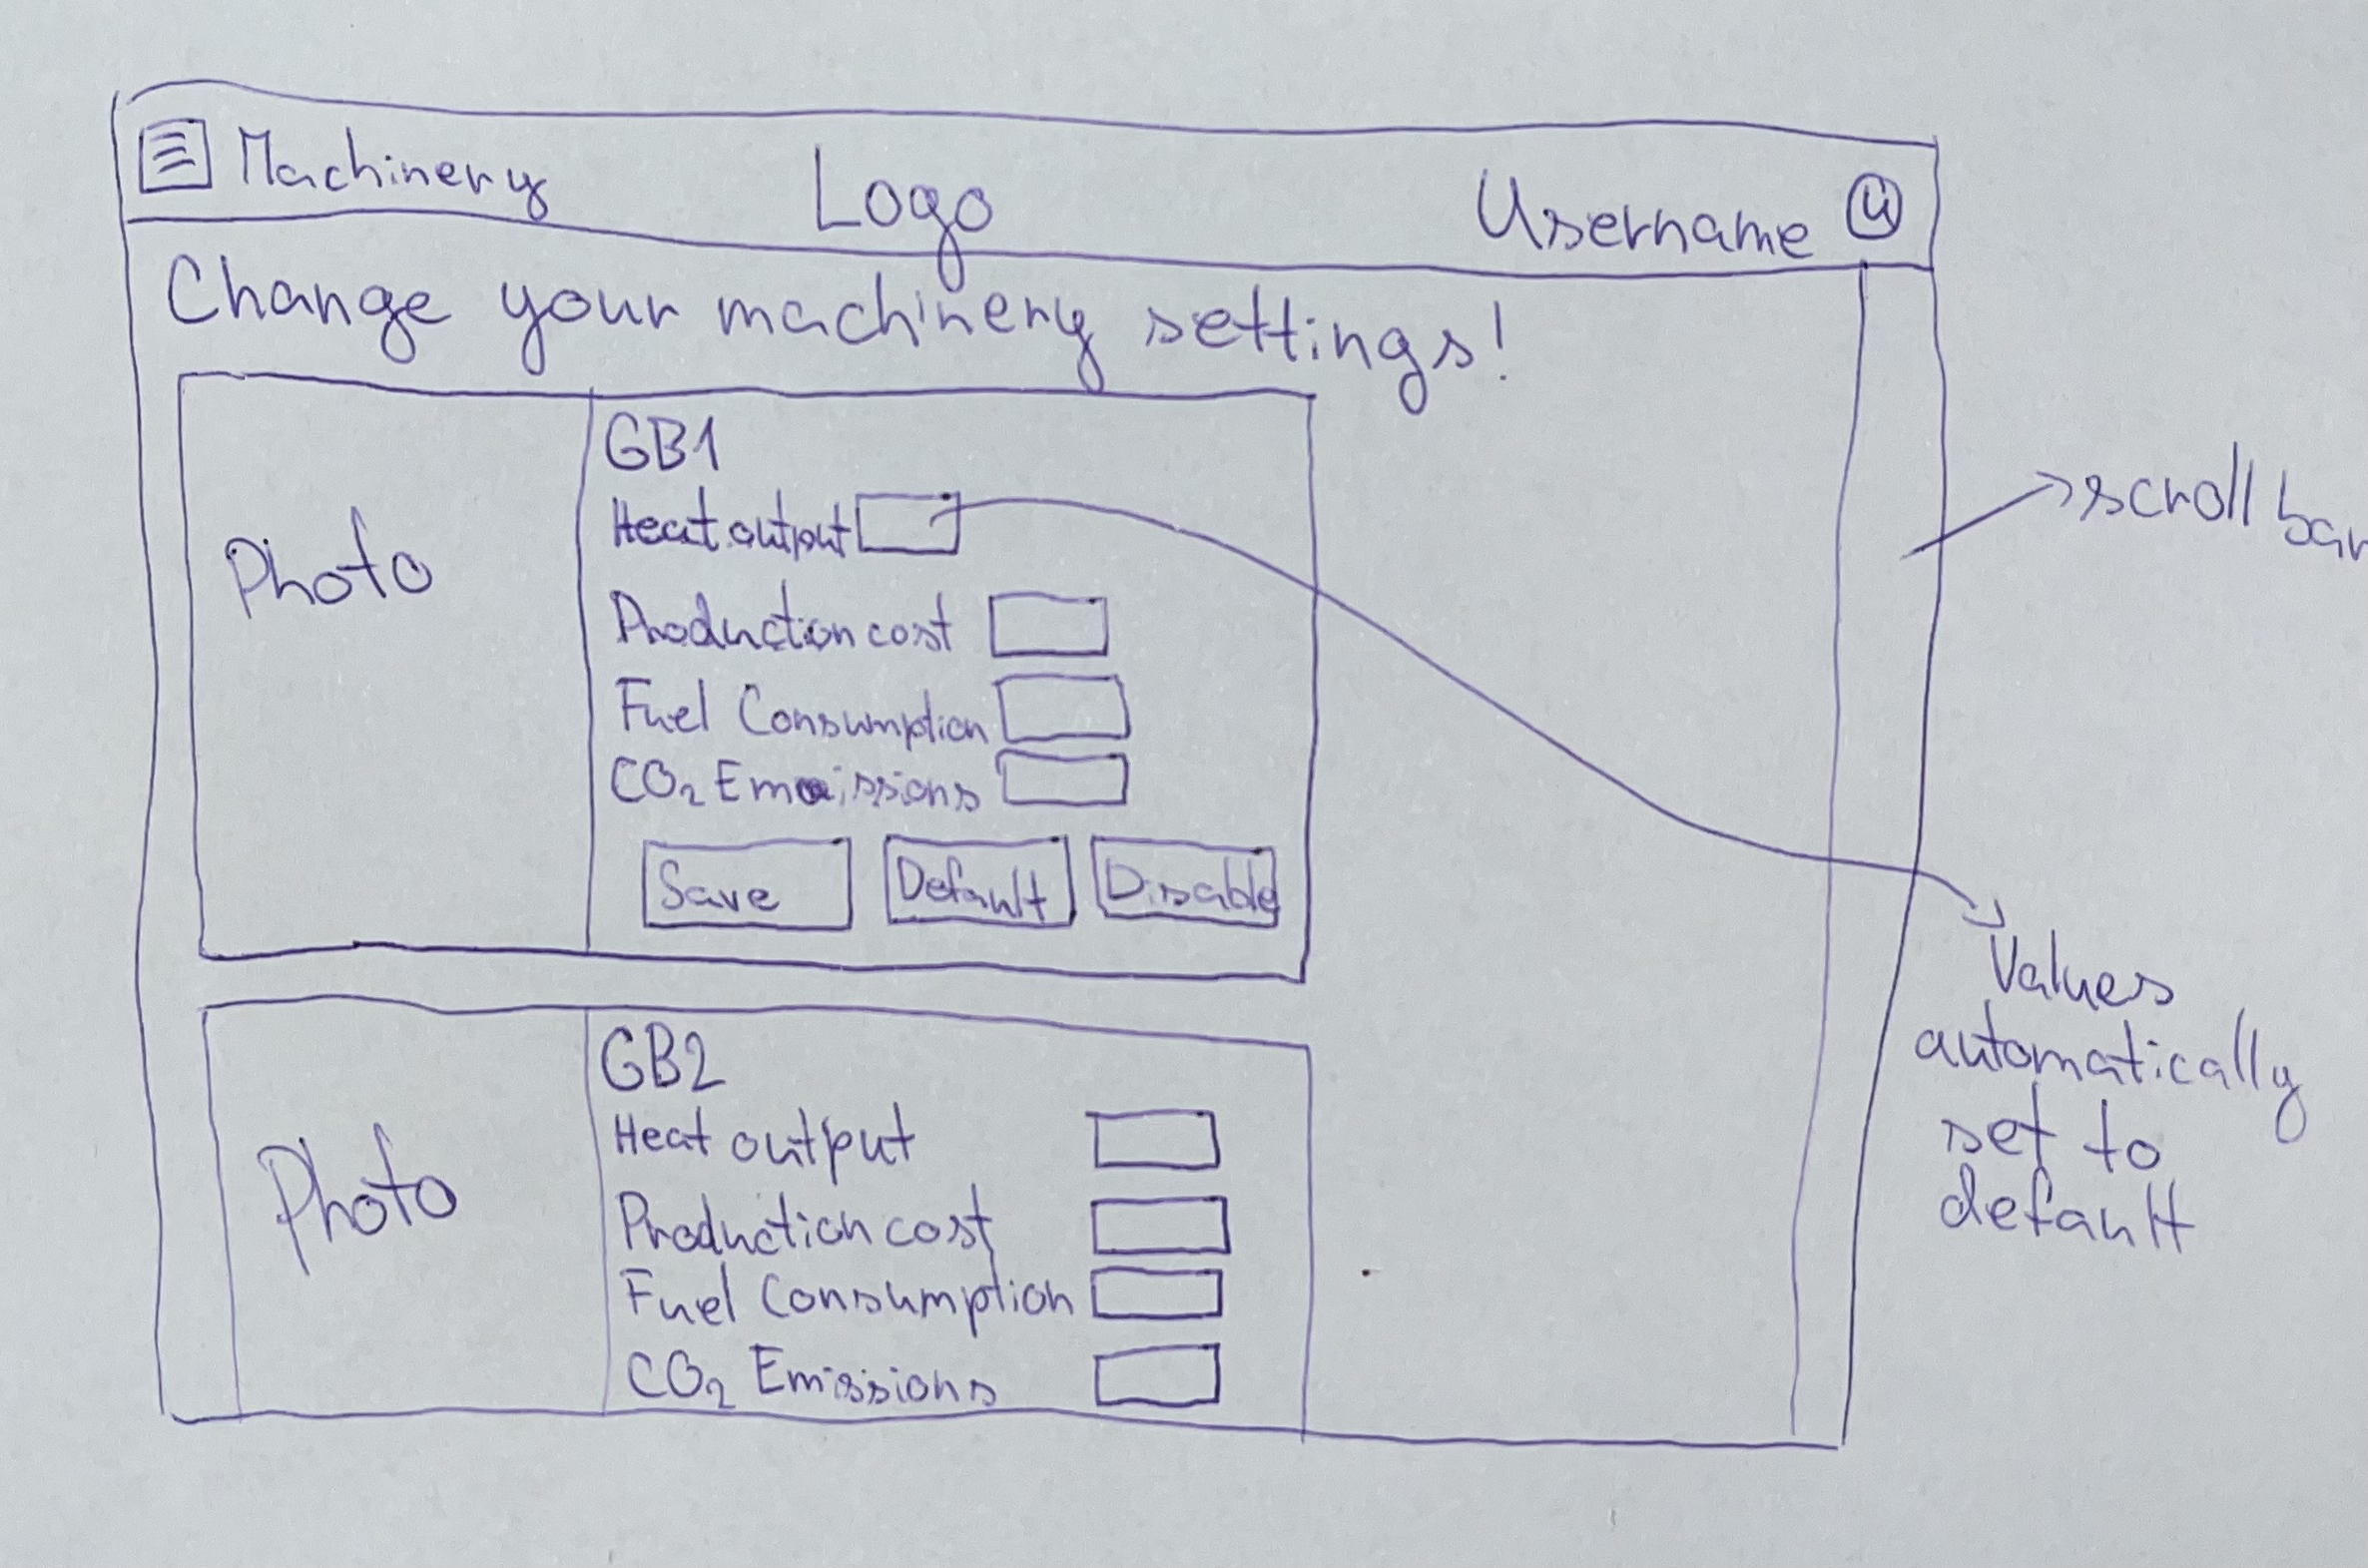
\includegraphics[width=1\textwidth]{ZojaSketch5.png}
    \label{fig:ZojaSketch5}
\end{figure}
\newpage

Zoe's Sketch:
\begin{figure}[h]
    \centering
    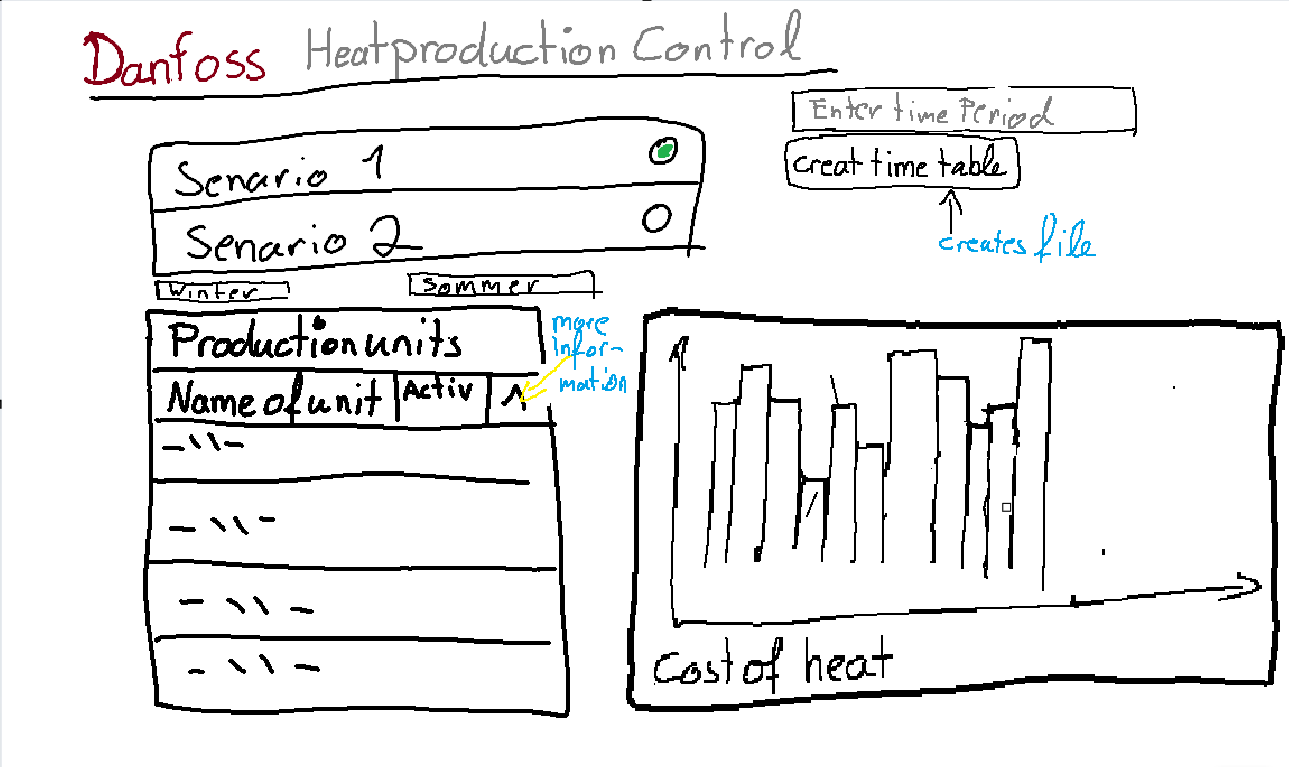
\includegraphics[width=1\textwidth]{ZoeSketch.png}
    \label{fig:ZoeSketch}
\end{figure}                                   % Call file with appendix

% -------------------------------------------------------------
% BIBLIOGRAPHY 
% -------------------------------------------------------------
\addcontentsline{toc}{chapter}{References}
\bibliographystyle{IEEEtran}
\bibliography{References}


% -------------------------------------------------------------
% END DOCUMENT CONTENT
% -------------------------------------------------------------
\end{document}




